% ========== Template by IC\M/T Institute of Creative\Media/Technologies =============
% ==========  M. Wagner and K. Blumenstein, 2021 ============= 
% ==========  Based on the LaTeX Thesis Template for the University of Applied Sciences St.Pölten by P. Lechner https://github.com/hrtlacek/ThesisTemplate-FH-StP        ============= 

%----------------------------------------------------------------
% TODO List


%----------------------------------------------------------------

% ============= Settings for the Work =============

%***************************************************************************************

% Place your data here!!!

\def\workTitle{Field Theories \& \\ Canonical Quantization}
\def\subTitle{~}
\def\specialization{<Name of Masterclass>}
\def\studentFirstName{Mukund V, Pugazharasu A D, and Rishi Kumar}
%\def\studentLastName{A D}
\def\studentId{18-UPH-311, 18-UPH-313, 18-UPH-347}
\def\advisorPreTitle{Prof.}
\def\advisoFirstName{T. R.}
\def\advisorLastName{Govindarajan}
\def\advisorPosTitle{Adjunct Factuly, IMSc, Chennai}
\def\assessorPreTitle{Dr.}
\def\assessorFirstName{A. Stanley}
\def\assessorLastName{Raj}
\def\assessorPosTitle{Assistant Professor, Loyola Colelge, Chennai}
\def\place{Loyola College, Chennai}
\def\dateDay{25}
\def\dateMonth{04}
\def\dateYear{2021}

%***************************************************************************************

\newif\ifUseOneSide                         % <== DONT TOUCH THIS!!!
\newif\ifUseGermanVersion				    % <== DONT TOUCH THIS!!!
\newif\ifUseMasterInteractiveTechnologies 	% <== CAN'T TOUCH THIS!!! (da da dada)
\newif\ifUseMasterDigitalDesign	            % <== DONT TOUCH THIS!!!
\newif\ifUseMasterDigitalMediaProduction	% <== DONT TOUCH THIS!!!
\newif\ifUseMasterDigitalHealthCare			% <== DONT TOUCH THIS!!!
\newif\ifUseBachelorMediaTechnologiesOne    % <== DONT TOUCH THIS!!!
\newif\ifUseBachelorMediaTechnologiesTwo    % <== DONT TOUCH THIS!!!
\newif\ifUseBachelorSmartEngineeringOne     % <== DONT TOUCH THIS!!!
\newif\ifUseBachelorSmartEngineeringTwo     % <== DONT TOUCH THIS!!!
\newif\ifUseBachelorCreativeComputingOne    % <== DONT TOUCH THIS!!!
\newif\ifUseBachelorCreativeComputingTwo    % <== DONT TOUCH THIS!!!

%To switch between one or two side layout
\UseOneSidetrue                             % Using the one side layout
%\UseOneSidefalse                            % Using the two side layout
% *** ATTENTION: When using double page layout, you need to print the Title Page as a single Page!!! ***

%***************************************************************************************

% To switch the version please use the comment "%" option :-). After a language change, you have to rebuild the whole project (in Overleaf --> recompile from scratch) 
%\UseGermanVersiontrue					    % German version
\UseGermanVersionfalse					    % English version

%***************************************************************************************

% To switch between the study programs use the comment option :-) 
% !!!ATTENTION: Only one has to be activated!!!
%\UseBachelorMediaTechnologiesOnetrue		% Bachelor #1 Media Technology
%\UseBachelorMediaTechnologiesTwotrue		% Bachelor #2 Media Technology
%\UseBachelorSmartEngineeringOnetrue		% Bachelor #1 Smart Engineering
%\UseBachelorSmartEngineeringTwotrue		% Bachelor #2 Smart Engineering
%\UseBachelorCreativeComputingOnetrue		% Bachelor #1 Creative Computing
%\UseBachelorCreativeComputingTwotrue		% Bachelor #2 Creative Computing
\UseMasterInteractiveTechnologiestrue		% Master Interactive Technologies
%\UseMasterDigitalDesigntrue		        % Master Digital Design
%\UseMasterDigitalMediaProductiontrue		% Master Digital Media Production
%\UseMasterDigitalHealthCaretrue			% Master Digital Health Care

%***************************************************************************************

%Dokumentklasse without end dot ;-)
%\documentclass[a4paper,twoside,11pt, numbers=noenddot]{scrreprt}
\ifUseOneSide
    \documentclass[a4paper,oneside,11pt, numbers=noenddot]{scrreprt}%{book}{report}
\else
    \documentclass[a4paper,twoside,11pt, numbers=noenddot]{scrreprt}%{book}{report}
\fi

\usepackage[left= 3.5cm,right = 3cm, bottom = 3.5 cm, top = 3 cm]{geometry}
\usepackage[onehalfspacing]{setspace}
\usepackage{physics}
\usepackage{biblatex}
\addbibresource{Bibliography.bib}
\usepackage{tcolorbox}
\tcbuselibrary{skins}
\usepackage{lipsum}
\usepackage{amsmath}
% Standard Packages
\usepackage[utf8]{inputenc}

% ============= Packages =============

% Document information
\usepackage[
	pdftitle={\workTitle},
	pdfsubject={},
	pdfauthor={\studentFirstName \studentLastName},
	pdfkeywords={}
	pdftex=true, 
	colorlinks=true,
 	breaklinks=true,
	citecolor=black,
	linkcolor=black,	
	menucolor=black,	
	urlcolor=black
]{hyperref}

\hypersetup{
    %bookmarks=true,         % show bookmarks bar?
    unicode=false,          % non-Latin characters in Acrobat’s bookmarks
    pdftoolbar=true,        % show Acrobat’s toolbar?
    pdfmenubar=true,        % show Acrobat’s menu?
    pdffitwindow=false,     % window fit to page when opened
    pdfstartview={FitH},    % fits the width of the page to the window
    pdftitle={My title},    % title
    pdfauthor={Author},     % author
    pdfsubject={Subject},   % subject of the document
    pdfcreator={Creator},   % creator of the document
    pdfproducer={Producer}, % producer of the document
    pdfkeywords={keyword1} {key2} {key3}, % list of keywords
    pdfnewwindow=true,      % links in new window
    colorlinks=false,       % false: boxed links; true: colored links
    linkcolor=black,          % color of internal links (change box color with linkbordercolor)
    citecolor=black,        % color of links to bibliography
    filecolor=black,      % color of file links
    urlcolor=black           % color of external links
}

\usepackage{csquotes}

\usepackage[T1]{fontenc}
\usepackage{graphicx, subfigure}
\usepackage{fancyhdr}
\usepackage{lmodern}
\usepackage{color}
\usepackage{transparent}

\usepackage[backend=biber, style=apa, citestyle=authoryear, sorting=nyt]{biblatex}

% Switch the language
\ifUseGermanVersion
    \DeclareLanguageMapping{ngerman}{ngerman-apa}
\else
    \DeclareLanguageMapping{english}{english-apa}
\fi

\addbibresource{biblatex.bib}

% Additional letters from the American Mathematical Society
\usepackage{amsfonts}
\usepackage{mathtools}

\usepackage[export]{adjustbox}

% Block Diagram Drawing Package
% ---tikz
\usepackage{tikz}
\usetikzlibrary{positioning}
\usepackage{pgfplots}
\pgfplotsset{compat=1.10}
\usepackage{textcomp}

%Package for using the [H] option on graphics to force them into place
\usepackage{float}

%iPython packages:
%\usepackage{graphicx} % Used to insert images
\usepackage{adjustbox} % Used to constrain images to a maximum size 
\usepackage{color} % Allow colors to be defined
\usepackage{enumerate} % Needed for markdown enumerations to work
\usepackage{geometry} % Used to adjust the document margins
\usepackage{amsmath} % Equations
\usepackage{amssymb} % Equations
%\usepackage[mathletters]{ucs} % Extended unicode (utf-8) support
% \usepackage[utf8x]{inputenc} % Allow utf-8 characters in the tex document
\usepackage{fancyvrb} % verbatim replacement that allows latex
\usepackage{grffile} % extends the file name processing of package graphics 
                         % to support a larger range 
    % The hyperref package gives us a pdf with properly built
    % internal navigation ('pdf bookmarks' for the table of contents,
    % internal cross-reference links, web links for URLs, etc.)
\usepackage{hyperref}
\usepackage{longtable} % longtable support required by pandoc >1.10
\usepackage{tabularx}
\usepackage{epigraph}
\usepackage{quotchap}
\usepackage{lscape}
\usepackage{enumerate}
% embedding of audio/video files etc.
% \usepackage{attachfile}
% \usepackage{movie15}
% \usepackage{media9}
% \usepackage{menukeys}

\usepackage[labelfont=it, labelsep=period, format=plain,justification=raggedright, singlelinecheck=false]{caption}
\captionsetup[figure]{justification=centering}
\definecolor{light-gray}{gray}{0.85}

% Switch between German and English based on the Settingx.tex. file
\usepackage{ifthen}

% =============== Block Diagram Drawing Config
\usetikzlibrary{shapes,arrows}

% Definition of blocks:
\tikzset{%
  block/.style    = {draw, thick, rectangle, minimum height = 3em,
    minimum width = 3em},
  sum/.style      = {draw, circle, node distance = 2cm}, % Adder
  input/.style    = {coordinate}, % Input
  output/.style   = {coordinate}, % Output
  mult/.style	  = {draw, isosceles triangle, minimum height=1cm, minimum width =1cm}
}
%mult/.style	  = {isosceles triangle, sharp corners, anchor=center, xshift=-4mm, minimum height=1.5cm, minimum width =0.05cm}
%isosceles triangle, fill=gray!25, minimum width=1.5cm

% Defining string as labels of certain blocks.
\newcommand{\suma}{\Large$+$}
\newcommand{\inte}{$\displaystyle \int$}
\newcommand{\derv}{\huge$\frac{d}{dt}$}
\newcommand{\conv}{\huge$\ast$}

\DeclareMathAlphabet{\mathcalligra}{T1}{calligra}{m}{n}
\DeclareFontShape{T1}{calligra}{m}{n}{<->s*[2.2]callig15}{}
\newcommand{\scriptr}{\mathcalligra{r}\,}
\newcommand{\boldscriptr}{\pmb{\mathcalligra{r}}\,}
% ============================================

% -- Settings für Code abbildungen
\usepackage{listings,lstautogobble}
\lstset{backgroundcolor=\color{light-gray},frame=single, framerule=0pt, showspaces=false, showtabs=false, numbers=left, numbersep=5pt, breaklines=false, autogobble=true, language=C++}

% Setze arial font
\usepackage[scaled]{helvet}
\renewcommand*{\familydefault}{\sfdefault}

% FH-green blue
\definecolor{FH}{rgb}{0.10, 0.57, 0.68}
% FH-green blue 2
\definecolor{FH2}{rgb}{0.0392, 0.666, 0.549}

% No indention afer a paragraph
\setlength{\parindent}{0cm}

% Paragraph
\setlength{\parskip}{0.3cm}

% ============= Header and Footer =============

\renewcommand{\chaptermark}[1]{\markboth{\thechapter~ #1}{}}

\ifUseOneSide
\fancypagestyle{icmt}{%
  \fancyhf{}% Clear header and footer
  \fancyhead[L]{\leftmark}
  \fancyfoot[R]{\thepage}% Custom footer
  \renewcommand{\headrulewidth}{0.4pt}% Line at the header visible
  \renewcommand{\footrulewidth}{0.0pt}% Line at the footer visible
}
% Redefine the plain page style
\fancypagestyle{plain}{%
  \fancyhf{}%
  \fancyfoot[R]{\thepage}%
  \renewcommand{\headrulewidth}{0.0pt}% Line at the header invisible
  \renewcommand{\footrulewidth}{0.0pt}% Line at the footer visible
}
\else
\fancypagestyle{icmt}{%
  \fancyhf{}% Clear header and footer
  \fancyhead[L]{\leftmark}
  \fancyfoot[RO,LE]{\thepage}% Custom footer
  \renewcommand{\headrulewidth}{0.4pt}% Line at the header visible
  \renewcommand{\footrulewidth}{0.0pt}% Line at the footer visible
}
% Redefine the plain page style
\fancypagestyle{plain}{%
  \fancyhf{}%
  \fancyfoot[RO,LE]{\thepage}%
  \renewcommand{\headrulewidth}{0.0pt}% Line at the header invisible
  \renewcommand{\footrulewidth}{0.0pt}% Line at the footer visible
  }
\fi

% ============= Package Settings & Others ============= 


% Special Spellings
\hyphenation{De-zi-mal-tren-nung St-rei-fen-licht-scan-nern}

% Roman itemization \RM{<Number>}
\newcommand{\RM}[1]{\MakeUppercase{\romannumeral #1}}


% ============= Dokumentbeginn =============

\begin{document}

% Select the right main page ;-)
\ifUseGermanVersion
	
% setup page dimensions for titlepage
\newgeometry{left=2.4cm,right=2.4cm,bottom=2.5cm,top=2cm}

% force baselineskip and parindent
%\newlength{\tmpbaselineskip}
%\setlength{\tmpbaselineskip}{\baselineskip}
%\setlength{\baselineskip}{13.6pt}
%\newlength{\tmpparindent}
%\setlength{\tmpparindent}{\parindent}
%\setlength{\parindent}{17pt}

% first titlepage
\pagestyle{empty}

\begin{figure}[H]
\vspace*{-2.5cm}
\hspace*{2.5cm}

\includegraphics[keepaspectratio, width=1.4\textwidth, right]{TemplateElements/fhLogo3.png}
\end{figure}



\begin{center}

\vspace{1cm}

\begin{minipage}[t][5cm][s]{\textwidth}%
\centering
\Huge{{\color{FH2}{\fontsize{24}{30} \selectfont \workTitle\\}}}
\vspace{0.5cm}
\LARGE{{\color{FH2}{\fontsize{16}{24} \selectfont \subTitle\\}}}
\end{minipage}

\vspace{1cm}


\ifnum\ifUseBachelorMediaTechnologiesOne 1
\else\ifUseBachelorSmartEngineeringOne 1
\else\ifUseBachelorCreativeComputingOne 1
\else0
\fi\fi\fi
=1 
   	\LARGE{Research Paper}
\else
	\ifnum\ifUseBachelorMediaTechnologiesTwo 2
	\else\ifUseBachelorSmartEngineeringTwo 2
	\else\ifUseBachelorCreativeComputingTwo 2
\else0
\fi\fi\fi
=2
	\LARGE{Bachelorarbeit}
\else
	\ifUseMasterInteractiveTechnologies
		\LARGE{Masterarbeit}
	\else
	\ifUseMasterDigitalDesign
		\LARGE{Masterarbeit}
	\else
    \ifUseMasterDigitalMediaProduction
		\LARGE{Masterarbeit}
	\else
	\ifUseMasterDigitalHealthCare
		\LARGE{Masterarbeit}
    \else
        \LARGE{YOU HAVE TO CHOOSE THE PROGRAM TYPE IN THE SETTINGS!!!}
    \fi\fi\fi\fi
\fi\fi


\vspace{1.3cm}
\ifUseBachelorMediaTechnologiesOne
	\fontsize{11pt}{15pt}\selectfont Bachelor-Studiengang Medientechnik\\
Fachhochschule St. Pölten\\  
\else
	\ifUseBachelorMediaTechnologiesTwo
		\fontsize{11pt}{15pt}\selectfont Bachelor-Studiengang Medientechnik\\
Fachhochschule St. Pölten\\  
\else
	\ifUseBachelorSmartEngineeringOne
    	\fontsize{11pt}{15pt}\selectfont Bachelor-Studiengang Smart Engineering\\
Fachhochschule St. Pölten\\ 
\else
    \ifUseBachelorCreativeComputingOne
    	\fontsize{11pt}{15pt}\selectfont Bachelor-Studiengang Creative Computing\\
Fachhochschule St. Pölten\\ 
\else
	\ifUseBachelorSmartEngineeringTwo
    	\fontsize{11pt}{15pt}\selectfont Bachelor-Studiengang Smart Engineering\\
Fachhochschule St. Pölten\\ 
\else
    \ifUseBachelorCreativeComputingTwo
    	\fontsize{11pt}{15pt}\selectfont Bachelor-Studiengang Creative Computing\\
Fachhochschule St. Pölten\\ 
\else
	\ifUseMasterInteractiveTechnologies
		\fontsize{11pt}{15pt}\selectfont Ausgeführt zum Zweck der Erlangung des akademischen Grades\\
		\textbf{Dipl.-Ing. für technisch-wissenschaftliche Berufe}
\else
	\ifUseMasterDigitalDesign
		\fontsize{11pt}{15pt}\selectfont Ausgeführt zum Zweck der Erlangung des akademischen Grades\\
		\textbf{Dipl.-Ing. für technisch-wissenschaftliche Berufe}	
\else
    \ifUseMasterDigitalMediaProduction
		\fontsize{11pt}{15pt}\selectfont Ausgeführt zum Zweck der Erlangung des akademischen Grades\\
		\textbf{Dipl.-Ing. für technisch-wissenschaftliche Berufe}	
\else
	\ifUseMasterDigitalHealthCare
    	\fontsize{11pt}{15pt}\selectfont Ausgeführt zum Zweck der Erlangung des akademischen Grades\\
		\textbf{Master of Science in Engineering (MSc)}
    \else
        \LARGE{YOU HAVE TO CHOOSE THE PROGRAM TYPE IN THE SETTINGS!!!}
\fi\fi\fi\fi\fi\fi\fi\fi\fi\fi

\vspace{4mm}

\ifUseMasterInteractiveTechnologies
	am Masterstudiengang Interactive Technologies an der\\ 
Fachhochschule St. Pölten, Masterklasse \specialization
\else
    \ifUseMasterDigitalDesign
	am Masterstudiengang Digital Design an der\\ 
Fachhochschule St. Pölten, Masterklasse \specialization
\else
    \ifUseMasterDigitalMediaProduction
	am Masterstudiengang Digital Media Production an der\\ 
Fachhochschule St. Pölten, Masterklasse \specialization
\else
	\ifUseMasterDigitalHealthCare
		am Masterstudiengang Digital Healthcare\\ 
an der Fachhochschule St. Pölten
    \else
        
  	\fi\fi\fi\fi

\vspace{1cm}
\ifUseBachelorMediaTechnologiesOne
	Submitted by:
    
\else
	Ausgeführt von:\\ 
\fi
\fontsize{15pt}{15pt}\selectfont
\textbf{\studentFirstName\ \studentLastName} \\
\fontsize{11pt}{15pt}\selectfont
\studentId

\vspace{1cm}
\ifUseBachelorMediaTechnologiesOne
	\begin{tabular}{lll}
    Betreuer/in: & & \advisorPreTitle\ \advisoFirstName\ 		\advisorLastName, \advisorPosTitle\\
    %Zweitbegutachter/in: & & [Titel Vorname Zuname]
    \end{tabular}
\else
\ifUseBachelorSmartEngineeringOne
	\begin{tabular}{lll}
    Betreuer/in: & & \advisorPreTitle\ \advisoFirstName\ 		\advisorLastName, \advisorPosTitle\\
    %Zweitbegutachter/in: & & [Titel Vorname Zuname]
    \end{tabular}
\else
\ifUseBachelorCreativeComputingOne
	\begin{tabular}{lll}
    Betreuer/in: & & \advisorPreTitle\ \advisoFirstName\ 		\advisorLastName, \advisorPosTitle\\
    %Zweitbegutachter/in: & & [Titel Vorname Zuname]
    \end{tabular}
\else
	\ifUseBachelorMediaTechnologiesTwo
		\begin{tabular}{lll}
        Betreuer/in: & & \advisorPreTitle\ \advisoFirstName\ \advisorLastName, \advisorPosTitle\\
        %Zweitbegutachter/in: & & [Titel Vorname Zuname]
		\end{tabular}
\else
	\ifUseBachelorSmartEngineeringTwo
		\begin{tabular}{lll}
        Betreuer/in: & & \advisorPreTitle\ \advisoFirstName\ \advisorLastName, \advisorPosTitle\\
        %Zweitbegutachter/in: & & [Titel Vorname Zuname]
		\end{tabular}
\else
	\ifUseBachelorCreativeComputingTwo
		\begin{tabular}{lll}
        Betreuer/in: & & \advisorPreTitle\ \advisoFirstName\ \advisorLastName, \advisorPosTitle\\
        %Zweitbegutachter/in: & & [Titel Vorname Zuname]
		\end{tabular}
\else
\begin{tabular}{lll}
Betreuer/in: & \advisorPreTitle\ \advisoFirstName\ \advisorLastName, \advisorPosTitle\\
Zweitbetreuer/in: & \assessorPreTitle\ \assessorFirstName\ \assessorLastName, \assessorPosTitle\\
\end{tabular}

\fi
\fi
\fi
\fi
\fi
\fi

\vspace{1cm}


\large{\place, \dateDay.\dateMonth.\dateYear}


\end{center}

\restoregeometry
\else
	
% setup page dimensions for titlepage
\newgeometry{left=2.4cm,right=2.4cm,bottom=2.5cm,top=2cm}


% first titlepage
\pagestyle{empty}

\begin{figure}[H]
\vspace*{-2.5cm}
\hspace*{2.5cm}
\centering

\includegraphics[keepaspectratio, width=1.2\textwidth, right]{TemplateElements/fhLogo3.png}
\end{figure}



\begin{center}

\vspace{1cm}

\begin{minipage}[t][5cm][s]{\textwidth}%
\centering
\Huge{{\color{FH2}{\fontsize{24}{30} \selectfont \workTitle\\}}}
\vspace{0.5cm}
\LARGE{{\color{FH2}{\fontsize{16}{24} \selectfont \subTitle\\}}}
\end{minipage}

\vspace{1cm}

\ifUseBachelorMediaTechnologiesOne
	\LARGE{Research Paper}
\else
	\ifUseBachelorMediaTechnologiesTwo
		\LARGE{Bachelor Thesis}
\else
\ifUseBachelorSmartEngineeringOne
	\LARGE{Research Paper}
\else
	\ifUseBachelorSmartEngineeringTwo
		\LARGE{Bachelor Thesis}
\else
\ifUseBachelorCreativeComputingOne
	\LARGE{Research Paper}
\else
	\ifUseBachelorCreativeComputingTwo
		\LARGE{Bachelor Thesis}
\else
	\ifUseMasterInteractiveTechnologies
		\LARGE{Bachelors Thesis}
\else
	\ifUseMasterDigitalDesign
		\LARGE{Master Thesis}
\else
    \ifUseMasterDigitalMediaProduction
		\LARGE{Master Thesis}
\else
	\ifUseMasterDigitalHealthCare
		\LARGE{Master Thesis}
    \else
        \LARGE{YOU HAVE TO CHOOSE THE PROGRAM TYPE IN THE SETTINGS!!!}
  	\fi
\fi
\fi
\fi\fi\fi\fi\fi\fi\fi
  
\vspace{1.3cm}
\ifUseBachelorMediaTechnologiesOne
	\fontsize{11pt}{15pt}\selectfont Bachelor Course on Media Technology\\
at St. Pölten University of Applied Sciences\\  
\else
	\ifUseBachelorMediaTechnologiesTwo
		\fontsize{11pt}{15pt}\selectfont Bachelor Course on Media Technology\\
at St. Pölten University of Applied Sciences\\  
\else
\ifUseBachelorSmartEngineeringOne
	\fontsize{11pt}{15pt}\selectfont Bachelor Course on Smart Engineering\\
at St. Pölten University of Applied Sciences\\  
\else
	\ifUseBachelorSmartEngineeringTwo
		\fontsize{11pt}{15pt}\selectfont Bachelor Course on Smart Engineering\\
at St. Pölten University of Applied Sciences\\  
\else
\ifUseBachelorCreativeComputingOne
	\fontsize{11pt}{15pt}\selectfont Bachelor Course on Creative Computing\\
at St. Pölten University of Applied Sciences\\  
\else
	\ifUseBachelorCreativeComputingTwo
		\fontsize{11pt}{15pt}\selectfont Bachelor Course on Creative Computing\\
at St. Pölten University of Applied Sciences\\  
\else
	\ifUseMasterInteractiveTechnologies
		\fontsize{11pt}{15pt}\selectfont For attainment of the academic degree of\\
		\textbf{Bachelor of Science, Physics}
\else
    \ifUseMasterDigitalDesign
		\fontsize{11pt}{15pt}\selectfont For attainment of the academic degree of\\
		\textbf{Dipl.-Ing. für technisch-wissenschaftliche Berufe}
\else
    \ifUseMasterDigitalMediaProduction
		\fontsize{11pt}{15pt}\selectfont For attainment of the academic degree of\\
		\textbf{Dipl.-Ing. für technisch-wissenschaftliche Berufe}
\else
	\ifUseMasterDigitalHealthCare
    	\fontsize{11pt}{15pt}\selectfont For attainment of the academic degree of\\
		\textbf{Master of Science in Engineering (MSc)}
    \else
        \LARGE{YOU HAVE TO CHOOSE THE PROGRAM TYPE IN THE SETTINGS!!!}
  	\fi
\fi
\fi
\fi\fi\fi
\fi\fi\fi\fi

\vspace{4mm}
 
\ifUseMasterInteractiveTechnologies
	From the Department of Physics, \\ School of Physical Sciences \\ at Loyola College, Chennai %\specialization
\else
    \ifUseMasterDigitalDesign
	in the Masters Course Digital Design at St. Pölten\\ 
University of Applied Sciences, Masterclass \specialization
\else
    \ifUseMasterDigitalMediaProduction
	in the Masters Course Digital Media Production at St. Pölten\\ 
University of Applied Sciences, Masterclass \specialization
\else
	\ifUseMasterDigitalHealthCare
		in the Masters Course Digital Healthcare\\ 
at St. Pölten University of Applied Sciences
    \else
  	\fi
\fi\fi\fi





\vspace{1cm}

Submitted by:\\ 
\fontsize{15pt}{15pt}\selectfont
\textbf{\studentFirstName\ \studentLastName} \\
\fontsize{11pt}{15pt}\selectfont
\studentId

\vspace{1cm}
\ifUseBachelorMediaTechnologiesOne
	\begin{tabular}{lll}
    Advisor: & & \advisorPreTitle\ \advisoFirstName\ 		\advisorLastName, \advisorPosTitle\\
    %Zweitbegutachter/in: & & [Titel Vorname Zuname]
    \end{tabular}
\else
\ifUseBachelorSmartEngineeringOne
	\begin{tabular}{lll}
    Advisor: & & \advisorPreTitle\ \advisoFirstName\ 		\advisorLastName, \advisorPosTitle\\
    %Zweitbegutachter/in: & & [Titel Vorname Zuname]
    \end{tabular}
\else
\ifUseBachelorCreativeComputingOne
	\begin{tabular}{lll}
    Advisor: & & \advisorPreTitle\ \advisoFirstName\ 		\advisorLastName, \advisorPosTitle\\
    %Zweitbegutachter/in: & & [Titel Vorname Zuname]
    \end{tabular}
\else
	\ifUseBachelorMediaTechnologiesTwo
		\begin{tabular}{lll}
        Advisor: & & \advisorPreTitle\ \advisoFirstName\ \advisorLastName, \advisorPosTitle\\
        %Zweitbegutachter/in: & & [Titel Vorname Zuname]
		\end{tabular}
\else
	\ifUseBachelorSmartEngineeringTwo
		\begin{tabular}{lll}
        Advisor: & & \advisorPreTitle\ \advisoFirstName\ \advisorLastName, \advisorPosTitle\\
        %Zweitbegutachter/in: & & [Titel Vorname Zuname]
		\end{tabular}
\else
	\ifUseBachelorCreativeComputingTwo
		\begin{tabular}{lll}
        Advisor: & & \advisorPreTitle\ \advisoFirstName\ \advisorLastName, \advisorPosTitle\\
        %Zweitbegutachter/in: & & [Titel Vorname Zuname]
		\end{tabular}
\else
  \begin{tabular}{lll}
%  Advisor: & \advisorPreTitle\ \advisoFirstName\ \advisorLastName, \advisorPosTitle\\
 % Second Advisor: & \assessorPreTitle\ \assessorFirstName\ \assessorLastName, \assessorPosTitle\\
  \end{tabular}

\fi
\fi
\fi
\fi
\fi
\fi

\vspace{1cm}


\large{\place, \dateDay.\dateMonth.\dateYear}


\end{center}

\restoregeometry
\fi

% \part No numbering in the table of contend
\makeatletter
\let\partbackup\l@part
\renewcommand*\l@part[2]{\partbackup{#1}{}}

% Restart of the page numbering, Numbers [arabic], Roman numbers [roman,Roman], letters [alph,Alph]
\pagenumbering{Roman}
   
\pagestyle{plain}
\ifUseGermanVersion
	\chapter*{Ehrenwörtliche Erklärung}
\label{ch:erklaerung}

\begin{flushleft}
Ich versichere, dass 
\end{flushleft}

\begin{flushleft}
- ich diese Arbeit selbständig verfasst, andere als die angegebenen Quellen und Hilfsmittel nicht benutzt und mich sonst keiner unerlaubten Hilfe bedient habe.
\end{flushleft}

\begin{flushleft}
- ich dieses Thema bisher weder im Inland noch im Ausland einem Begutachter/ einer Begutachterin zur Beurteilung oder in irgendeiner Form als Prüfungsarbeit vorgelegt habe.	
\end{flushleft}

\begin{flushleft}
- diese Arbeit mit der vom Begutachter/von der Begutachterin beurteilten Arbeit übereinstimmt. \\[1.5cm]	
\end{flushleft}
% - diese Arbeit mit der vom Begutachter/von der Begutachterin beurteilten Arbeit übereinstimmt. \\
% \\[1.5cm]
Datum:	\hrulefill\enspace Unterschrift: \hrulefill
\\[3.5cm]
\else
	\chapter*{Declaration}
\label{ch:declaration}

\begin{flushleft}
We assure that 
\end{flushleft}

\begin{flushleft}
- We have written this work independently, have not used other sources and aids than those indicated and have not made use of any other unauthorized assistance.
\end{flushleft}

\begin{flushleft}
- We have not yet submitted this topic to an assessor in India or abroad for assessment or in any form as an examination paper.
\end{flushleft}

\begin{flushleft}
- this work corresponds to the work assessed by the assessor.
\end{flushleft}

\vspace{1.5cm}

Date:	\hrulefill\enspace Signature: \hrulefill
\\[3.5cm]

Date:	\hrulefill\enspace Signature: \hrulefill
\\[3.5cm]

Date:	\hrulefill\enspace Signature: \hrulefill
\\[3.5cm]
\fi

\newpage
%\chapter*{Kurzfassung}
%\label{ch:kurzfassung}
%Dies ist die Kurzfassung der Arbeit. Lorem ipsum dolor sit amet, consectetur adipisicing elit, sed do eiusmod
%tempor incididunt ut labore et dolore magna aliqua. Ut enim ad minim veniam,
%quis nostrud exercitation ullamco laboris nisi ut aliquip ex ea commodo
%consequat. Duis aute irure dolor in reprehenderit in voluptate velit esse
%cillum dolore eu fugiat nulla pariatur. Excepteur sint occaecat cupidatat non
%proident, sunt in culpa qui officia deserunt mollit anim id est laborum.


%\newpage

\chapter*{Introduction}
\label{ch:abstract}

Introduction: Warum behandeln wir das Thema

Purpose: Welches Problem soll gelöst werden

Method: Wie wurde die Problemlösung gemacht

Product: Was war das Ergebnis

Conclusion: Was sind die Folgerungen / Schlussfolgerungen aus den gewonnen Erkenntnissen

keine Referenzen und Zitate



\newpage

% Table of Contend
\tableofcontents

\newpage
% Restart of the page numbering, Numbers [arabic], Roman numbers [roman,Roman], letters [alph,Alph]
\pagenumbering{arabic}

% Activate page style for the whole document
\pagestyle{icmt}
\newpage

% /*================================
% =            EXAMPLE            =
% ================================*/

% Delete this include at the end


% /*================================
% =            CONTENTS            =
% ================================*/
\chapter*{Schedule}

\pagebreak
\begin{landscape}
\begin{figure}[hbtp]
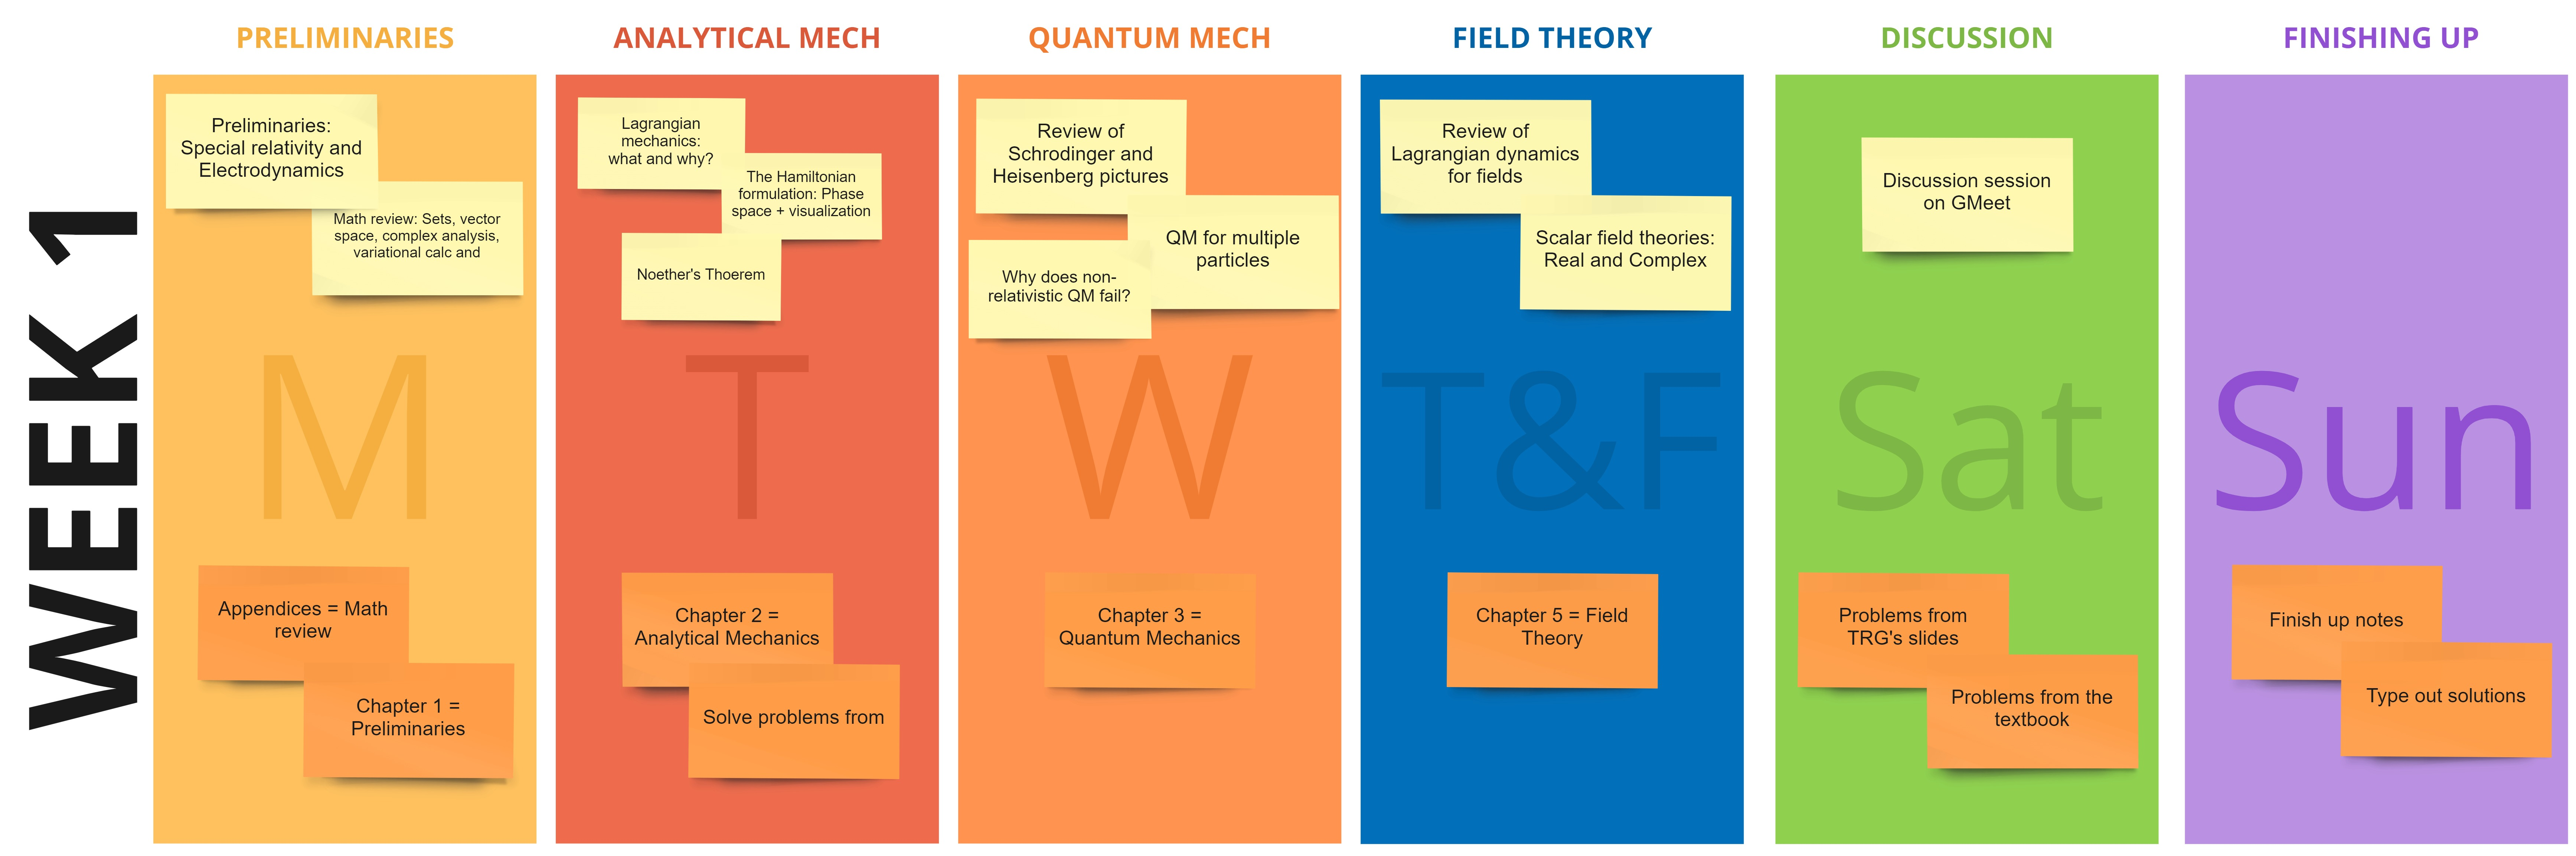
\includegraphics[scale=0.095]{Figures/Week1.jpg}
\end{figure}
\end{landscape}


\begin{savequote}[45mm]
The Theory of Relativity confers an absolute meaning on a magnitude which in classical theory has only a relative significance: the velocity of light. The velocity of light is to the Theory of Relativity as the elementary quantum of action is to the Quantum Theory: it is its absolute core.  
\qauthor{Max Planck}
\end{savequote}
\chapter{Preliminaries}
\label{ch:preliminaries}
\section{Special Relativity}
\begin{tcolorbox}
    Need for Special Relativity
\end{tcolorbox}
\begin{itemize}
    \item Newtonian Mechanics only seem to be relevant in certain frames of reference called as inertial frames of reference and all inertial frames of references are equivalent to each other. When we take up the case of Maxwell's theory of Electromagnetism, it was observed that there exists a set of preferred frames of references which goes against the understanding of the Galilean relativity. Hence to join the dots, Einstein formulated the theory of Special relativity which gives distinguished properties to individual frames of references wherein the speed of light is the only parameter that remains constant in all frames of reference.
    \item According to Special Relativity, the frames of reference are 4 dimensional. They are the spatial co-ordinate axes(x,y,z) and the time axis (t) and hence was termed as Space-time.
    \item Objects or "points" in a frame move along space and time and thus indicates that the events occurring in one frame need not occur in another frame at the same time.
    \item The points on a frame can be viewed on another frame of reference using some transformation laws. These transformation laws are called as Lorentz Transformation.
\end{itemize}
\subsection{Spacetime}
The distance between any two points in space is given by, 
\begin{equation}
    \Delta s^{2} = (\Delta x^{1})^{2} + (\Delta x^{2})^{2} + (\Delta x^{3})^{2} = \sum_{i=1}^{3}(\Delta x^{i})^{2}
\end{equation}
We can choose a new set of Cartesian axes and still the distance between the two points remain unchanged. 
\begin{equation}
\Delta s^{2} = \sum_{i=1}^{3}(\Delta x^{i^{1}})^{2}
\end{equation}
where the new set of axis is denoted by $x^{i^{1}}$. 
If the rotation between the axes is given by an angle $\theta$, we can  relate $x^{i}$ and $x^{i^{1}}$ by the equation, 
\begin{equation}
x^{i^{1}} = \Lambda ^{i^{1}} x^{i}_{i} =  \sum_{i=1}^{3} \Lambda ^{i^{1}} x^{i}_{i}
\end{equation}
\begin{equation}
x^{i^{1}} = \Lambda ^{i^{1}} x^{i}_{i}
\end{equation}
where, 
\begin{equation}
\Lambda ^{i^{1}} = \begin{pmatrix}
\cos \theta & \sin \theta & 0\\
-\sin \theta & \cos \theta & 0 \\
0 & 0 & 1
\end{pmatrix}
\end{equation}
Equation (1.4) gives the expression for Lorentz invariance.\\ 
In ordinary Newtonian physics, if one uses Cartesian coordinates, these are all the vector transformations one needs where the time variable 't' remains unchanged. \\
But it is not the case in Special Relativity. Special relativity refers to space-time and involves transformations that mix spacial co-ordinates and time co-ordinates together. 
\subsection{Minkowski Metric}
\begin{tcolorbox}
  \begin{equation}
     \Delta s^{2} = (c \Delta t)^{2} + (\Delta x^{1})^{2} + (\Delta x^{2})^{2} + (\Delta x^{3})^{2}
  \end{equation}
\end{tcolorbox}
The zeroth component in $x^{\mu}$ with $\mu = 0,1,2,3$ is the time component wherein it is expressed as 'ct' to keep the units of all the components same.Generally we take "c=1" to measure time in terms of distance. \\
The Lorentz invariant is given by, 
\begin{equation}
x^{\mu^{1}} = \Lambda ^{\mu ^{1}} x_{\mu} ^{\mu}
\end{equation}
For a rotation of the frame by an angle of $\theta$, we have the 
\begin{equation}
    \Lambda ^{\mu ^{1}}_{\mu} =  \begin{pmatrix}
1 & 0 & 0 & 0 \\
0 & \cos \theta & \sin \theta & 0\\
0 & -\sin \theta & \cos \theta & 0 \\
0 & 0 & 0 & 1 \\
\end{pmatrix}
\end{equation}
if we change to a coordinate system that is moving along the $x^{1}$ direction
with velocity v with respect to the original one, we have
\begin{equation}
    \Lambda ^{\mu ^{1}} _{\mu}  =  \begin{pmatrix}
\cos \phi & -\sin \phi & 0 & 0\\
-\sin \phi & \cos \phi & 0 & 0 \\
0 & 0 & 1 & 0 \\
0 & 0 & 0 & 1 \\
\end{pmatrix}
\end{equation}
where $\phi = tanh^{-1}(v) $ \\ 
Using the above expression, 
\begin{equation}
t^{1} = \gamma (t-vx)
\end{equation}
\begin{equation}
    x^{1} = \gamma (x-vt)
\end{equation} 
Where $\gamma = \frac{1}{\sqrt{1-v^{2}/c^{2}}}$ 
\subsection{Space-like, Time-like and Light-like}
\begin{tcolorbox}
\begin{itemize}
    \item At every point in space-time there is a future and past light cone 
    \item All points within the future or past light cones of a given point are said to be time-like separated with respect to a reference point and the space-time distance between those points is negative.
    \item Points outside the light cone are space-like separated and their distance to the origin is positive. 
    \item The points along the light cone are light-like or null separated and their distance to the origin is zero. 
\end{itemize}
 \end{tcolorbox}
 \subsection{Relativistic Mechanics}
 The proper length between two points in space-time is given by, 
 \begin{tcolorbox}
 \begin{equation}
    \Delta l = \int \sqrt{\eta_{{\mu}{\nu}} \frac{\delta x^{\mu}}{\delta \lambda} \frac{\delta x^{\nu}}{\delta \lambda} }\delta \lambda
 \end{equation}
 \end{tcolorbox}
 where $\lambda$ is a parameter of $x^{\mu}$ and ,
 \begin{equation*}
     \eta _{{\mu}{\nu}} = \Lambda_{\mu}^{\mu^{1}} \Lambda_{\nu}^{\nu^{1}} \eta _{{\mu^{1}}{\nu}^{1}}
 \end{equation*}
 The proper time for two events occurring at two different points in space-time is given by, 
 \begin{tcolorbox}
 \begin{equation}
  \Delta T = \int \sqrt{-\eta_{{\mu}{\nu}} \frac{\delta x^{\mu}}{\delta \lambda} \frac{\delta x^{\nu}}{\delta \lambda} }\delta \lambda
  \end{equation}
 \end{tcolorbox}
 The reason for the negative sign is that if we consider a space-time trajectory that does not move spatially, that is a particle at rest, then $\Delta T = \Delta t$ which is time measured at rest, with respect to the particle. Particle trajectories are always time-like or, if one considers massless particles, null. In that case the length of the trajectory disappears.
 \subsection{Raising and Lowering Indices}
 In space-time it is useful to make a distinction between sub-indices and super-indices. \\
 The four vectors $\eta_{\mu}^{\nu}$ and  $\eta_{\nu}^{\mu}$ are not one and the same. \\
 We can define the four vectors with different indices with the expression, 
 \begin{equation}
  \eta_{\mu} = \Lambda^{{\mu}{\nu}} \eta^{\nu}
 \end{equation}
 and for the other case, 
 \begin{equation}
     \eta^{\mu} = \Lambda_{{\mu}{\nu}} \eta_{\nu}
 \end{equation}
 This is called lowering or raising indices which will prove essential for formulating the expressions for various other four vectors. 
 \section{An example: Compton Effect}
 
 Lets try applying the four vector formulism to a very renowned formula based on Compton effect. \\
 The 4-momentum of a particle is given by ,
 \begin{equation}
    P \equiv (P_{0}, P_{1}, P_{3}, P_{4}) \equiv (E, P_{x}c, P_{y}c, P_{z}c) \equiv (E, pc)
 \end{equation}
 The square of a 4-momentum that is, the inner product of a 4-momentum with
itself is therefore,
\begin{equation}
    P^{2} \equiv P . P \equiv E^{2} - |P|^{2}c^{2}= m^{2}c^{4}
\end{equation}
Since momentum in conserved, the initial momentum is equal to the momentum after collision. $P_{initial}= P_{final}$ \\

The 4-Momenta before the collision is given by,
\begin{equation}
    P_{initial} = (\frac{hc}{\lambda}, \frac{hc}{\lambda}, 0, 0) , \: P_{m} = (mc^{2}, 0, 0, 0)
\end{equation}
The 4-Momenta before the collision is given by,
\begin{equation}
   P_{final} = (\frac{hc}{\lambda^{1}}, \frac{hc}{\lambda^{1}} \cos{\theta}, \frac{hc}{\lambda^{1}} \sin{\theta}, 0) 
\end{equation}
 
 \begin{figure}
    \centering
    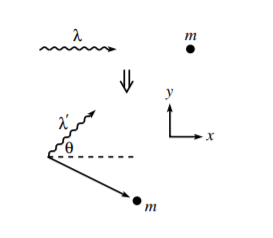
\includegraphics{Figures/compton effect .png}
    \caption{Compton Scattering}
    \label{fig:my_label}
\end{figure}
From the law of conservation of momentum and energy,  we get, 
\begin{eqnarray}
P_{initial} + P_{m} = P_{final}+ P_{m}^{1} \\
(P_{initial} + P_{m}- P_{final})^{2}  = (P_{m}^{1})^{2} \\
P_{initial}^{2} + P_{m}^{2}+ P_{final}^{2} + 2 P_{m}(P_{initial} - P_{final} )- 2 P_{initial}P_{final} = (P_{m}^{1})^{2} \\
0+ m^{2}c^{4} + 0 + 2m c^{2}(\frac{hc}{\lambda} -\frac{hc}{\lambda^{1}}) - 2 \frac{hc}{\lambda} \frac{hc}{\lambda^{1}} (1-\cos{\theta}) = m^{2}c^{4}
\end{eqnarray}
Multiplying throughout by $(\frac{\lambda \lambda^{1}}{2hmc^{3}})$ f=gives, 
\begin{equation}
    \lambda^{1} = \lambda + \frac{h}{mc}(1- \cos{\theta})
\end{equation}
\begin{itemize}
    \item If $\theta \approx 0$, then $\lambda \approx \lambda^{1}$
    \item if $\\theta = \pi $ and $\lambda << \frac{h}{mc} $ then, $\lambda^{1}= \frac{2h}{mc}$, so, 
    \begin{equation}
    E_{final}=\frac{hc}{\lambda} \approx \frac{\frac{hc}{2h}}{mc} = \frac{1}{2}mc^{2}
    \end{equation}
    That is to say that the photon bounces back with a certain $E_{final}$ which is independent of $E_{initial}$. 
\end{itemize}



\begin{savequote}[45mm]
When I was in high school, my physics teacher called me down one day after
class and said, "You look bored, I want to tell you something interesting".
Then he told me something I have always found fascinating. Every time
the subject comes up I work on it.  
\qauthor{Richard Feynman}
\end{savequote}
\chapter{Analytical Mechanics}
\label{ch:method}
\section{Lagrangian Mechanics}
\begin{tcolorbox}
In the formulation of Lagrangian mechanics, we have the action functional
\begin{equation}
    S = \int^{b}_{a} L(x^{\mu}, {{x}^{'}}^{\mu}, t) \ dt
\end{equation}
the equations of motion are obtained when we stationarize the the action i.e. when we equate the Frechet derivative of the Lagrangian to . This produces $n$ $2^{\text{nd}}$ order non-linear (in most cases) partial differential equations. And generally for non-dissipative systems
\begin{equation}
    L = T - V
\end{equation}
Where $T$ is the kinetic energy of the system and $V$ the potential energy
\end{tcolorbox}
The advantages of using the Lagrangian mechanics are:
\begin{itemize}
    \item Scalars are used instead of vectors which makes calculations much easier
    \item The concept of forces is discarded and thus only knowledge of the kinetic and potential energy is required 
    \item Generalized coordinates are used thus, it is easier to transform to any arbitrary coordinate system (composed of only independent coordinates)
    \item Lagrangian mechanics holds for all frames of references, not just inertial frames
\end{itemize}
One key point however is that when we are talking about Lagrangian mechanics, we are not exactly talking about but rather a representation of it as the space of the arguments of the lagrangian for a system with $n$ independent coordinates lives in a $3n$ dimensional space called the configuration space
\begin{figure}[H]
    \centering
    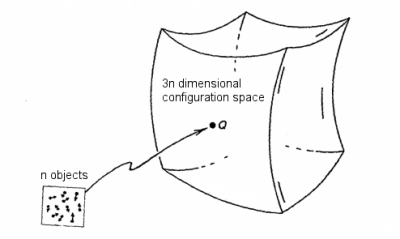
\includegraphics[scale=0.5]{Figures/configspace.png}
    \caption{A visualization of configuration space}
    \label{fig:my_label}
\end{figure}
\subsection{Constraints}
Holonomic constraints are relationships between the coordinates of the form
    \begin{align}
        f_{\alpha}(x^{\mu},t) = 0 \ \ , \ \ \alpha = 1,..,3N-n
    \end{align}
Holonomic constraints can be solved in terms of $n$ generalized coordinates $q_{i}$ where $i$ runs from $1$ to $n$. So 
\begin{equation}
    x^{\mu} = x^{\mu}(q_{1},..,q_{n})
\end{equation}
The system is said to have $n$ degrees of freedom. Let's take a look at an example
\begin{figure}[H]
    \centering
    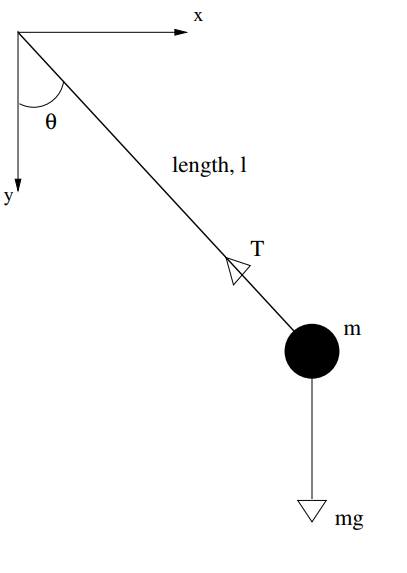
\includegraphics[scale=0.5]{Figures/pendulum.png}
    \caption{A Simple Pendulum}
    \label{fig:my_label}
\end{figure}
here the pendulum has a single degree of freedom, $q = \theta$. We have the equations of motion
    \begin{align}
        m\ddot{x} = -Tx/l \ \ , \ \ m \ddot{y} = mg - Ty/l
    \end{align}
and constraints
    \begin{align}
        \ddot{\theta} = -(g/l)sin(\theta) \ \ , \ \  T = ml\dot{\theta}^{2} + mg cos(\theta)
    \end{align}
Now let's see how we can solve this using the Lagrangian formalism. We start by introducing $3N-n$ new variables $\lambda_{\alpha}$, called Lagrange multipliers and define a new Lagrangian
\begin{equation}
    L^{'} = L(x^{\mu},\dot{x}^{\mu}) + \lambda_{\alpha} f_{\alpha}(x^{\mu},t)
\end{equation}
We treat $\lambda_{\alpha}$ like new coordinates. Since $L^{'}$ doesn't depend on $\dot{\lambda}_{\alpha}$, thus the Euler-Lagrange equations for $\lambda_{\alpha}$:
\begin{equation}
    \frac{\partial L^{'}}{\partial \lambda_{\alpha}} = f_{\alpha}(x^{\mu},t) = 0
\end{equation}
and the equations for the $x^{\mu}$ are
\begin{equation}
    \frac{d}{dt}\left( \frac{\partial L}{\partial \dot{x}^{\mu}} \right) - \frac{\partial L}{\partial x^{\mu}} = \lambda_{\alpha} \frac{\partial f_{\alpha}}{\partial x^{\mu}}
\end{equation}
Here the RHS represents the constrained system's equation of motion and the LHS the unconstrained one.
Let's have one more go at this problem, the Lagrangian for the pendulum is given by a free particle moving in a plane i.e. a circle
\begin{equation}
    L^{'} = \frac{1}{2}m(\dot{x}^{2} + \dot{y}^{2}) + mgy + \frac{1}{2}\lambda(x^{2} + y^{2} - l^{2})
\end{equation}
from which we get the equations of motion for $x$ and $y$,
\begin{equation}
    m \ddot{x} = \lambda x
\end{equation}
\begin{tcolorbox}
    \textbf{Theorem:} For constrained systems we may derive the equations directly in terms of the generalized coordinates $q_{i}$
    \begin{equation}
        L(q^{i},\dot{q}^{i}, t) = L(x^{\mu}(q^{i},t),\dot{x}^{\mu}(\dot{q}^{i}, t))
    \end{equation}
    \textbf{Proof:} Let's work with $L^{'} = L + \lambda_{\alpha}f_{\alpha}$ and change coordinates to:
    \begin{equation}
    x^{\mu} \rightarrow 
        \begin{cases}
            q_{i} \ \ \ & i = 1,...,n\\
f_{\alpha},            \ \ \  & \alpha = 1,...,3N-n
        \end{cases}
    \end{equation}
    We know that Lagrange's equations take the same form in these new coordinates
    \begin{equation}
        \frac{d}{dt}\left( \frac{\partial L}{\partial \dot{q}^{i}} \right) - \frac{\partial L}{\partial q^{i}} = \lambda_{\alpha} \frac{\partial f_{\alpha}}{\partial q^{i}}
    \end{equation}
    But, by definition $\partial f/\partial q_{i} = 0$, thus we are left with Lagrange's equations purely in terms of the generalized coordinates with no sign of constraint forces. Therefore, if we are only interested in the dynamics of generalized coordinates, we may ignore the Lagrange multipliers and simply work with the unconstrained Lagrangian.
\end{tcolorbox}
Let's look at the pendulum again. We can parameterise the constraints in terms of the generalised coordinate $\theta$ so that $x = l sin(\theta)$ and $y = l cos(\theta)$. Thus, the Lagrangian becomes
\begin{equation}
    L  = \frac{1}{2}ml^{2}\dot{\theta}^{2} + mgl cos(\theta)
\end{equation}
from this we can derive our equations of motion by means of the Euler-Lagrange equation
\begin{equation}
    \frac{d}{dt}\left(\frac{\partial L}{\partial \dot{\theta}}\right) - \frac{\parital L}{\partial \theta} = ml^{2}\ddot{\theta} + mgl sin(\theta) = 0
\end{equation}
This indeed produces the known SHO equation.    However, it lacks the cacluability for the tension $T$.
\section{Hamilton's Mechanics}
Hamilton's equations are written as,
\begin{tcolorbox}
	\begin{equation}
\dot{q}_{i} = \frac{\partial H}{\partial p_{i}}
\end{equation}
\begin{equation}
-\dot{p}_{i} = \frac{\partial H}{\partial q_{i}}
\end{equation}
\end{tcolorbox}
	
	Where,
	$$H = T + V = \sum_{i = 1}^{n} p_{i}q_{i} - \mathcal{L}$$
	$$P = \frac{\partial \mathcal{L}}{\partial \dot{q}}$$
\subsection{Modified Hamilton's Principle}
We can thus modify Hamilton's principle to incorporate the Hamiltonian as,
\begin{equation}
\delta \int_{t_{1}}^{t_{2}} \left(\sum_{i = 1}^{n} p_{i}q_{i} - H \right) dt = 0 
\end{equation}
\subsection{Poisson Brackets}
We define Poisson Brackets as,
		\begin{equation}
		\{A, B\} = \sum_{i}^{n} \left( \frac{\partial A}{\partial q_{i}} \frac{\partial B}{\partial p_{i}} -  \frac{\partial B}{\partial q_{i}} \frac{\partial A}{\partial p_{i}}\right)
		\end{equation}
		They have the following properties,
		\begin{itemize}
		\item \textbf{Antisymmetry:} $\{A, C\} = -  \{C, A\}$
		\item \textbf{Bilinearity:} $\{kA, C\} = k \{A, C\}$
		\item $\{\left(AB\right), C\} = B\{A,C\} + A\{B,C\}$
		\end{itemize}
		
		We can rewrite Hamilton's equations through Poisson Brackets as,
		\begin{equation}
		\dot{p}_{i} = \{p_{i}, H\}
		\end{equation}
		\begin{equation}
		\dot{q}_{i} = \{q_{i}, H\}
		\end{equation}
		\begin{equation}
			\{q_{i}, p_{j}\} = \delta_{ij}
		\end{equation}
		\subsection{Arriving at the Hamiltonian equations}
		We define the Hamiltonian to be the Legendre transform of the Lagrangian with respect to the $q_{i}$ variables. We shall arrive at the Hamiltonian formalism by understanding the dynamics of the particles in the phase space. 
		\begin{equation}
		    H(q_{i}, p_{i}, t) = \sum_{i=1}^{n} p_{i} \dot{q_{i}} - L(q_{i}, \dot{q_{i}}, t)
		\end{equation}
		In terms of $p_{i}$, 
		\begin{equation}
		    p_{i} = \frac{\delta L}{\delta \dot{q_{i}}} = p_{i}(q_{j},\dot{q_{j}}, t)
		\end{equation}
		for, $\dot{q_{i}} = \dot{q_{i}}(q_{j}, p_{j},t )$ , the Hamiltonian changes to, 
	\begin{gather}
	     dH = (dp_{i} \: \dot{q_{i}}+ p_{i}d \: \dot{q_{i}}) - (\frac{\delta L}{\delta q_{i}} d q_{i} +  \frac{\delta L}{\delta \dot{q_{i}}} d\dot{ q_{i}} + \frac{\delta L}{\delta t} dt) \\ 
		    = d p_{i} \dot{q_{i}} - \frac{\delta L}{\delta q_{i}} dq_{i} - \frac{\delta L}{\delta t} dt 
	\end{gather}
	This can be re-written as, 
	\begin{equation}
	    	dH = \frac{\delta H}{\delta q_{i}} d q_{i} +  \frac{\delta H}{\delta {p_{i}}} d { p_{i}} + \frac{\delta H}{\delta t} dt
	\end{equation}
	Now we introduce the Lagrange equations which is, $\dot{q_{i}} = \frac{\delta L}{\delta q_{i}}$
\begin{tcolorbox}
    

	\begin{gather}
	    \dot{p_{i}} = - \frac{\delta H}{\delta q_{i}} \\
	    \dot{q_{i}} = \frac{\delta H}{\delta p_{i}} \\
	    - \frac{\delta L}{\delta t} = \frac{\delta H}{\delta t}
	\end{gather}
	\end{tcolorbox}
	\subsection{Examples}
	Now lets look at a few examples, 
    \begin{tcolorbox}
    \textbf{1) Particle in a potential}
    \\
            The Lagrangian for a particle moving in a 3-dimensional space is given by, 
            \begin{equation}
            L = \frac{1}{2} m \dot{r}^{2} - V(r)
            \end{equation} 
            
            By taking the derivative of the Lagrangian with respect to r, we get the momentum ,
            \begin{equation}
                P = \frac{\delta L}{\delta \dot{r}} = m \dot{r} 
            \end{equation}
            The Hamiltonian is given by , 
            \begin{equation}
                H = p \cdot \dot{r} - L = \frac{1}{2m} p^{2} + V(r)
            \end{equation}
            \begin{equation}
                \dot{r} = \frac{\delta H}{\delta p} = \frac{1}{m}p
            \end{equation}
 We have written the Hamiltonians as a function of p and r. The Hamiltonian equations are simply, 
            \begin{equation}
           \dot{p} = - \frac{\delta H}{\delta r} = - \nabla V
            \end{equation}
        The first is the definition of momentum in terms of velocity \\
        The second is Newton's equation for this system.
    \end{tcolorbox}
\begin{tcolorbox}
    \textbf{2) Particle in an electromagnetic field} \\
    The Lagrangian for a particle moving in an electromagnetic field is given by, 
    \begin{equation}
        L = \frac{1}{2} m \dot{r}^{2} - e(\phi - \dot{r} \cdot A)
    \end{equation}
    Where A is a vector potential. \\ 
    The momentum conjugate from this equation is , 
    \begin{equation}
        p = \frac{\delta L}{\delta r} = m \dot{r} + eA
    \end{equation}
    \begin{equation}
        \dot{r} = \frac{1}{m} (p - eA)
    \end{equation}
    The Hamiltonian is calculated to be, 
    \begin{gather}
        H(p,r) = p \cdot r - L
        = \frac{1}{m} p \cdot (p - eA) - [\frac{1}{2m} (p-eA)^{2}- e \phi + \frac{e}{m} (p - eA) \cdot A]
    \end{gather}
    The Hamiltonian equations become, 
    \begin{equation}
        \dot{r} = \frac{\delta H}{\delta p} = \frac{1}{m} (p-eA)
    \end{equation}
    we know $\dot{p} = -\frac{\delta H}{\delta r}$. Hence, 
    \begin{equation}
        \dot{p_{a}} = - \frac{\delta H}{\delta r_{a}} = -e\frac{\delta \phi}{\delta r_{a}} + \frac{e}{m} (p_{b}- eA_{b})\frac{\delta A_{b}}{\delta r_{a}}
    \end{equation}
    Hence we have the Hamiltonian equations for a particle in an electromagnetic field.  
\end{tcolorbox}
	   
	
	  
		    	
		
		
		
\section{Noether's Theorem}
Noether's Theorem essentially connects symmetries to conserved quantities, formally we can state this as:
\begin{tcolorbox}
    If the functional,
    \begin{equation}
        S = \int_{a}^{b}L(t,q^{\mu},{q^{'}}^{\mu})
    \end{equation}
    is symmetric i.e.\footnote{where $\epsilon << 1$ is a small parameter and $F$ is a scalar function}
    \begin{equation}
        L - L^{'} = \epsilon \frac{dF}{dt} + O(\epsilon^{s})
    \end{equation}
     under transformations generated by two one parameter Lie groups with the generators $\xi$ and $\tau$, then the following conservation law holds
    \begin{equation}
            p^{\mu}\xi - \mathcal{H}\tau - F = 0
    \end{equation}
    The RHS is termed the Noether current of the Lagrangian
\end{tcolorbox}
\subsection{An Example}
\begin{tcolorbox}
    \textbf{Problem:} \\
    For a change in the Lagrangian $L^{'} - L = \delta L = 0 $ under the transformation $q_{i} \rightarrow q_{i} + \delta q_{i}$ then the quantity
    \begin{equation}
        \left(\frac{\partial L}{\partial \dot{q}_{i}}\right) \delta q_{i}
    \end{equation}
    will be conserved i.e. it's first derivative w.r.t time is zero \\
    \textbf{Solution:}
For $\delta L$ we have:
\begin{equation}
    \delta L = \sum_{i} \frac{\partial L}{\partial q}\delta q_{i} + \frac{\partial L}{\partial \dot{q}} \delta \dot{q} = 0
\end{equation}
But we only have considered transformations that are not explicit or implicit functions of time, therefore we have
\begin{equation}
    \delta \dot{q}_{i} = \delta \frac{d q_{i}}{dt} = \delta \frac{d q_{i}}{dt} = 0 
\end{equation}
Therefore the variation of the Lagrangian becomes,
\begin{equation}
    \delta L =  \sum_{i} \frac{\partial L}{\partial q_{i}} \delta q_{i} = 0
\end{equation}
Since each of the generalised coordinates undergo indpendent displacements, $\delta L$ must vanish for each term of $\partial_{q_{i}}L$
\begin{equation}
    \frac{\partial L}{\partial q_{i}} = 0
\end{equation}
Plugging this into the Euler-Lagrange equation, we can see that
\begin{equation}
    \frac{d}{dt} \left( \frac{\partial L}{\partial \dot{q}_{i}} \right) = 0 \Rightarrow \frac{\partial L}{\partial \dot{q}_{i}} = \text{Constant}
\end{equation}
This quantity is constant and thus conserved. For each type of transformation of generalised coordinates that leaves the Lagrangian invariant, there will exist a conserved quantity
\end{tcolorbox}
\subsection{A Summary of Symmetries}
We summarize the symmetries as follows
\begin{center}
\begin{tabularx}{0.99\textwidth} { 
		| >{\raggedright\arraybackslash}X 
		| >{\centering\arraybackslash}X 
		| >{\raggedleft\arraybackslash}X | }
	\hline
\textbf{Characteristic of Inertial Frame} & \textbf{Property of Lagrangian} & \textbf{Conserved Quantity} \\
	\hline
	Time homogeneous & Not an explicit function of time & Total energy \\
	\hline
	Space homogeneous   & Invariant to translation  & Linear momentum  \\
	\hline
	Space isotropic   & Invariant to rotation  & Angular momentum  \\
	\hline
\end{tabularx}
			\end{center}
However, these are only spacetime symmetries and one can also talk about symmetries based off transformations of the fields themselves   
%\section{Some Niche Stuff}
%\subsection{Liouville's Theorem}
%When we consider the representative points in phase space to be sufficiently numerous that we can possibly define a density in the phase space, notably $\rho$. The volume elements of the phase space defining the density must be sufficiently large to contain a large number of representative points, but they must also be sufficiently small so that the density varies continuously.\\
%Hence he number N of systems whose representative points lie within a volume $dv$ of phase space is/
%\begin{equation}
 %   N=\rho dv
%\end{equation}
%Where,
%\begin{equation*}
    %dv=dq_1dq_2...dq_sdp_1dp_2...dp_s
%\end{equation*}
%The number of degrees of freedom of each system is s.
%Now consider an element of area in the $q_k-p_k$ plane in phase space. The number of representative points moving across the left hand edge into the area per unit time is,
%\begin{equation}
 %   \rho\frac{dq_k}{dt}dp_k=\rho\dot{q_k}dp_k
%\end{equation}
%And the number moving across the lower edge into the area per unit time is,
%\begin{equation}
 %    \rho\frac{dq_k}{dt}dp_k=\rho\dot{p_k}dq_k
%\end{equation}
%Now the total number of representative points moving into the area per unit time is,
%\begin{equation}
 %   \rho(\dot{q_k}dp_k+\dot{p_k}dq_k)
%\end{equation}
%By a Taylor series expansion, the number of representative points moving out of the area per unit time is,
%\begin{equation}
 %   \left[\rho\dot{q_k}+\frac{\partial}{\partial q_k}(\rho \dot{q_k}dq_k\right]dp_k+ \left[\rho\dot{p_k}+\frac{\partial}{\partial p_k}(\rho \dot{p_k}dp_k\right]dq_k
%\end{equation}
%The total increase in density in $dq_kdp_k$ per unit time is the difference between the two equations,
%\begin{equation}
 %   \frac{\partial_\rho}{\partial t}dq_kdp_k=-\left[\frac{\partial}{\partial q_k}(\rho \dot{q_k})+\frac{\partial}{\partial p_k}(\rho \dot{p_k})\right]dq_kdp_k
%\end{equation}
%Now, dividing by $dq_kdp_k$ and summing the expression over all possible values of $k$,
%\begin{equation}
 %   \frac{\partial \rho}{\partial t}+\sum_{k=1}^{s}\left(\frac{\partial \rho}{\partial q_k}\dot{q_k}+\rho\frac{\partial \dot{p_k}}{\partial p_k}+(\frac{\partial \rho}{\partial p_k}\dot{p_k}+\rho\frac{\partial \dot{p_k}}{\partial p_k}\right)=0
%\end{equation}
%From Hamiltons equations,
%\begin{equation*}
 %   \frac{\partial \dot{q_k}}{\partial q_k}+\frac{\partial \dot{p_k}}{\partial p_k}=0
%\end{equation*}
%So now the equation becomes,
%\begin{equation}
 %   \frac{\partial \rho}{\partial t}+\sum_{k}\left(\frac{\partial \rho}{\partial q_k}\frac{dq_k}{dt}+\frac{\partial \rho}{\partial p_k}\frac{dp_k}{dt}\right)=0
%\end{equation}
%But this is the total time derivative of $\rho$, so we conclude that,
%\begin{equation}
 %   \frac{d\rho}{dt}=0
%\end{equation}
%This is called the Liouville's theorem, and this states that the density of representative points in phase space corresponding to the motion of a system of particles remains constant during the motion.
%\subsection{Virial Theorem}
%\begin{equation}
%	S= \sum_{i}^{n} p_{i} . r_{i}
%	\end{equation}
%	\begin{equation}
%	\frac{d S}{d t} = \sum_{i}^{n} \dot{p}_{i} . r_{i} + p_{i} . \dot{r}_{i}
%	\end{equation}
	%\begin{equation}
	%\expectationvalue{\frac{d S}{d t}} = \frac{1}{\tau} \int_{0}^{r} \frac{d S}{d t} dt = \frac{S(\tau) - %S(0)}{\tau}
	%\end{equation}
	
%	\begin{equation}
%		\expectationvalue{\sum_{i}^{n} p_{i} . \dot{r}_{i}} = - \expectationvalue{\sum_{i}^{n} \dot{p}_{i} . r_{i}}
%		\end{equation}
%		\begin{equation}
%		\expectationvalue{2 \sum_{i}^{n} T_{i}} = - \expectationvalue{\sum_{i}^{n} \dot{F}_{i} . r_{i}}
%		\end{equation}
%		\begin{equation}
%		\expectationvalue{T} = - \frac{1}{2} \expectationvalue{\sum_{i}^{n} \dot{F}_{i} . r_{i}}
%		\end{equation}
%\subsection{Time Indpendent Distributions}
%\subsection{Poincare Recurrence Theorem}
%w\section{Canonical Transformations}



\begin{savequote}[45mm]
We were on a walk and somehow began to talk about space.  I had just read Weyl’s book "Space, Time and Matter", and under its influence was proud to declare that "Space was simply the field of linear operations".  ‘Nonsense,’ said Heisenberg, ‘space  is  blue and birds  fly through it.’  
\qauthor{Hermann Weyl}
\end{savequote}
\chapter{Quantum Mechanics}
\label{ch:qm}

\section{State Vector}
\begin{itemize}
\item In Quantum Mechanics, we start with an object called the state vector $\ket{\psi}$. All the information about the system is contained in it. 
\item The position basis representation of the state vector is called the wavefunction $\psi (\vec{x}, t) = \braket{x}{\psi}$.
\item If we wish to know about a particular physical measurable such as an object's position of momentum, we can extract this information from the State vector by means of acting on with an Operator that corresponds to the measurable quantity.
\end{itemize}
\subsection{Admissibility Conditions for a Wavefunction}
A physically relevant wavefunction must be:
\begin{itemize}
\item Continuous i.e. no singularities in it's topology
\item Smooth i.e. a Taylor expansion for it exists
\item Quadratically integrable with the integral being single valued i.e. finite everywhere and $\psi \rightarrow 0$ as $r \rightarrow \infty$
\item Forming an orthonormal set
\item Satisfying the boundary conditions of the quantum mechanical system it represents
\end{itemize}
\section{Observables}
\begin{itemize}
\item Observable quantities such as position and momentum.
\item Observables are represented as Hermitian operators in quantum mechanics
\end{itemize}

\section{Time Evolution}
\subsection{Schrodinger Picture}
Where\\
If we consider the Schrodinger picture i.e. the state vector evolves with time whereas the observables are in a loose sense eternal. The time evolution of the state vector is given by the Schrodinger equation:
\begin{equation}
	i \hbar \frac{\partial \ket{\psi}}{\partial t} = \hat{H} \ket{\psi}
\end{equation}
Or,
\begin{equation}
	i \hbar \frac{\partial \psi}{\partial t} = \hat{H} \psi
\end{equation}
in terms of the Wavefunction. Where, $\hat{H}$ is the Hamiltonian operator, which can be expressed as:
\begin{equation}
	\hat{H} = -\frac{\hbar^{2} \nabla^2}{2m} + V(\vec{x})
\end{equation}
for a free particle. 

\subsection{Heisenberg Picture}
In the Heisenberg picture, it is the operators which change in time while
the basis of the space remains fixed.
This is accomplished by adding a term to the Schrödinger states to eliminate the time-dependence,
\begin{equation}
    \vert \psi_H\rangle=e^{iH_st/\hbar}\vert\psi_s(t)\rangle=\vert\psi_s(0)\rangle
\end{equation}
But the operators themselves change with time,
\begin{equation}
    \hat{O}=\hat{O}(t)
\end{equation}
And they are governed by the differential equation,
\begin{equation}
    \frac{d\hat{O}}{dt}=\frac{i}{\hbar}[\hat{H}_s,\hat{O}]+ \left(\frac{\partial\hat{O}}{\partial t}\right)
\end{equation}
\section{Measurement}
Measurement is defined as a form of time-evolution that is non-unitary and non-deterministic. 
According to Born's rule
\begin{equation}
	\int_{a}^{b} \abs{\psi(\vec{x}, t)}^{2} dx = \text{Probability of finding the particle at a time t between positions a and b}
\end{equation}
Thus, . Physically speaking this lends a kind of indeterminacy to the wavefunction. We can only speak of probabilities. Therefore, we can only , this brings to the measurement hypothesis, that is the State vector evolves to the state corresponding to the measurement being made. And unlike the Schrodinger equation, this evolution is non-deterministic. This tension is often called the "measurement problem", i.e. why is the measurement of an observable a special process distinct from others? Several theories and models claim to have resolved this, but we shall save that discussion for another time. We will fully focus on understanding the theory of Quantum Mechanics in a pragmatic lens before we question its foundations (although the converse isn't necessarily a bad thing, it isn't the purpose of this manuscript however).

\section{Summary of Postulates}
\begin{enumerate}
    \item The state of a quantum system is represented by wavefunction $\psi$. All the information about the system can be found from the knowledge of $\psi$
    \item All the physical observables are represented by Hermitian operators
    \item The outcome of measurement of any physical observables are the eigenvalues of the corresponding Hermitian operators. These eigenvalues are real.
    \item Born's interpretation states that,
    \begin{equation*}
        \rho = \psi^*\psi=|\psi|^2
    \end{equation*}
    This is called the probability density, and,
    \begin{equation*}
        \int_{b}^{a}\psi^*(x,t)\psi(x,t)dx=\text{Probability of finding particle between x=a to x=b}
    \end{equation*}
    \item The expectation values of operators are given by,
    \begin{equation*}
        \langle\hat{A}\rangle=\int\psi^*A\psi dx
    \end{equation*}
    \begin{equation*}
        \langle\hat{A}\rangle=\int\int\int \psi^*A\psi dx dy dz
    \end{equation*}
    If it is not normalised,
    \begin{equation*}
        \langle \hat{A}\rangle=\frac{\int\psi^*A\psi dx}{\int\psi^*\psi}
    \end{equation*}
    \item The time evolution of the wavefunction is governed by the Schrodingers equation,
    \begin{equation*}
        i\hbar\frac{\partial \psi}{\partial t}=\hat{H}\psi
    \end{equation*}
\end{enumerate}
\section{Normalization}
Normalization is a process through which we ensure that,
\begin{equation}\label{norm}
	\int_{- \infty}^{\infty} \abs{\psi(\vec{x}, t)}^{2} dx = 1
\end{equation}
This is a natural consequence of Born's rule, we simply want all the probabilities to add up to 1. Thus, to rule out any other absurd scenarios, we make a ruling that non-Normalizable and non-square integrable Wavefunctions are unphysical.\\
We can also prove that once normalized, the wavefunction always remains normalized, we start by differentiating equation (\ref{norm}) with respect to time\\
$$\frac{d}{dt} \int_{- \infty}^{\infty} \abs{\psi(\vec{x}, t)}^{2} dx = \frac{\partial}{\partial t}\int_{- \infty}^{\infty} \abs{\psi(\vec{x}, t)}^{2} dx$$
Dealing with the term inside the integral,
$$ \frac{\partial}{\partial t}\abs{\psi(\vec{x}, t)}^{2} = \frac{\partial}{\partial t} (\psi^{*} \psi ) = \psi^{*}\frac{\partial \psi}{\partial t} + \psi\frac{\partial \psi^{*}}{\partial t}$$
Now the Schrodinger equation for a free particle reads as,
$$\frac{\partial \psi}{\partial t} = \frac{i \hbar}{2m}\frac{\partial^{2} \psi}{\partial x^{2}} - \frac{i}{\hbar}V \psi$$
Conjugating this we can see that,
$$\frac{\partial \psi^{*}}{\partial t} = -\frac{i \hbar}{2m}\frac{\partial^{2} \psi^{*}}{\partial x^{2}} + \frac{i}{\hbar}V \psi^{*}$$
Thus,
$$\frac{\partial}{\partial t}\abs{\psi(\vec{x}, t)}^{2} = \frac{i \hbar}{2m}\left( \psi^{*} \frac{\partial^{2} \psi}{\partial x^{2}} - \psi \frac{\partial^{2} \psi^{*}}{\partial x^{2}} \right) = \frac{\partial }{\partial x}\left[\frac{i \hbar}{2m}\left( \psi^{*} \frac{\partial \psi}{\partial x} - \psi \frac{\partial \psi^{*}}{\partial x} \right)\right]$$
Now we evaluate the integral,
$$\frac{d}{dt} \int_{- \infty}^{\infty} \abs{\psi(\vec{x}, t)}^{2} dx = \frac{i \hbar}{2m}\left( \psi^{*} \frac{\partial \psi}{\partial x} - \psi \frac{\partial \psi^{*}}{\partial x} \right)^{\infty}_{- \infty} $$
But $\psi$ must go to zero as goes to infinity, otherwise the wave function would not be normalizable. Thus it follows that.
\begin{equation}
	\frac{d}{dt} \int_{- \infty}^{\infty} \abs{\psi(\vec{x}, t)}^{2} dx = 0
\end{equation}
And hence, the integral is constant i.e. independent of time. Therefore if is normalized at a time $t = 0$, it remains normalized for all future. 
\section{Generalized Uncertainty Principle}
\subsection{Cauchy-Schwarz Inequality}
For all triangles as depicted above, 
$$|X| + |Y| \geq |Z|$$
Where |X| is the length of the vector $\vec{X}$. We can also write the last equation as:
$$|\vec{X}| + |\vec{Y}| \geq |\vec{X} + \vec{Y}|$$
Squaring this equation it becomes, 
$$|\vec{X}|^2 + |\vec{Y}|^2 + 2|\vec{X}||\vec{Y}| \geq |\vec{X} + \vec{Y}|^2$$
Expanding the right side we get, 
$$|\vec{X}|^2 + |\vec{Y}|^2 + 2|\vec{X}||\vec{Y}| \geq |\vec{X}|^2 + |\vec{Y}|^2 + 2(\vec{X}.\vec{Y})$$ 
Cancelling the terms we find, 
$$|\vec{X}||\vec{Y}| \geq \vec{X}.\vec{Y}$$ 
This is called the Cauchy-Schwarz inequality. Writing this using the state vectors, $$|X| = \sqrt{\langle X| X \rangle}$$
$$|Y| = \sqrt{\langle Y| Y \rangle}$$ 
$$|X + Y| = \sqrt{(\langle X | + \langle Y |)(|X\rangle + |Y\rangle)}$$ 
we have by substituting into the inequality, 
$$\sqrt{\langle X| X \rangle} + \sqrt{\langle Y | Y \rangle} \geq \sqrt{\langle X|Y \rangle + \langle Y|X \rangle}$$ 
squaring it and simplifying we find 
$$2|X||Y| \geq |\langle X|Y \rangle + \langle Y|X \rangle |$$
This is the Cauchy-Schwarz inequality written in terms of state vectors.
The Uncertainity Principle
Suppose we have a ket $| \psi \rangle$ and two operators $\hat{A}$ and $\hat{B}$, we define their standard distribution as
$$\sigma^{2}_{A} = \langle f | f \rangle$$
$$\sigma^{2}_{B} = \langle g | g \rangle$$
Where,
$$| f \rangle = (\hat{A} - \langle A \rangle)| \psi \rangle$$
$$| g \rangle = (\hat{B} - \langle A \rangle)| \psi \rangle $$
We use the Cauchy-Shwarz inequality,
$$\sigma^{2}_{A} \sigma^{2}_{B} = \langle f  | f \rangle \langle g | g \rangle \geq  {|\langle f|g \rangle|}^{2}$$
And for any complex number $z$,
$${|z|}^{2} = {[Re(z)]}^{2} + {[Im(z)]}^{2} \geq {[Im(z)]}^{2}$$
We then set, $z = \langle f | g \rangle$
$$\sigma^{2}_{A} \sigma^{2}_{B} = {\left(\frac{1}{2i} [ \langle f | g \rangle - \langle g | f \rangle]\right)}^{2}$$
But
$$\langle f | g \rangle = \langle \psi | ( \hat{A} - \langle A \rangle ) (\hat{B} - \langle B \rangle) | \psi \rangle$$
$$\langle f | g \rangle = \langle \hat{A}\hat{B} \rangle - \langle \hat{B} \rangle \langle \hat{A} \rangle - \langle \hat{A} \rangle \langle \hat{B} \rangle + \langle \hat{A} \rangle \langle \hat{B} \rangle$$
$$\langle f | g \rangle = \langle \hat{A}\hat{B} \rangle - \langle \hat{B} \rangle \langle \hat{A} \rangle - \langle \hat{A} \rangle \langle \hat{B} \rangle + \langle \hat{A} \rangle \langle \hat{B} \rangle$$
$$\langle f | g \rangle = \langle \hat{A}\hat{B} \rangle - \langle \hat{A} \rangle \langle \hat{B} \rangle$$
Therefore,
$$\langle g | f \rangle = \langle \hat{B}\hat{A} \rangle - \langle \hat{A} \rangle \langle \hat{B} \rangle$$
We can then say that,
$$\langle f | g \rangle - \langle g | f \rangle = \langle \hat{A}\hat{B}\rangle -  \langle \hat{B}\hat{A}\rangle= \langle \psi | \hat{A}\hat{B} - \hat{B}\hat{A} | \psi \rangle$$
Which is the same as,
$$\langle f | g \rangle - \langle g | f \rangle = \langle [\hat{A},\hat{B}] \rangle$$
Putting this all together we get,
$$\sigma^{2}_{A} \sigma^{2}_{B} \geq {\left(\frac{1}{2i}\langle [\hat{A},\hat{B}] \rangle\right)}^{2}$$
This is called the generalized uncertainty principle. This basically states that two variables that do not commute cannot be measured with precision simultaneously. 
Talking about position and momentum
We know that observable properties can be represented using operators, here we'll
$$\hat{x} = x$$
$$\hat{P} = -i\hbar \frac{\partial}{\partial x}$$
So we now try to find the commutator of those operators now
$$[\hat{x}, \hat{p}] = \hat{x}\hat{p} - \hat{p}\hat{x}$$
$$[\hat{x}, \hat{p}] = -ix\hbar \frac{\partial}{\partial x} + i\hbar \frac{\partial}{\partial x}$$
Now let's apply this to state vector to obtain the expectation value 
$$[\hat{x}, \hat{p}] |\psi\rangle = -ix\hbar \frac{\partial}{\partial x} |\psi\rangle + i\hbar \frac{\partial x|\psi\rangle}{\partial x}$$ 
$$[\hat{x}, \hat{p}] |\psi\rangle = -ix\hbar \frac{\partial}{\partial x} |\psi\rangle + ix\hbar \frac{\partial |\psi\rangle}{\partial x} + i\hbar$$
$$[\hat{x}, \hat{p}] |\psi\rangle = i\hbar$$
Substituting this into the generalized uncertainty principle,
$$\sigma_{x}\sigma_{p} \geq \frac{1}{2i} i\hbar$$
$$\sigma_{x}\sigma_{p} \geq \frac{\hbar}{2} $$
$$\sigma_{x}\sigma_{p} \geq \frac{h}{4 \pi}$$
\subsection{Summary}
We can visualize all of this in the form of waves. The more precisely we measure its wavelength
image
the less precisely we measure its frequency.
image
Thus, the state vector can be thought of a wave whose frequency and wavelength somehow correspond to position and momentum or it is simply a wave in a space where the axes are position and momentum. The uncertainty principle thus isn't just a property of quantum Mechanics but is a property of waves in general.
\section{Stationary State}
A  stationary state $\psi_{0}$ is a quantum mechanical state:
\begin{itemize}
\item with all observables independent of time
\item an eigenvector of the Hamiltonian
\item corresponds to a state with a single definite energy
\end{itemize}
Stationary states themselves are not constant in time but their probability densities $\abs{\psi_{0}}^{2}$ are
\section{The Continuity Equation}
\begin{tcolorbox}
\begin{equation}
\frac{\partial \rho}{\partial t} = - \nabla . \vec{J}
\end{equation}
\end{tcolorbox}
Where,
$$\rho = \psi \psi^{*}$$
$$\vec{J} = \frac{\hbar}{2mi} \left[ \psi^{*} \nabla \psi - (\nabla \psi^{*})\psi\right]$$

\subsection{Interpretation}
\begin{itemize}
\item Probability is conserved i.e. $\sum_{i}^{\infty}P_{i} = 1$ \footnote{This holds well in the non-relativistic case i.e. when there is no creation or annihilation of particles}
\item The probability density evolves deterministically
\end{itemize}
\section{Toy Models}
\subsection{Infinite Square Well}
The Schrodinger equation is given by,
\begin{equation}
	-\frac{\hbar^2}{2m}\frac{d^2\psi}{dx^2}=E\psi
\end{equation}
And so,
\begin{equation}
	\frac{d^2\psi}{dx^2}=k^2\psi \; \text{where}\, k\equiv\frac{\sqrt{2mE}}{\hbar}
\end{equation}
This equation is simply the simple harmonic oscillator equation, whose general solution is,	\begin{equation}
	\psi(x)=A\sin kx + B\cos kx
\end{equation}
Continuity of $\psi(x)$ requires that,
	\begin{equation*}
		\psi(0)=\psi(a)=0
	\end{equation*}
		This is called the boundary conditions for our problem at hand. Now imposing this on A and B,
		\begin{equation}
			\psi(0)=A\sin 0 + B\cos 0 =B
		\end{equation}
		So $B=0$, and hence,
		\begin{equation}
			\psi(x)=A\sin kx
		\end{equation}
		Then, $\psi(a)=A\sin ka$, so $\sin ka=0$, which means that,
		\begin{equation}
			ka=0, \; \pm\pi, \; \pm2\pi, \; \pm3\pi...
		\end{equation}
			Negative solutions are insignificant, so the distinct solutions are,
		\begin{equation}
			k_n=\frac{n\pi}{a}, \, \text{with}\; n=1,2,3,...
		\end{equation}
	And so the possible values (eigenvalues) of $E$ are,
	\begin{equation}
		E_n=\frac{\hbar^2k^2_n}{2m}=\frac{n^2\pi^2\hbar^2}{2ma^2}
	\end{equation}
		Finding A using by normalisation,
	\begin{equation}
		\int_{0}^{a}|A|^2\sin^2(kx)dx=|A|^2\frac{a}{2}=1 \, \text{so} \, |A|^2=\frac{2}{a}
	\end{equation}
	Now the eigenfunction is,
	\begin{equation}
		\psi_n(x)=\sqrt{\frac{2}{a}}\sin \left(\frac{n\pi}{a}x\right)
	\end{equation}
	
	\subsection{The Harmonic Oscillator }
		For a harmonic oscillator, we try to solve the Schrodinger equation with the potential,
			\begin{equation}
				V(x)\frac{1}{2}m\omega^2x^2
			\end{equation}
			And so,
			\begin{equation}
				-\frac{\hbar}{2m}\frac{d^2\psi}{dx^2}+\frac{1}{2}m\omega^2x^2\psi=E\psi
			\end{equation}
			Writing this more neatly,
			\begin{equation}
				\frac{1}{2m}[\hat{p}^2+(m\omega x)^2]\psi=E\psi
			\end{equation}
		where $\hat{p}\equiv-i\hbar d/dx$ is the momentum operator. Here, we are simply trying to factor out the Hamiltonian,
		The Hamiltonian can be said to be,
				\begin{equation}
				\hat{H}=\frac{1}{2m}[\hat{p}^2+(m\omega x)^2]
				\end{equation}
			But we cannot factor out the Hamiltonian that easily, since the quanitites are operators and they do not commute. So we introduce a new quantity
			\begin{equation}
				\hat{a}\pm\equiv\frac{1}{\sqrt{2\hbar m\omega}}(\mp i\hat{p}+m\omega x)
			\end{equation}
		Now,
		\begin{align}
			\hat{a_-}\hat{a_+}&=\frac{1}{2\hbar m\omega}(i\hat{p}+m\omega x)(-i\hat{p}+m\omega x)\\
							  &=\frac{1}{2\hbar m\omega}[\hat{p}+(m \omega x)^2-im\omega(x\hat{p}-\hat{p}x)]
		\end{align}
			Now, writing this using commutator brackets,
			\begin{equation}
				\hat{a_-}\hat{a_+}=\frac{1}{2\hbar m\omega}[\hat{p}^2+(m\omega x)^2]-\frac{i}{2\hbar}[x,\hat{p}]
			\end{equation}
			Using the canonical commutation relation,
			\begin{equation*}
				[x,\hat{p}]=i\hbar
			\end{equation*}
			\begin{equation}
					\hat{a_-}\hat{a_+}=\frac{1}{\hbar \omega}\hat{H}+\frac{1}{2}
			\end{equation}
			Rearranging
				\begin{equation}
					\hat{H}=\hbar\omega\left(\hat{a_-}\hat{a_+}-\frac{1}{2}\right)
				\end{equation}
					Now doing the same for the other case,
			\begin{equation}
				\hat{H}=\hbar\omega \left(\hat{a_+}\hat{a_-}+\frac{1}{2}\right)
			\end{equation}
			The Schrodinger equation can be written as,
			\begin{equation}
				\hbar\omega\left(\hat{a\pm}\hat{a\mp}\pm\frac{1}{2}\right)\psi=E\psi
			\end{equation}
			Now, we make the claim,
			\begin{gather*}
				\hat{H}\psi=E\psi \\
				\hat{H}(\hat{a_+}\psi)=(E+\hbar\omega)(\hat{a_+}\psi)
			\end{gather*}
			Applying the lowering operator to the ground state wavefunction,
			\begin{equation}
				\hat{a_-}\psi_0=0
			\end{equation}
			Now $\psi_0(x)$,
			\begin{equation}
				\frac{1}{\sqrt{2\hbar m\omega}}\left(\hbar \frac{d}{dx}+m\omega x\right)\psi(0)=0
			\end{equation}
			or,
			\begin{equation}
				\frac{d\psi_0}{dx}=-\frac{m\omega}{\hbar}\psi_0
			\end{equation}
		Solving this differential equation,
		\begin{equation}
			\int\frac{d\psi_0}{\psi_0}=-\frac{m\omega}{\hbar}\int xdx=\ln(\psi_0)=-\frac{m\omega}{2h}x^2+C
		\end{equation}
		From Equation (51),
			\begin{equation}
				\psi_0(x)=Ae^{-\frac{m\omega}{2\hbar}x^2}
			\end{equation}
			From normalisation we have,
			\begin{equation}
				A^2=\sqrt{m\omega/\pi\hbar}
			\end{equation}
			And now,
			\begin{equation}
				\psi_0(x)=\left(\frac{m\omega}{\pi\hbar}\right)^{1/4}e^{-\frac{m\omega}{2\hbar}x^2}
			\end{equation}
			Now our ground state energy is given by,
			\begin{equation}
				E_0=\frac{1}{2}\hbar\omega
			\end{equation}
				From here, we can just apply the raising operators from the ground state to obtain our excited state eigenfunctions and energies,
			\begin{gather}
				\psi_n(x)=A_n(\hat{a_+})^n\psi_0(x)\\
				E_n=\left(n+\frac{1}{2}\right)\hbar\omega
			\end{gather}
\section{Quantum Mechanical Transformations}
In this section we are going to look at how quantum states, operators and quantum fields will transform when subjected to translations, rotations or Lorentz boosts.  \\
The translation of a three-vector is achieved by adding a factor "$a$" to the vector. 
\begin{equation}
    x^{'} = T(a)x = x+a
\end{equation}
Rotation of a three vector is given by 
\begin{equation}
x^{'} = R(\theta)x =  \begin{pmatrix}
\cos \theta & -\sin \theta & 0\\
\sin \theta & \cos \theta & 0 \\
0 & 0 & 1  \\
\end{pmatrix}
\end{equation}
Let us try to formulate operators that can transform quantum mechanical states in Hilbert space. 
\subsection{Translation in Spacetime}
Lets define a quantum mechanical operator $\hat{U}$ that takes a state localized at x and transforms it to a position x+a.
\begin{equation}
    \hat{U}(a) \ket{x} = \ket{x+a}
\end{equation}
This falls under the category of active transformation wherein we move the particle to another point in the space which is contrary to the passive transformation wherein we move the axes while keeping the position of the object fixed. \\ 
Let us define some translation properties that our operator must possess. 
\begin{itemize}
    \item Our operator should not change the probability density when it acts on the state vector. 
    \begin{equation}
        \braket{\psi(x)} = \braket{\psi(x+a)} = \bra{\psi(x)}\hat{U^{\dagger}}(a) \hat{U}(a) \ket{\psi(x)}
    \end{equation}
    Which means, 
    \begin{equation}
        \hat{U^{\dagger}}(a)\hat{U}(a) = 1
    \end{equation}
    This is to say that our operator is unitary. 
    \item We want our operator to be composite, i.e, 
    \begin{equation}
        \hat{U}(a) \hat{U}(b) = \hat{U}(a+b)
    \end{equation}
    \item Just for completeness sake, we should also have the trivial property that the transformation can do nothing to the particle, that is $\hat{U}(0)= 1$
\end{itemize}
Now to put all of our conditions together, we get, 
\begin{eqnarray}
 \hat{U^{\dagger}}(a)\hat{U}(a) = 1 (Unitarity)\\
  \hat{U}(a) \hat{U}(b) = \hat{U}(a+b)(Composite) \\
  \hat{U}(0)= 1(Zero \: translation \: does \: nothing \: to \: the \: particle)
\end{eqnarray}
These translation properties of the operator suggests that it should form a group in which each element depends on the value of "a" which thereby makes it differentiable, continuous, and contain infinite number of elements. This specific group is called a $\boldsymbol{Lie}$ group. \\
\\
Now that we have an idea about the properties our transformation operator must possess, lets try to come up with an explicit operator which acts on quantum states in Hilbert space. \\
\\
Lets consider a case of a positive wave function $\psi(x)= \bra{x}\ket{P}$. Lets increment $\psi(x)$ by $\delta a$ along the x-direction. 
\begin{equation}
    \psi(x+\delta ) = \psi(x) + \frac{d \psi(x)}{d x} \delta a + .....
\end{equation}
We know that $\hat{P}=-i \frac{d}{dx}$. Hence, 
\begin{equation}
    \psi(x+\delta ) = (1+ iP \delta a) \psi (x)
\end{equation}
We say that the momentum operator $\hat{P}$ is the "generator" for the space
translation. \\
For 'N' translations, we have, 
\begin{equation}
    \psi(x+a) = \lim_{N -> \infty} (1+ iP \delta a)^{N} \psi (x)
\end{equation}
This gives us a space evolution operator.  \\
\\
The translation operator is therefore, 
\begin{equation}
    \hat{U}(a) = e^{-i\hat{P} . a}
\end{equation}
Lets look at how the operator evolves with time. Lets evolve the system by a time $\delta t_{a}$. We get, 
\begin{equation}
\psi(t+\delta t_{a}) = \psi (t) + \frac{d \psi(t)}{d t} \delta t_{a}
\end{equation}
We know that $\hat{H} = i \frac{d}{dt}$, hence, 
\begin{equation}
    \psi(t+\delta t_{a}) = (1- iH \delta t_{a}) \psi (t)
\end{equation}
To change the operator from a time evolving operator to a time translation operator, we need to change the sign. 
\begin{equation}
    \hat{U}(t_{a}) = e^{iHt_{a}}
\end{equation}
Combining the space and time translation operators, we get, 
\begin{equation}
    \hat{U}(a) = e^{ iHt_{a} -i\hat{P} . a}
\end{equation}
We chose the four -momentum operator to be $P=(\hat{H},\hat{P})$
\subsection{Rotations in Spacetime}
We specify the rotation as $R(\theta)$, where the direction of the vector $\theta$ is the axis of rotation and its magnitude is the angle. The rotation matrix acts on the operator which for example is the momentum operator, $P^{'}= R(\theta) P$. For rotations of quantum states, we consider an operator, 
\begin{equation}
    \ket{P^{'}} = \hat{U}(\theta) \ket{P} = \ket{R(\theta)P}
\end{equation}
The operator $\hat{U}(\theta)$ has the same set of properties as the translation operator as mentioned above. \\
Since $P^{'} = R(\theta)P$, $d^{3}P= d^{3}P^{'}$
\begin{equation}
   \int d^{3}P \ket{R(\theta)P} \bra{R(\theta)P} = \int d^{3}P^{'}\ket{P^{'}}\bra{P^{'}} = 1
\end{equation}
The expression for rotation can be written as, 
\begin{equation}
    \hat{U}^{\dagger}(\theta) \hat{P} \hat{U}(\theta) = R(\theta) \hat{P}
\end{equation}
Thus the momentum operator is transformed in just the same way as we would rotate a momentum vector. \\
Lets look at how the rotation operator acts on a specific axis. Lets consider the z-axis and allow the rotation operator to act on the wave function along that axis. 
\begin{equation}
\psi(\theta^{z} + \delta \theta^{z}) = \psi(\theta^{z}) + \frac{d \theta^{z}}{d \theta^{z}}\delta \theta^{z}
\end{equation}
We know that $\hat{j}^{z}= - i \frac{d}{d \theta^{z}}$ from which we see that rotations are generated by the angular momentum operator. 
\begin{equation}
    \psi(\theta^{z} + \delta \theta^{z}) = (1+i \hat{j}^{z} \delta \theta^{z}) \psi(\theta^{z})
\end{equation}
Repeating the rotations such that $N-> \infty$, we get, 
\begin{equation}
    \hat{U}(\theta)= e^{-i \hat{j}.\theta}
\end{equation}
\subsection{Representation of Transformations}
Any rotation $R(\theta)$ can be represented by a square matrix $D(\theta)$
\begin{equation}
    D(\theta) =  e^{-i j.\theta}
\end{equation}  
In this equation, J is a square matrix representation of the operator $\hat{j}$. \begin{equation}
    j^{i} = -\frac{1}{i} \frac{\delta D(\theta^{i})}{\delta \theta^{i}}|_{\theta^{i} = 0}
\end{equation}
The important point about these representations is that they all share the same underlying algebraic structure as the rotation operator. This algebra is called a Lie algebra.
\subsection{Transformation of Quantum Fields}
We’ll try to transform quantum fields by first examining a scalar field, which is an operator-valued field whose matrix elements are scalars. \\ 
There are two ways of thinking about translations operators,
\begin{itemize}
    \item Acting on states:  $\hat{U}(a) \ket{x} = \ket{x+a}$, moves a locally defined state from being localized at x to being localized at x + a.
   \item Acting on locally defined operators: $\hat{U}^{\dagger}(a) \hat{\phi(x)} \hat{U}(a)= \phi(x-a)$
\end{itemize}
These are not the same expression as in the first equation, we move from $\ket{x} -> \ket{x+a}$, in which, $\phi(x)$ doesn't act on the state as the state is being moved.  \\
In the second one, the position of the object is being moved so $\phi(x)$ yet again misses to act on the state. 
Now, let's see what will happen if we cause a translation in spacetime by a vector a, We can try out this translated operator on
a momentum eigenstate $\ket{q}$, 
\begin{eqnarray}
     \hat{U}^{\dagger}(a) \delta_{m}^{\dagger} \hat{U}(a)\ket{q} = e^{iP \cdot a} \: \delta_{m}^{\dagger} \: e^{-iP \cdot a} \ket{q} \\
      = e^{iP \cdot a} \: \delta_{m}^{\dagger}\ket{q} \: e^{-iP \cdot a} \\
      = e^{iP \cdot a} \: \ket{m,q} \: e^{-iP \cdot a} \\
      =  \ket{m,q} e^{i(m+q) \cdot a} e^{-iq \cdot a} \\
      = \ket{m,q}e^{im \cdot a}
\end{eqnarray}
So the transformed operator $\delta_{m}^{\dagger}$ still creates a state with momentum m, but the result of the transformation is an additional phase $e^{im \cdot a}$. We conclude that, 
\begin{equation}
    \hat{U}^{\dagger}(a) \delta_{m}^{\dagger} \hat{U}(a) = e^{im \cdot a} \delta_{m}^{\dagger}
\end{equation}
 It is  important to point out that if we transform a field in some
way, we generally change the point at which the field is evaluated and also its polarization as we observe a phase difference as mentioned in the above case. \\
A more generalised notation of the rotation transforms for an arbitrary field can be written as, 
\begin{equation}
    \hat{U}^{\dagger}(a) \hat{\Phi(x)} \hat{U}(a) = D(\theta) \hat{\Phi(x)} (R^{-1}(\theta)x)
\end{equation}
\subsection{Lorentz Transformations}
The same set of transformations, which we have seen above, can be applied to the Lorentz Transformation of states of quantum fields. \\
Let's consider a 4-Boost vector along x-direction, whose Lorentz transformation is given by $x^{' \mu} = \Lambda(\beta^{'})^{\mu} x_{\nu}^{\mu}$, where, 
\begin{equation}
    \Lambda(\beta^{'}) = \begin{pmatrix}
    \gamma^{'} & \beta^{'}\gamma^{'} & 0 & 0 \\
    \beta^{'}\gamma^{'} & \gamma^{'} & 0 & 0 \\
    0 & 0 & 1 & 0 \\
    0 & 0 & 0 & 1 \\
    \end{pmatrix}
\end{equation}
This transformation connects two inertial frames moving with relative speed $v = c \beta^{'}$ along x. Using the substitutions $\gamma^{'}= \cosh{\theta^{'}} , \gamma^{'}\beta^{'} = \sinh{\theta^{'}} \: and \: \tanh{\phi^{'}} = \beta^{'}$
\begin{equation}
    \Lambda(\phi^{i}) = \begin{pmatrix}
    \cosh{\theta^{'}} & \sinh{\theta^{'}} & 0 & 0 \\
    \sinh{\theta^{'}} & \cosh{\theta^{'}} & 0 & 0 \\
    0 & 0 & 1 & 0 \\
    0 & 0 & 0 & 1 \\
    \end{pmatrix}
\end{equation}
we can write a generalized Lorentz transformation matrix as, 
\begin{equation}
    D(\phi) = e^{iK \cdot \phi}
\end{equation}
The generators of the Lorentz transformations are given by ,
\begin{equation}
K^{i} = \frac{1}{i} \frac{\delta D(\phi^{i})}{\delta \theta^{i}}|_{\phi^{i} = 0}
\end{equation}
The quantum fields have to undergo Lorentz transform given by,
\begin{equation}
     \hat{U}^{\dagger}(a) \hat{\Phi(x)} \hat{U}(a) = D(\theta) \hat{\Phi(x)} (\Lambda^{-1}(\theta)x)
\end{equation}
The commutation of the generators of the Lorentz transform is given by, 
\begin{equation}
    [K^{1}, K^{2}] = K^{1}K^{2} - K^{2}K^{1} = -ij^{3}
\end{equation}
Some commutation laws of the generators of Lorentz transforms are, 
\begin{equation}
    [J^{1},K^{1}] = 0
\end{equation}
\begin{equation}
    [J^{1}, K^{2}] = iK^{3}
\end{equation}
Generally it can be written as, 
\begin{equation}
    [J^{i}, K^{j}] = i \epsilon^{ijk}K^{k}
\end{equation}
This implies that the boosts and rotations taken together form a closed Lie
algebra and this larger group is called the Lorentz group. \\
We can write a general Lorentz transformation combining both boosts and rotations as
\begin{equation}
    D(\theta, \phi) = e^{-i(J\cdot \theta - K \cdot \phi)}
\end{equation}
If we also include the spacetime translations in this, we end up with an even larger group called the Poincare' group.
\begin{savequote}[45mm]
Gauge symmetry principles are regularly invoked in the context of justification, as deep physical principles, fundamental starting points in thinking about why physical theories are the way they are, so to speak.  
\qauthor{“On continuous symmetries and the foundations of modern physics” by Christopher A. Martin}
\end{savequote}
\chapter{Multiple Particles}
\label{ch:multiple_particles}
\section{Identical Particles: Two Particle Systems}
\subsection{Introduction}
Before we venture into multiple particle systems, let us investigate two particle systems, of which both the particles are identical to each other.\\
For two particle systems, the state is a function of coordinates of particle one $(\textbf{r}_1)$ and of particle two $(\textbf{r}_2)$ and the time,
\begin{equation}
    \Psi(\textbf{r}_1,\textbf{r}_2,t)
\end{equation}
Its time evolution is determined by the Schrodinger equation,
\begin{equation}
    i\hbar\frac{\partial \Psi}{\partial t}=\hat{H}\Psi
\end{equation}
where $H$ is the Hamiltonian for the whole system,
\begin{equation}
    \hat{H}=-\frac{\hbar^2}{2m_1}\nabla^2_1-\frac{\hbar^2}{2m_2}\nabla^2_2+V(\textbf{r}_1,\textbf{r}_2,t)
\end{equation}
The normalisation is done as always,
\begin{equation}
    \int\vert \Psi(\textbf{r}_1,\textbf{r}_2,t)\vert^2d^3\textbf{r}_1d^3\textbf{r}_2=1
\end{equation}
For time independent potentials, we obtain a complete set of solutions by separation of variables,
\begin{equation}
    \Psi(\textbf{r}_1,\textbf{r}_2,t)=\psi(\textbf{r}_1,\textbf{r}_2)e^{-iEt/\hbar}
\end{equation}
Where the spatial wavefunction $\psi$ satisfies the time-independent Schrodinger equation,
\begin{equation}
    -\frac{\hbar^2}{2m_1}\nabla^2_1\psi-\frac{\hbar^2}{2m_2}\nabla^2_2\psi+V\psi=E\psi
\end{equation}
Solving this equation is tedious, but two special cases can be considered, that can be reduced to one-particle problems.
\subsection{Non-interacting particles}
Suppose the particles do not interact with one another, but each is subject to some external force. In that case the total potential energy is the sum of the two,
\begin{equation}
    V(\textbf{r}_1\textbf{r}_2=V_1(\textbf{r}_1)+V_2(\textbf{r}_2)
\end{equation}
And so the Schrodinger equation for this potential can be solved by separation of variables,
\begin{equation}
    \psi_\textbf{r}_1,\textbf{r}_2)=\psi_a(\textbf{r}_1)\psi_b(\textbf{r}_2)
\end{equation}
Now, plugging this into the Schrodinger equation, dividing by $\psi_\textbf{r}_1,\textbf{r}_2$ and collecting terms, each satisfy the one-particle Schrodinger equation,
\begin{gather}
    -\frac{\hbar^2}{2m_1}\nabla^2_1\psi_a(\textbf{r}_1)+V_1(\textbf{r}_1)\psi_a(\textbf{r}_1)=E_a\psi_a(r_1)\\
     -\frac{\hbar^2}{2m_2}\nabla^2_1\psi_b(\textbf{r}_2)+V_2(\textbf{r}_2)\psi_b(\textbf{r}_2)=E_b\psi_b(r_2)
\end{gather}
and $E=E_a+E_b$. In this case, the two particle wavefunction is a simple product of one-particle wavefunctions,
\begin{gather}
    \Psi(\textbf{r}_1,\textbf{r}_2,t)=\psi_a(\textbf{r}_1)\psi_b(\textbf{r}_2)e^{i(E_a+E_b)t/\hbar}=\left(\psi_a(\textbf{r}_1e^{-iE_at/\hbar}\right)\left(\psi_a(\textbf{r}_1e^{-iE_at/\hbar}\right)\left(\psi_b(\textbf{r}_2e^{-iE_bt/\hbar}\right)
\end{gather}
Therefore
\begin{equation}
    \Psi(\textbf{r}_1,\textbf{r}_2,t)=\Psi_a(\textbf{r}_1,t)\Psi_b(\textbf{r}_2,t)
\end{equation}
And any linear combination of such solutions will still satisfy the Schrodinger equation, for example,
\begin{equation}
    \Psi_b(\textbf{r}_1\textbf{r}_2,t)=\frac{3}{5}\Psi_a(\textbf{r}_1,t)\psi_b(\textbf{r}_2,t)+\frac{4}{5}\Psi_c(\textbf{r}_1,t)\Psi_d(\textbf{r}_2,t)
\end{equation}
The state of particle 1 depends on the state of particle 2, and vice versa. We can say that the two particles are entangled. An entangled state is one that cannot be written as a product of single-particle states.
\subsection{Central Potentials}
Suppose the particles interact only with one another, via a potential that depends on their separation,
\begin{equation}
    V(\textbf{r}_1,\textbf{r}_2)\longrightarrow V(|\textbf{r}_2-\textbf{r}_2)
\end{equation}
The hydrogen atom would be an example, if you include the motion of the proton. In this case the two-body problem reduces to an equivalent one-body problem, just as it does in classical mechanics.\\
In general, though, the two particles will be subject both to external forces and to mutual interactions, and this makes the analysis more complicated.

\section{Bosons and Fermions}
Supposing that we have two non-interacting particles, the first particle in state $\psi_a()\textbf{r}$ and the second particle in state $\psi_b\textbf{r}$, then,
\begin{equation}
    \psi(\textbf{r}_1,\textbf{r}_2)=\psi_a()\textbf{r}\psi_b\textbf{r}
\end{equation}
These particles can be said to be indistinguishable in principle. This is not possible in classical mechanics, but quantum mechanics allows for this to be true.\\
Now, we can construct a wavefunction that is noncommittal as to which particle is in which state,
\begin{equation}
    \psi\pm (\textbf{r}_1\textbf{r}_2)=A[\psi_a(\textbf{r}_1\psi_b\textbf{r}_2\pm A[\psi_b(\textbf{r}_1\psi_a\textbf{r}_2]
\end{equation}
This theory admits two kinds of identical particles: the bosons and fermions. Boson states are symmetric under interchange, $\psi_+(\textbf{r}_2,\textbf{r}_1)=\psi_+(\textbf{r}_1/\textbf{r}_2)$, and the fermion states are anti-symmetric under interchange, $\psi_-(\textbf{r}_2,\textbf{r}_1)=-\psi_-(\textbf{r}_1/\textbf{r}_2)$
It follows that no two identical fermions can occupy the same state, if $\psi_a=\psi_b$, then,
\begin{equation}
    \psi_-(\textbf{r}_1\textbf{r}_2)=A[\psi_a(\textbf{r}_1)\psi_a(\textbf{r}_2)-\psi_a(\textbf{r}_1)\psi_a(\textbf{r}_2)]=0
\end{equation}
and we end up with a null wavefunction. This is the Pauli exclusion principle, and it applies not only to electrons, but to all fermions.
\section{Occupation Number representation}
The occupation number representation uses a different notation to describe a quantum system. We change the way we label states, and also replace the wavefunction with a version of creation and annihilation operators. This method requires the fundamental laws of indistinguishable particles that we looked at in the previous section,
\begin{itemize}
    \item There are only two types of particles- Bosons and fermions
    \item Exchanging two bosons gets you the same state
    \item Exchanging the two fermions gets you the minus of the initial state.
\end{itemize}
\subsection{Example: Particle in a box}
The momentum operator for motion along the x-direction can be written as,
\begin{equation}
    \hat{p}=-\frac{\partial}{\partial x}
\end{equation}
Now, we can deduce that the possible momentum states that the particles in the box can take are,
\begin{equation}
    p_m=\frac{2\pi m}{L}
\end{equation}
The possible momentum states are labelled $p_1.p_2,p_3$ and so on, and the energy of the particle in state $p_m$ is $E_{p_m}$.\\
We can make a simple many particle system by introducing many non interacting bosons in the box. To see the impact of these particles on the total momentum and energy of the system, we apply the momentum operator to the two particle state,
\begin{equation}
    \hat{p}|p_1p_2\rangle=(p_1+p_2)|p_1p_2\rangle
\end{equation}
And applying the Hamiltonian operator,
\begin{equation}
    \hat{H}|p_1p_2\rangle=(E_{p_1}+E{p_2})|p_1p_2\rangle
\end{equation}
The particles do not interact, hence having two particles in a particular energy state costs an energy $2E_{p_3}$, which is double the single particle energy.
\subsection{Changing the notation}
In quantum mechanics, we use the notation,
\begin{equation*}
    |ABC\rangle=|p_1p_2p_3\rangle
\end{equation*}
Which reads that particle A has momentum $p_1$ particle B has momentum $p_2$ and so on. Now using our axioms of indistinguishable particles, it negates the use of separate labelling of each particles. We also know that momentum can only have certain allowed values ($2\pi m/L$). We can define a state of N particles by listing how many are in each of the momentum states. Let us take an example,\\
\begin{figure}[H]
    \centering
    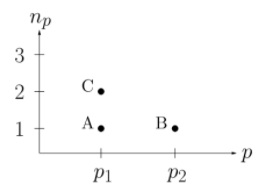
\includegraphics[scale=1]{Figures/occupation.png}
    \caption{A three particle system}
    \label{fig:my_label}
\end{figure}

In this example, we can write the states as $|2100\rangle$. This method is called the occupation number representation.\\
Now looking at the occupation number representation with the Hamiltonian,
\begin{equation}
    \hat{H}|n_1n_2n_3..\rangle=\left[\sum_m n_{p_m}E_{p_m}\right]|n_1n_2n_3...\rangle
\end{equation}
We simply multiply the number of particles in each state by the energy of that state and sum over all of the states.
\subsection{Replacing state vectors with operators}
Next, we are going to remove the state vector representations altogether using the same notation. We use operators to describe the physics rather than state vectors, and we retain only one special state, the vacuum state $|0\rangle$. Taking the harmonic oscillator for example, we can build up a general state of several harmonic oscillators by acting on the vacuum state $|0\rangle$,
\begin{equation}
    |n_1n_2...\rangle=\prod_{k}\frac{1}{(n_k!)}{^1/2}(\hat{a}^\dagger_k)^{n_k}|0\rangle
\end{equation}
Next, we need to verify if these creation and annihilation operators respect the exchange symmetry for identical particles.

\subsection{Indistinguishability and Symmetry}
Putting one particle in state $p_1$ and then another particle in $p_2$, or do the same thing in the reverse order, you should obtain the final state as $|11\rangle$. This means that,
\begin{equation}
    \hat{a}^\dagger_{p_1}\hat{a}^\dagger_{p_2}=\lambda\hat{a}^\dagger_{p_2}\hat{a}^\dagger_{p_1}
\end{equation}
We assume two cases, where $\lambda=\pm 1$, and they correspond to wavefunctions which are either symmetric or antisymmetric under particle exchange.\\
For bosons, $\lambda=1$
\begin{equation}
    \hat{a}^\dagger_{p_1}\hat{a}^\dagger_{p_2}=\hat{a}^\dagger_{p_2}\hat{a}^\dagger_{p_1}
\end{equation}
Rearranging and adding general labels,
\begin{equation}
    [\hat{a}^\dagger_{i}\hat{a}^\dagger_{j}]=[\hat{a}^\dagger_{i}\hat{a}^\dagger_{j}]-[\hat{a}^\dagger_{j}\hat{a}^\dagger_{i}]=0
\end{equation}
which means that the creation operators for different particle states commute. We also have the $[\hat{a}_i,\hat{a}_j]=0$, then,
\begin{equation}
    [\hat{a}_i,\hat{a}^\dagger_j]=\delta_{ij}
\end{equation}
This follows our harmonic oscillator commutation relations, and hence we can build up a state of many particles in momentum states using the formula,
\begin{equation}
     |n_1n_2...\rangle=\prod_{k}\frac{1}{(n_{p_m}!)^}{1/2}(\hat{a}^\dagger_{p_m})^{n{p_m}}|0\rangle
\end{equation}
The commutation of different operators implies that,
\begin{equation}
    \hat{a}^\dagger_{p_1}\hat{a}^\dagger_{p_2}|0\rangle=\hat{a}^\dagger_{p_2}\hat{a}^\dagger_{p_1}|0\rangle=|1_{p_1}1_{p_2}\rangle
\end{equation}
which means that it does not matter which order you put particles in the states, you get the exact same in all cases.\\
Generalising,
\begin{gather}
    \hat{a}^\dagger_i|n_1...n_i...\rangle=\sqrt{n_i+1}|n_1...n_i+1...\rangle\\
    \hat{a}_i|n_1...n_i...\rangle=\sqrt{n_i}|n_1...n_i-1...\rangle
\end{gather}
Now for fermions, we consider $\lambda=-1$, and so,
\begin{equation}
    \{\hat{c}^\dagger_i\hat{c}^\dagger_j\}\equiv \hat{c}^\dagger_i\hat{c}^\dagger_j+\hat{c}^\dagger_j\hat{c}^\dagger_i=0
\end{equation}
We can see that the fermion operators anti-commute, and when we set $i=j$, we find,
\begin{equation}
    \hat{c}^\dagger_i\hat{c}^\dagger_i+\hat{c}^\dagger_i\hat{c}^\dagger_i=0
\end{equation}
Which means that $\hat{c}^\dagger_i\hat{c}^\dagger_i=0$. This means that when we try to put two fermions in the same state, it annihilates it completely. This is the Pauli exclusion principle we saw previously, just with a change in notation. We also get,
\begin{equation}
    \{\hat{c}_i,\hat{c}_j\}=\delta_{ij}
\end{equation}
which means that we can use the harmonic oscillator analogy here as well, but note that order of placing the particle states matters in the case of fermions, because $\hat{c}^\dagger_i\hat{c}^\dagger_j|0\rangle=-\hat{c}^\dagger_j\hat{c}^\dagger_i|0\rangle$
\subsection{The continuum limit}
If we increase the size of the box, the momentum states become more closely spaced until the momentum a continuous variable. The Kronecker $\delta_{ij}$ functions become Dirac $\delta^{(3)}(\textbf{p})$ functions and the sums become integrals,
\begin{equation}
    \hat{a}_{\textbf{p}},\hat{a}^\dagger_{\textbf{q}}=\delta^{(3)}(\textbf{p}-\textbf{q})
\end{equation}
And for energies,
\begin{equation}
    \hat{H}=\int d^3pE_{\textbf{p}}\hat{a}^\dagger_{\textbf{p}}\hat{a}_{\textbf{p}}
\end{equation}
\section{Second Quantization}
\subsection{Field Operators}
Field operators create and annihilate particles in particular momentum states localised at particular spatial locations. Using Fourier sums, we can construct the field operator $\hat{\psi}^\dagger(x)$,
\begin{equation}
    \hat{\psi}^\dagger(x)=\frac{1}{\sqrt{\mathcal{V}}}\sum_{\textbf{p}}\hat{a}^\dagger_{\textbf{p}}e^{-i\textbf{p}\cdot\textbf{x}}
\end{equation}
creates a particle at position $x$, while $\hat{a}^\dagger_{\textbf{p}}$ creates a particle in a state with three-momentum $\textbf{p}$. Similarly the operator $\psi(\textbf{x})$ is defined by,
\begin{equation}
    \hat{\psi}(\textbf{x})=\frac{1}{\sqrt{\mathcal{V}}}\sum_{\textbf{p}}\hat{a}_{\textbf{p}}e^{i\textbf{p}\cdot\textbf{x}}
\end{equation}
annihilates a particle at position $x$, while $\hat{a}_{\textbf{p}}$ annihilates a particle in a state with three momentum $\textbf{p}$.
\subsection{Second quantization of single-particle operators}
We second quantize the n-particle operators by inserting the identities $1=\sum_\alpha=|\alpha\rangle\langle\alpha|$ and $1=\sum_\beta|\beta\rangle\langle\beta|$ into the right hand side of the identity $\hat{\mathcal{A}}=\hat{\mathcal{A}}$,
\begin{equation}
    \hat{\mathcal{A}}=\sum_{\alpha\beta}|\alpha\rangle\langle\alpha|\hat{\mathcal{A}}|\beta\rangle\langle\beta|=\sum_{\alpha\beta}\mathcal{A}_{\alpha\beta}|\alpha\rangle\langle\beta|
\end{equation}
where the matrix element $\mathcal{A}_{\alpha\beta}=\langle\alpha|\hat{\mathcal{A}}|\beta\rangle$.\\
The space that can accommodate multiple particle states is called Fock space, and it is simply defined by,
\begin{equation}
    \mathcal{F}=\bigoplus_{N=0}\mathcal{H}_N=\mathcal{H}_0\oplus \mathcal{H}_1\oplus...
\end{equation}
where $\mathcal{F}$ is the Fock space and the $\mathcal{H}_1$ and $\mathcal{H}_2$, and so on are the single particle Hilbert spaces.\\
The second-quantized version of operator $\hat{\mathcal{A}}$ is simply put as,
\begin{equation}
    \hat{A}=\sum_{\alpha\beta}\mathcal{A}_{\alpha\beta}\hat{a}^\dagger_\alpha\hat{a}_\beta
\end{equation}
What operator $\hat{A}$ essentially does is, it removes a single particle in state $|\beta\rangle$ by using the annihilation operator $\hat{a}_\beta$, multiplies it by the matrix element $\mathcal{A}_{\alpha\beta}$, and then uses $\hat{a}^\dagger_\alpha$ to place the particle into a final state $|\alpha\rangle$.
\subsection{Second quantization of two-particle operators}
The second quantized two particle operator is given by,
\begin{equation}
    \hat{A}=\sum_{\alpha\beta\gamma\delta}\mathcal{A}_{\alpha\beta\gamma\delta}\hat{a}^\dagger_\alpha\hat{a}^\dagger_\beta\hat{a}_\gamma\hat{a}_\delta
\end{equation}
This expression essentially is the sum over all the processes involving the annihilation of two particles in particular states, multiplication by the matrix element, and creation of the two particles in two new states.\\
The two particle operator can also be written in terms of spatial coordinates and field operators as,
\begin{equation}
    \hat{V}=\frac{1}{2}\int d^3xd^3y\hat{\psi}^\dagger(\textbf{x})\hat{\psi}^\dagger(\textbf{y})V(\textbf{x},\textbf{y})\hat{\psi}(\textbf{y})\hat{\psi}(\textbf{x})
\end{equation}
The factor $\frac{1}{2}$ ensures that we do not double count the interactions. We specifically order the operators by placing the creation operators to the left and the annihilation operators to the right, which is known as normal ordering. This makes sure that the operator $\hat{V}$ has zero vacuum expectation value,
\begin{equation}
    \langle 0|\hat{V}|0\rangle=0
\end{equation}
We also order the coordinates, because fermions anticommute, and mixing up the order of the coordinates might result in the wrong operator, but in the case of bosons it really does not matter, since they do commute.


\begin{savequote}[45mm]
Everything in nature is some field configuration.
\qauthor{Urs Schreiber}
\end{savequote}
\chapter{Field Theory}
\section{What is a field?}
 A field is some local function in space with some definite transformations under the symmetries we would like to introduce in the theory. A scalar field is function that spits out a scalar for every point in space=time. Note this scalar can be from $\mathbb{R}$ or $\mathbb{C}$.
\section{Lagrangians for Fields}
When we're talking about fields being elements of the Lagrangian, we need to integrate over all of the field $\phi$
\begin{equation}
    S = \int_{a}^{b} \mathcal{L}(\phi, \partial_{\mu} \phi, t) \ d^{4}x
\end{equation}
We can relate the "new curly" Lagrangian to the old one as follows:
\begin{equation}
   \int_{a}^{b} L dt = \int_{a}^{b} \mathcal{L}(\phi, \partial_{\mu} \phi, t) \ d^{3}x
\end{equation}
We call the new Lagrangian the \textbf{Lagrangian density}. Which also means we can define a momentum density
\begin{equation}
    \Pi = \frac{\partial \mathcal{L}}{\partial(\partial_{\mu} \phi)}
\end{equation}
Now the modified Euler-Lagrange equation reads
\begin{equation}
     \frac{\partial \mathcal{L}}{\partial \phi} - \partial_{\mu} \left( \frac{\partial \mathcal{L}}{\partial(\partial_{\mu} \phi)} \right) = 0
\end{equation}
Similarly we can define the Hamiltonian density as
\begin{equation}
    H = \int_{a}^{b} \ \mathcal{H} \ d^{3}x = \Pi \partial_{\mu} \phi - \mathcal{L}
\end{equation}
Combining all of this we can introduce the of Noether current
\begin{equation}
    j^{\mu} = p^{\mu}\xi - \mathcal{H}^{\mu}_{\rho}\tau^{\rho}
\end{equation}
whose continuity equation reads
\begin{equation}
    \partial_{\mu} j^{\mu} = 0
\end{equation}
\section{The Klein-Gordon Equation}
The Klein-Gordon equation essentially models spin-0 particles without any external potentials i.e. sources.
Let's derive it from what we've seen so far. We start by looking at plane wave solutions to the Schrodinger equation
\begin{equation}
    \phi(x,t) = Ne^{-i(\omega t -k.x)} = Ne^{-ip.x} 
\end{equation}
where $N$ is the normalization constant. We shall call a wave with such a sign combination an \textbf{incoming wave}. So what happens when we operate on it with the energy and momentum operators? We get the following
\begin{equation} \label{energop}
\hat{E}\phi(x,t) = i \hbar \frac{\partial}{\partial t}(Ne^{-i(\omega t -k.x)}) = \hbar \omega \phi(x,t)
\end{equation}

\begin{equation} \label{momenop}
\hat{P}\phi(x,t) = -i \hbar \nabla (Ne^{-i(\omega t -k.x)}) = \hbar k \phi(x,t)
\end{equation}
We have the relation
\begin{equation}
    E = {(p^{2}c^{2} + m^{2}c^{4})}^{1/2}
\end{equation}
Now let's substitute the terms with operators acting on $\phi$
\begin{equation}
    i \hbar \frac{\partial \phi(x,t)}{\partial t} = {(-\hbar^{2}c^{2}\nabla^{2} + m^{2}c^{4})}^{1/2}\phi(x,t)
\end{equation}
This at first glance does not seem covariant, so let's square it
\begin{equation}
    - \hbar^{2} \frac{\partial^{2} \phi(x,t)}{\partial t^{2}} = (-\hbar^{2}c^{2}\nabla^{2} + m^{2}c^{4}) \phi(x,t)
\end{equation}
By setting $\hbar = c = 1$ this can be succintly written as
\begin{equation}
    (\partial^{2} + m^{2}) \phi(x) = 0
\end{equation}
\subsection{Probability Currents}
Although it follows from what we know pretty straightforwardly, it wasn't taken very seriously for one specific reason, let's see why. From the continuity equation we have 
\begin{equation}
    \frac{\partial \rho}{\partial t} = - \nabla . J
\end{equation}
for the case of non-relativistic quantum mechanics, we have
\begin{equation}
    j(x)  = - i\left[ \phi^{*}(x) \nabla \phi - \phi \nabla \phi^{*}(x) \right]
\end{equation}
and for the probability density
\begin{equation}
    \rho(x) = i \left[ \phi^{*}(x) \frac{\partial \phi}{\partial t} - \phi \frac{\partial \phi^{*}(x)}{\partial t} \right]
\end{equation}
these can be combined and written covariantly as
\begin{equation}
    j^{\mu}(x) = i\left[ \phi^{*}(x) \partial_{\mu} \phi - [\partial_{\mu} \phi^{*}(x)]\phi \right]
\end{equation}
Substituting in our wavefunction $\phi(x) = Ne^{-p.x}$, we find that the time component is of the form
\begin{equation}
    j^{0} = \rho = 2{|N|}^{2}E
\end{equation}
Since $E$ can be positive or negative we can't interpret $\rho$ as a probability density as it is non-sensical to talk about negative probabilities. Or is it?
\subsection{A new Interpretation}
Fortunately, not all is lost. Richard Feynman and Ernst Stuckelberg came up with a unique interpretation independently. They suggested that we can view negative energy states as simply particles travelling back in time. What? 
This is because changing the sign of the proper time $\tau$ has the same effect as
changing the sign of the charge. Therefore, a particle travelling backward in time looks the same as an oppositely charged antiparticle moving forward in time. One strategy to eliminate negative energy states
is therefore to reverse the charge and momentum of all negative energy
solutions, turning them into antiparticles. How does this eliminate the
negative sign of the energy? Since we write the phase of the wave function as $Et − p · x$, then making the substitution $t \rightarrow −t$ means that we
have to change $−E \rightarrow E$ for the first term to make sense. Of course
reversing the time (like playing a film backwards) reverses all momenta
so we also need to swap $p \rightarrow −p$ for consistency
We  can visualize this as follows
\begin{figure}
	\centering
	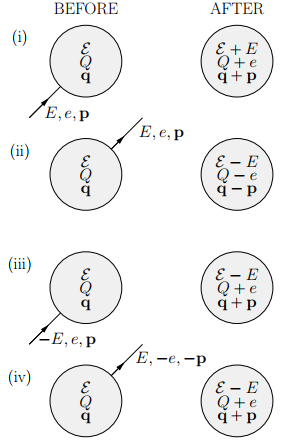
\includegraphics[scale=0.8]{Figures/parvis.png}
	\caption{ (i) An incoming particle (energy $E$, charge $e$ ($= |e|$), momentum
$p$) is absorbed by a system (energy $E$,
charge $Q$, momentum $q$). Also shown
are (ii) emission of particle, (iii) absorption of a particle in a negative energy
state and (iv) emission of an antiparticle in a positive energy state.}
\end{figure}
Thus simply put, a general solution to the Klein-Gordon equation is of the form
\begin{figure}
	\centering
	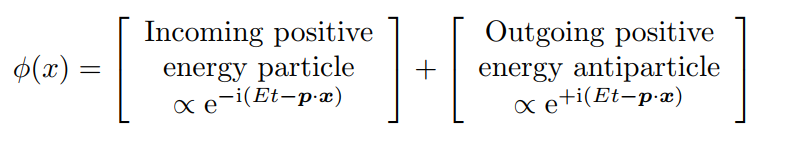
\includegraphics[scale=0.8]{Figures/anti.png}
	\caption{The general solution of the Klei-Gordon equation is a superposition of of positive energy states, only of that of an incoming particle and an outgoing anti-particle}
\end{figure}
We abandon an inherently single-particle description since we have to keep the particles and anti-particles into account.
\section{Field Theories}
A classical field is simply defined as,
\begin{tcolorbox}
A classical field is a piece of mathematical machine that takes a position in spacetime and outputs an object representing the amplitude of the field at that point. The output might be a scalar (in which case we refer to a scalar field), a complex number (a complex scalar field), a vector (in which case we refer to a vector field), a tensor or something more complicated.
\end{tcolorbox}
\subsection{A Massless Scalar Field}
The Lagrangian for a massless salar field $\psi(x)$ is given by,
\begin{equation}
    \mathcal{L}=\frac{1}{2}\partial^\mu\pho\partial_\mu\phi=\frac{1}{2}(\partial_mu\phi)^2
\end{equation}
Where its gradient $\partial_\mu\phi$ is $\partial\phi(x)/\partial x^\mu$. The Lagrangian can also be expanded as,
\begin{equation}
    \mathcal{L}=\frac{1}{2}(\partial_0\phi)^2-\frac{1}{2}\mathbf{\nabla}\phi\cdot\mathbf{\nabla}\phi
\end{equation}
Which neatly resembles $\mathcal{L}=$(kinetic energy)-(potential energy).
\subsection{A Massive Scalar Field}
Including mass in the massless scalar field problem gives us the massive scalar field. In this case, the Lagrangian $\textbf{L}$
also depends on $\phi$, the magnitude of the scalar field along with $\partial_mu\phi$. We do this by introducing a potential energy term $U(\phi)$, and this being proportional to $\phi^2$. Now the Lagrangian can be written as,
\begin{equation}
    \mathcal{L}=\frac{1}{2}(\partial_\mu\phi)^2-\frac{1}{2}m^2\phi^2
\end{equation}
where the $\frac{1}{2}m^2$ factor is to get an interesting result, as we will see below.\\
Using the Lagrangian we obtained, we get the factors,
\begin{equation}
    \frac{\partial L}{\partial\phi}=-m^2\phi
\end{equation}
and,
\begin{equation}
    \frac{\partial L}{\partial(\partial_\mu\phi}=\partial^\mu\phi
\end{equation}
Plugging these into the Euler-Lagrange equation gives us,
\begin{equation}
    (\partial_\mu\partial^\mu+m^2)\phi=0
\end{equation}
We see that the equation of motion of this field theory is the Klein-Gordon equation.
\subsection{An External Source}
Our next step is to introduce interactions into our scalar field. We can do this by introducing a function known as source current $J(x)$, which interacts with the field, giving a potential energy term $-J(x)\phi(x)$. The Lagrangian is written as,
\begin{equation}
    \mathcal{L}=\frac{1}{2}[\partial_\mu\phi(x)]^2-\frac{1}{2}m^2[\phi(x)]^2+J(x)\phi(x)
\end{equation}
And the equations of motion,
\begin{equation}
     (\partial_\mu\partial^\mu+m^2)\phi(x)=J(x)
\end{equation}
\subsection{The $\phi^{4}$ Theory}
To get particles/fields to interact with other particles/fields, we use the $\phi^4$ Lagrangian, where the potential term $U(\phi)$ is proportional to $\phi^4$ instead of $\phi^2$,
\begin{equation}
    \mathcal{L}=\frac{1}{2}\partial^\mu\phi\partial_\mu\phi-\frac{1}{2}m^2\phi^2-\frac{1}{4!}\lambda\phi^4
\end{equation}
which leads to the equation of motion,
\begin{equation}
    (\partial^2+m^2)\phi=-\frac{\lambda}{3!}\phi^3
\end{equation}
Where $\lambda$ is known as the interaction strength. Sadly, this Lagrangian is unsolvable, and we can only use perturbation theory to make predictions out of the $\phi^4$ theory.
\subsection{Two Scalar Fields}
Another method of interacting two particles is by defining two types of particles, described by two fields $\phi_1(x)$ and $\phi_2(x)$. They are said to have the same mass, and interact with themselves and each other via a potential energy $U(\phi_1,\phi_2)=g(\phi^2_1+\phi^2_2)^2$ where $g$ is the interaction strength. The resulting Lagrangian density is given by,
\begin{equation}
    \mathcal{L}=\frac{1}{2}(\partial_\mu\phi_1)^2-\frac{1}{2}(m^2\phi^2_1)+\frac{1}{2}(\partial_\mu\phi_2)^2-\frac{1}{2}(m^2\phi^2_2)-g(\phi^2_1+\phi^2_2)^2
\end{equation}
The above equation shows us the symmetry of the Lagrangian- it does not matter how we define our fields, we still get the same Lagrangian.\\
Transforming the two fields by using the mapping $\phi_1\rightarrow \phi'_1$ and  $\phi_2\rightarrow \phi'_2$, where,
\begin{equation}
    \begin{pmatrix}
    \phi'_1\\
    \phi'_2
    \end{pmatrix}=
    \begin{pmatrix}
    \cos{\theta} & -\sin\theta \\
    \sin\theta & -\cos\theta
    \end{pmatrix}
    \begin{pmatrix}
    \phi_1\\
    \phi_2
    \end{pmatrix}
\end{equation}
then the Lagrangian is still unchanged. We have rotated the fields in $\phi_1-\phi_2$ space. This says that the particles have an internal degree of freedom. The invariance of the physics of the Lagrangian with respect to rotations by $\theta$ in the $\phi_1-\phi_2$ plane expresses an $S0_(2)$ symmetry.
\subsection{The Complex Scalar Field}
A complex field theory can be constructed by making a transformation that simplifies the two scalar fields, by defining two new fields, $\psi$ and $\psi^\dagger$,
\begin{gather}
    \psi=\frac{1}{\sqrt{2}}[\phi_1+i\phi_2]\\
    \psi^\dagger=\frac{1}{\sqrt{2}}[\phi_1-i\phi_2]
\end{gather}
And using the two new fields, we get the Lagrangian,
\begin{equation}
    \mathcal{L}=\partial^\mu\pshi^\dagger\partial_\mu\psi-m^2\psi^\dagger\psi-g(\psi^\dagger\psi)^2
\end{equation}
This is the complex scalar field theory. Although it is made up of two sorts of field, it describes one sort of complex-valued field $\psi$. The Lagrangian is invariant with respect to rotations in the complex plane,
\begin{equation}
    \psi\rightarrow \psi^{i\alpha} \.,\. \psi^{\dagger}\rightarrow e^{-i\alpha}\psi^{\dagger}
\end{equation}
which expresses a $U(1)$ symmetry.
\begin{savequote}[45mm]
Quantization is an art form which, when applied to classical physical theories, yields predictions of subatomic behavior which are in spectacular agreement with experiments. 
\qauthor{Ron Y. Donagi}
\end{savequote}
\chapter{Canonical Quantization}
\section{What is Canonical Quantization}
Canonical Quantization is a tool or a set of mathematical formulations that enables us to transform a classical field into a quantum field by quantizing it. 
In developing canonical quantization we’ll see that particles are added or removed from a system  using field operators and these are formed from the creation and annihilation operators. 
\subsection{How is it done?}
Canonical quantization is done by following a set of processess which enables us to quantize a specific classical field of our choice. They are as follows, 
\begin{enumerate}[I]
    \item Writing down a classical Lagrangian density in terms of fields. This is the most tricky part as there are many possible lagrangians.  
    \item Calculating the momentum density and the Hamiltonian density in terms of fields.
    \item Now consider the fields and momentum density as operators. Pen down the commutation relations on them to make them quantum mechanical.
    \item Expand the fields in terms of creation/annihilation operators.
This will allow us to use occupation numbers and thereby making our job easier. 
  \item Now we have a quantum field considering the fact that we know the normal ordering interpretation. 
\end{enumerate}
\subsection{An Example}
Now lets say we have our Lagrangian for the scalar field at hand. Let's consider the Lagrangian for a massive scalar field given by, 
\begin{equation}
    L = \frac{1}{2} [\delta _{\mu} \phi(x) ]^{2} - \frac{1}{2} m^{2} [\phi(x)]^{2}
 \end{equation}
 The Klein-Gordon equation for this is given by,  $(\delta^{2}+m^{2})\phi = 0$ leading to a dispersion of $E_{p} = p^{2} + m^{2}$. \\
 \\
 Next we find the momentum density, 
 \begin{equation}
     \Pi^{\mu} (x) = \frac{\delta L}{\delta (\delta _{\mu} \phi(x))} 
 \end{equation}
 The time-like component of this tensor is $\Pi^{0}(x)= \pi{x}= \delta^{0} \phi(x)$. This helps us to determine the Hamiltonian in terms of momentum density. 
 \begin{equation}
     H = \Pi^{0}(x)\delta_{0}\phi(x) - L
 \end{equation}
 And now using our Lagrangian, we get the Hamiltonian density, 
 \begin{gather}
     H = \delta^{0} \phi(x) \delta_{0}\phi(x) - L  \\
     = \frac{1}{2} [\delta_{0} \phi(x)]^{2} + [\frac{1}{2} \nabla \phi(x)]^{2} +[\frac{1}{2} m^{2}\phi(x)]^{2}
 \end{gather} 
 We now turn the fields into field operators. We take $\phi(x) -> \hat{\phi}(x)$ and $\Pi^{0}(x) -> \hat{\Pi^{0}}(x)$. To make these field operators quantum mechanical we need to formulate the commutation relations between them. We impose the commutation relation by using the analogous commutation relations that we have in Quantum Mechanics.($[\hat{x}, \hat{p}] = i \hbar $)
 \begin{equation}
     [\hat{\phi}(t,x), \hat{\Pi}^{0}(t,y)] = i \delta ^{(3)} (x,y)
 \end{equation} 
 We also have ,
 \begin{equation}
     [\hat{\phi}(x),\hat{\phi}(y) ] = [\hat{\Pi}^{0}(x), \hat{\Pi}^{0}(y)] = 0 
 \end{equation} 
 This also applies to their dagger versions. \\
 Now the next and the most essential part is where we try to represent all the operators in terms of the annihilation and creation operators. Doing this makes our job very easy and comfortable to work with. \\
 In the case of Coupled oscillators, we have seen that, 
 \begin{equation}
     \hat{x}_{j} = (\frac{h}{m})^{\frac{1}{2}} \sum_{k} \frac{1}{(2 \omega_{k} N )^{\frac{1}{2}}} (\hat{a}_{k}e^{ijka} + \hat{a}^{\dagger}_{k}e^{-ijka}) 
 \end{equation}
 with $E_{p}= (p^{2}+m^{2})$
 In analogy to this, we write down a time-independent field operator for the continuous case as, 
 \begin{equation}
     \hat{\phi}(x) = \int\frac{d^{3}p}{(2\pi)^{\frac{3}{2}}} \frac{1}{(2 E_{p})^{\frac{1}{2}}} (\hat{a}_{p}e^{ip \cdot x} + \hat{a}^{\dagger}_{p}e^{-ip \cdot x})
 \end{equation}
 The commutation relation between the creation and annihilation operators is given by, 
 \begin{equation}
     [\hat{a}_{p}, \hat{a}^{\dagger}_{q}] = \delta^{(3)}(p-q)
 \end{equation}
 To obtain the time dependence on the above equation, we use the Heisenberg interpretation, 
 \begin{equation}
     \hat{\phi}(x) = \hat{\phi}(t,x) = \hat{U}^{\dagger}(t,0) \hat{\phi}(x) {U}^{\dagger}(t,0) = e^{i \hat{H}t} \hat{\phi}(x) e^{-i \hat{H}t}
 \end{equation}
 The creation and annihilation operators act only on $\hat{U}(t,0)$ and hence, 
 \begin{equation}
     \hat{U}^{\dagger}(t,0) a_{p} \hat{U}(t,0) = e^{iE_{p}t} \hat{a}_{p}
 \end{equation}
 This tells us that $\hat{a}_{p}$ picks up at $ e^{-iE_{p}t}$ and $\hat{a}^{\dagger}_{p}$ at $ e^{iE_{p}t}$ \\
 Equation (6.9) is called the mode expansion equation, which we will be covering the upcoming chapters in this section.
 \section{Justifying the Normalizing Factors}
 Now that we've established the mode expansion equation, the unsettling thing that we happen to see is the appearence of random constants in the equation. In this section, let's see how does one arrive at the constants present in that equation. \\
 In the aforementioned integral (equation 6.9),  we see that the momentum term "$d^{3}p$" is not a Lorentz-invariant quantity. We can also use the four momentum representation "$d^{4}p$" where $p= (p^{0}, p)$, but only those values of momenta should be considered for which $p^{2} = m^{2}$. This condition or a constraint is called the \textbf{"Mass shell condition"}
 \begin{figure}[h!]
     \centering
     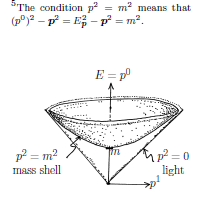
\includegraphics{Figures/massshell.png}
     \caption{Mass Shell}
     \label{fig:my_label}
 \end{figure}
 We write the momentum part as, 
 \begin{equation}
     d^{4}p \: \delta (p^{2}- m^{2}) \theta(p^{0})
 \end{equation}
 Where $\theta(p^{0})$ is called the Heaviside step function. It gives 0 for negative values and 1 for positive values of the function. We use this as we always require the positive values for the above relation. \\
  The Lorentz invariant for this can be written as, 
  \begin{equation}
      \frac{d^{3}p}{(2\pi)^{3}2 E_{p}}
  \end{equation}
  We have included $\frac{1}{(2\pi)}$ for every component of the thee momentum, as the mode expansion is essentially  a reverse fourier transform. \\
  We can normalise the integral by, 
  \begin{equation}
      1= \int \frac{d^{3}p}{(2\pi)^{3}2 E_{p}} \ket{p} \bra{p}
  \end{equation}
  We previously normalized momentum states as $\bra{p}\ket{q}= \delta ^{3}(p-q)$. Hence the four momentum state can be written in terms of the three momentum state as, 
  \begin{equation}
      \ket{p}= (2\pi)^{\frac{3}{2}}(2E_{p})^{\frac{1}{2}} \ket{p}
  \end{equation}
  The new normalization can be written as, 
  \begin{equation}
      \bra{p}\ket{q} = (2\pi)^{3}(2E_{p}) \delta^{(3)} (p-q)
  \end{equation}
  We can define the creation operator $\alpha$ as, 
  \begin{equation}
      \hat{\alpha}^{\dagger}_{p} = (2\pi)^{\frac{3}{2}}(2E_{p})^{\frac{1}{2}} \hat{a}^{\dagger}_{p}
  \end{equation}
  
  Hence our integral becomes, 
  \begin{equation}
       \hat{\phi}(x) = \int\frac{d^{3}p}{(2\pi)^{3}} \frac{1}{(2 E_{p})} (\hat{\alpha}_{p}e^{ip \cdot x} + \hat{\alpha}^{\dagger}_{p}e^{-ip \cdot x})
  \end{equation}
  Now in terms of $\hat{a}^{\dagger}_{p}$ and $ \hat{a}_{p}$, the integral can be rewritten as, 
  \begin{equation}
      \hat{\phi}(x) = \int\frac{d^{3}p}{(2\pi)^{\frac{3}{2}}} \frac{1}{(2 E_{p})^{\frac{1}{2}}} (\hat{a}_{p}e^{ip \cdot x} + \hat{a}^{\dagger}_{p}e^{-ip \cdot x})
  \end{equation}
 \section{What about the Hamiltionian?}
 Now by substituting the expansion of the field operator $\hat{\phi}(x)$ in the hamiltonian equation in terms of the creation and annihilation operators, we get, 
 \begin{equation}
     \hat{H} = \int d^{3}x \frac{1}{2} ([\delta_{0}\phi(x)]^{2} +   [\nabla \phi(x)]^{2} +[ m^{2}\phi(x)]^{2})  
 \end{equation}
 Now we substitute this in the mode expansion equation and use the commutation relations to simplify it. The momentum density calculated is $\hat{\Pi}_{\mu}(x) = \delta _{\mu} \hat{\phi}(x) $ which is given by, 
 \begin{equation}
     \hat{\Pi}_{\mu} = \delta _{\mu} \hat{\phi}(x) =  \int\frac{d^{3}p}{(2\pi)^{\frac{3}{2}}} \frac{1}{(2 E_{p})^{\frac{1}{2}}} (-ip_{\mu}) (\hat{a}_{p}e^{ip \cdot x} + \hat{a}^{\dagger}_{p}e^{-ip \cdot x})
 \end{equation}
 To obtain $\delta _{0} \hat{\phi}(x)$,  we consider only the time-like component of the momentum density. 
 \begin{equation}
     \delta _{0} \hat{\phi}(x) = \int\frac{d^{3}p}{(2\pi)^{\frac{3}{2}}} \frac{1}{(2 E_{p})^{\frac{1}{2}}} (-iE_{p}) (\hat{a}_{p}e^{ip \cdot x} + \hat{a}^{\dagger}_{p}e^{-ip \cdot x})
 \end{equation}
 The space-like components of the momentum density gives us $\nabla \hat{\phi}(x)$, 
 \begin{equation}
     \nabla \hat{\phi}(x) = \int\frac{d^{3}p}{(2\pi)^{\frac{3}{2}}} \frac{1}{(2 E_{p})^{\frac{1}{2}}} (ip) (\hat{a}_{p}e^{ip \cdot x} + \hat{a}^{\dagger}_{p}e^{-ip \cdot x})
 \end{equation}
 Now we have all the necessary factors to compute the hamiltonian. 
 \begin{equation}
     E = \int d^{3} p E_{p} (\hat{a}^{\dagger}_{p}\hat{a}_{p} + \frac{1}{2}\delta^{3}(0))
 \end{equation}
 The last term in the above expression must seem daunting. It leads the above integral to result in infinity. Although we will be working with the difference in the energy levels in which case the term $\frac{1}{2}\delta^{3}(0)$ will cancel out each other. But in terms of the individual expression the equation does not seem to make sense. We need to find a way to device a more reasonable expression in order to get rid of the infinity. The next section will cover the method through which we can deal with this problem.
 
 
 
 
 
 
 
 
 
 
 
 
\section{Normal Ordering}
The infinity that we just encountered is due to the  ambiguity in the Lagrangian. Let's consider a general classical theory formed from complex values fields $\psi(x)$. The Lagrangian describing these fields will contain bilinear terms like $\psi^{\dagger}\psi$ (as we require the Lagrangian to be $\in \mathbb{R}$), which could equally well be written in a classical theory as $\psi\psi^{\dagger}$. However, when we quantize the order that was chosen suddenly becomes crucial. So we undergo a process called \textbf{"Normal ordering"} which removes the ambiguity to give a meaningful quantum theory. We simply need to arrange the operators in a way so that all the creation operators are placed in the left \\
\begin{figure}[!ht]
	\centering
	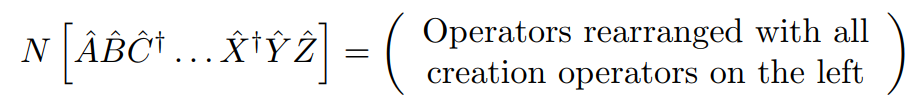
\includegraphics[scale=0.5]{Figures/NormalOrd.png}
	%\caption{A Plot of $\delta(x)$}
\end{figure}
Here $N$ is called the "normal ordering operator", although it doesn't act on states in the traditional sense. When we rearrange operators: there is nothing strange going on for Bose fields, however we do pick up a ${(-1)}^{P}$ (where $P$ is the number of permutations needed to normally order a product of operators) factor when we normally order the product on the left.
Now let's get back to the Hamiltonian, With the normal ordering interpretation the old expression
\begin{equation}
    \hat{H}  = \frac{1}{2} \int d^{3}p \ E_{p}(\hat{a}_{p}\hat{a}^{\dagger}_{p} + \hat{a}^{\dagger}_{p}\hat{a}_{p})
\end{equation}
then becomes
$$N[\hat{H}] = \frac{1}{2} = \int d^{3}p \ E_{p} \ N[\hat{a}_{p}\hat{a}^{\dagger}_{p} + \hat{a}^{\dagger}_{p}\hat{a}_{p}]$$
$$N[\hat{H}] = \frac{1}{2} = \int d^{3}p \ E_{p} \ 2\hat{a}^{\dagger}_{p}\hat{a}_{p}$$
\begin{equation}
     N[\hat{H}] = \int d^{3}p \ E_{p} \ \hat{n}_{p}
\end{equation}
where $\hat{n}_{p} = \hat{a}^{\dagger}_{p}\hat{a}_{p}$ is the number operator. Acting on a state it tells you
how many excitations there are in that state with momentum p.
We now have a Hamiltonian operator that makes sense. 
What we seen now, is that the excited states of the wave equation
can be thought of as particles possessing quantized momenta. These
particles could be called scalar phions after the greek letter Phi ($\phi$) we use to denote the scalar field. They are Bosons with spin $0$. Similarly for spin $1/2$ particles we use spinors and vectors for spin $1$ particles.
\begin{tcolorbox}
\subsection{The Casimir Effect}
Consider two metal plates I and II separated by a distance $L$. We put a third
plate (III) in between them, a distance $x$ from plate I. 
\begin{figure}[!ht]
	\centering
	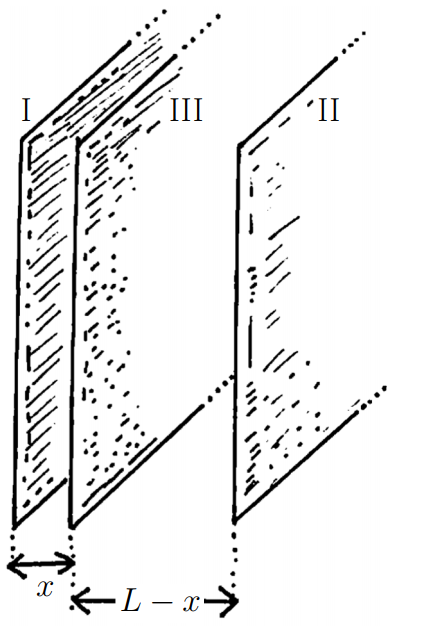
\includegraphics[scale=0.5]{Figures/Casimir.png}
	\caption{A schematic of the Casimir setup}
\end{figure}
We will derive the force on plate III resulting from the field on either side of it. The presence of the plates forces the field to be quantized according to $k_{n} = n \pi/x$ or $n\pi/(L − x)$. The
dispersion is $E_{n} = k_{n}$ and so the total zero-point energy is given by
\begin{equation}
    E = \sum_{n= 1}^{\infty} \left[\frac{1}{2} \left( \frac{n \pi}{x} \right) + \frac{1}{2} \left( \frac{n \pi}{L - x} \right)\right]
\end{equation}
that is, $1/2\hbar \omega_{n}$ per mode as for photons $\omega_{n} = ck_{n}$, and the zero-point energy is $1/2\hbar \omega_{n}$, so in
units in which $\hbar = c = 1$ this becomes
$1/2k_{n}$, and so $E = \sum_{n} 1/2k_{n}$. These sums both diverge, just as we expect since we are evaluating the infinite vacuum energy.
However, real plates can’t reflect radiation of arbitrarily high frequency: the highest energy modes leak out. To take account of this we cut off these high-energy modes
thus:
\begin{equation}
    \frac{n \pi}{2x} \rightarrow \frac{n \pi}{2x}e^{-n \pi a/x}
\end{equation}
We can thus now work out the sums,
$$f(x) = \sum_{n} \frac{n \pi}{2x} e^{-n \pi a/x}$$
$$f(x) = \frac{1}{2} \frac{\partial}{\partial a} \sum_{n}  e^{-n \pi a/x}$$
$$f(x) = \frac{1}{2} \frac{\partial}{\partial a} \frac{1}{1 - e^{n a/x}}$$
\begin{equation}
    f(x) = \frac{\pi}{2x} \frac{\partial}{\partial a} \frac{e^{n a/x}}{{(1 - e^{n a/x})}^{2}} \approxeq \frac{x}{2 \pi a^{2}} - \frac{\pi}{24x} + O(a^{2})
\end{equation}
The total energy between I and II is 
\begin{equation}
    E = f(x) + f(L -x) = \frac{L}{2 \pi a^{2}} - \left(\frac{1}{x} - \frac{1}{L-x}\right) + O(a^{2})
\end{equation}
And if $x << L$, we find a force
\begin{equation}
    F = -\frac{\partial E}{\partial x} = -\frac{\pi}{24 x^{2}}
\end{equation}
which is independent of $a$, as we hoped. Thus, there is an attractive force between
the closely spaced plates I and III. This is the Casimir force. We can understand
this force intuitively by realizing that as the two plates are pulled together we lose
the high-energy modes. This reduces the energy between the plates and leads to
an attractive force. A more quantum-field-theory friendly interpretation is that the
effect results from quantum fluctuations in the vacuum, in which particles are spontaneously created and annihilated
\end{tcolorbox}

\section{Deciphering the Mode Expansion}

However if we recall the Klein-Gordon equation, it had two different solutions. One corresponding to incoming particles and the other to outgoing anti-particles. We can't just
\begin{figure}[!ht]
	\centering
	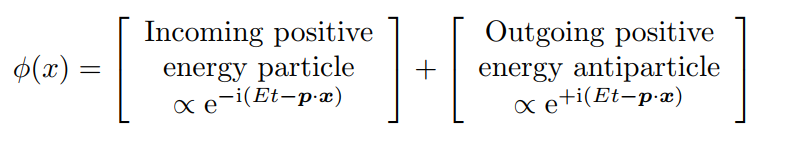
\includegraphics[scale=0.5]{Figures/anti.png}
	\caption{Feynman's interpretation of the solutions to the Klein-Gordon equation}
\end{figure}
The expansion is carried out in terms of incoming plane waves $e^{−ip·x}$.Incorporating Feynman's picture, incoming here means, not only a factor
$e^{−ip·x}$, but also that the particle is annihilated: it comes into the system
and is absorbed by it. Conversely, outgoing means a factor $e^{ip·x}$ and
that the particle is created. We therefore interpret the mode expansion as
\begin{figure}[!ht]
	\centering
	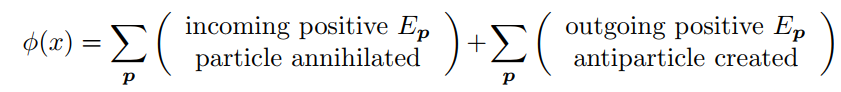
\includegraphics[scale=0.5]{Figures/Parts.png}
	\caption{Interpreting the modified mode expansion}
\end{figure}
The resulting expansion of a field annihilation operator is
\begin{equation}
    \hat{\phi} = \int \frac{d^{3}p}{{(2 \pi)}^{3/2}} \frac{1}{{2 E_{p}}^{1/2}} (\left \hat{a}_{p}e^{-i.px} + \hat{b}^{\dagger}_{p}e^{i.px} \right)
\end{equation}
\section{An Example: Complex Scalar Field Theory}
\subsection{Canonically quantizing the Scalar field}
For complex scalar fields, there are two components, $\psi(x) and (\psi^\dagger(x))$. We need to canonically quantize the Lagrangian using the procedure we saw before.
The Lagrangian for the complex scalar field theory is,
\begin{equation}
    \mathcal{L}=\partial^{\mu}\psi^\dagger(x)\partial_\mu\psi(x)-m^2\psi^\dagger(x)\psi(x)
\end{equation}




\section{The Trouble With Canonical Quantization}
Despite it's outlook, canonical quantization does not work for all theories. It only holds for Lagrangians which cannot be written in terms of quadratic parts composed of it's field and derivatives. The result of canonical quantization is a system described by single particles in momentum states which don’t interact with each other. We refer to the Lagrangians which can be canonically quantized as \textbf{non-interacting theories} and it's opposites as \textbf{interacting theories}. Moreover some have criticized it on being non-fundamental and ad-hoc.

\epigraph{Already from first principles one encounters difficulties. Given that the classical description of a system is an approximation to its quantum description, obtained in a macroscopic limit (when $\hbar \rightarrow 0$), one expects that some information is lost in the limit. So quantization should somehow have to compensate for this. But how can a given quantization procedure select, from amongst the myriad of quantum theories all of which have the same classical limit, the physically correct one?}{\textit{Mac Flecknoe \\ John Dryden}}

\begin{savequote}[45mm]
Gauge symmetry principles are regularly invoked in the context of justification, as deep physical principles, fundamental starting points in thinking about why physical theories are the way they are, so to speak.  
\qauthor{Christopher A. Martin}
\end{savequote}
\chapter{Gauge Theories}
\section{Global Gauge Invariance}

 \begin{figure}[h!]
    \centering
    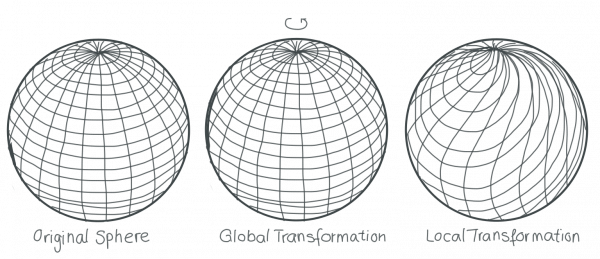
\includegraphics{Figures/localtransformations.png}
    \caption{Gauge Transformations represented pictorially}
    \label{fig:my_label}
\end{figure}

\section{Local Gauge Invariance}

 \begin{figure}
    \centering
    
\includegraphics{Figures/gaugetheornoether.png}
    \caption{Noether's Theorem and Gauge Fields}
    \label{fig:my_label}
\end{figure}

\subsection{Summary}
The Gauge transformation only alters the phase of the field globally
Since the generator of time translations the invariance of the functional implies the invariance of the Lagrangian to the first order in $\epsilon$
\begin{equation}
    \mathcal{L} = \mathcal{L}^{'}
\end{equation}
This gives us the conservation law
\begin{equation}
 \partial_{\mu} j^{\mu} = 0
\end{equation}
where $j^{\mu}$ is defined as
\begin{equation}
    j^{}
\end{equation}
\section{Electrodynamics as a Gauge Theory}

\section{Pure Electrodynamics, Spacetime Invariances and Conservation Laws}
Using the Lagrangian equation for electromagnetic fields, we build the electromagnetic canonical momentum tensor $P_{\rho \sigma}$ of the form, 
\begin{equation}
    P_{\rho \sigma } \equiv \frac {\delta \mathcal{L}}{\delta A^{\rho,\sigma}}
\end{equation}
\begin{equation}
    \frac{\delta (\delta ^{\rho} A^{\sigma})}{\delta (\delta ^{\mu} A^{\nu})} = \delta ^{\rho} _{\mu} \delta^{\sigma}_{\nu}
\end{equation}
Hence we can see that, 
\begin{equation}
    P_{\rho \sigma} = F_{\rho \sigma}
\end{equation}
We can define the Hamiltonian tensor for Pure electromagnetism as, 
\begin{gather}
   \mathcal{H}^{(A) \: \nu}_{\mu} = A^{\rho}_{\mu} P^{\nu}_{\rho}- \delta_{\mu}^{\nu} \mathcal{L}^{(A)} \\
 = (\delta_{\mu} A^{\rho} ) F_{\rho} ^{\nu} - \delta _{\mu}^{\nu} \mathcal{L}^{(A)}
\end{gather}
Now lets look at what happens when an infinitissimal change of $\epsilon$ is made on the spacetime coordinates, 
\begin{gather}
    x^{' \mu} = x^{\mu} + \epsilon  \tau^{\mu} \\
     A ^{' \mu} = A^{\mu} + \epsilon  \tau^{\mu}
\end{gather}
The condition for invariance is , 
\begin{equation}
    \mathcal{L}^{'} G = \mathcal{L} \approx \epsilon^{s}
\end{equation}
When "S>1", it is called as the Jacobian transformation. When this is differentiated with respect to $\epsilon$, and when $\epsilon$ is set to 0, we get the vector field version of fundamental invariance identity of Rund and Trautman, 
\begin{equation}
    -(\frac{\delta \mathcal{L}^{A}}{\delta A^{\mu}} - \delta_{\nu} P_{\mu}^{\nu}) (\mathcal{T}^{\mu} - A^{\mu}_{\sigma} \tau^{\sigma}) = \delta_{\nu}[P_{\rho}^{\nu} \mathcal{T}^{\rho} - \mathcal{H}^{A \: \: \nu}_{\rho} \tau^{\rho} ]
\end{equation}
The LHS becomes zero when it satisfies Euler-Lagrange equation. So if 'j' is invariant under the tranformation shown above, and if 'j' is necessarily an extremal, then equation (7.9) gives the Noether's theorem in the form of the continuity equation, 
\begin{equation}
    S^{\nu} \equiv P_{\rho} ^{\nu} \tau ^{\rho} - \mathcal{H}^{(A)\: \: \nu}_{\rho} \tau ^{\rho}
\end{equation}





\section{Internal Degrees of Freedom}
Internal degrees of freedom are the transformations that we can make between the fields themselves in the Lagrangian. For instance

\section{Non-Abelian Gauge Transformations}
Non-Abelian gauge transformations are simply those which form a non-abelian i.e. non-commutative group.

\subsection{The Kaon Toy Model}


\begin{savequote}[45mm]
Thirty-one years ago, Dick Feynman told me about his ‘‘sum over histories’’ version of quantum mechanics. ‘‘The electron does anything it likes,’’ he said. ‘‘It just goes in any direction at any speed,… however it likes, and then you add up the amplitudes and it gives you the wavefunction.’’ I said to him, ‘‘You’re crazy.’’ But he wasn’t.
\qauthor{Freeman Dyson, 1980t}
\end{savequote}+
\chapter{Concluding Remarks}
Propagators
Functional integral formulation
Next
\chapter*{Appendices}
\setcounter{section}{0}

\addcontentsline{toc}{chapter}{Appendices}
\renewcommand{\thesection}{\Alph{section}}
In this chapter we review all of the necessary mathematics. A knowledge of multivariable calculus and basic probability theory however, is assumed.\section{Mathematical Preliminaries}
\label{appendix_a}
\subsection{Sets}
Let's start with a central concept of belonging. If $x$ belongs to $A$, then we say that $x$ is an element of $A$ i.e. $x$ is contained in $A$, we can the write it as 
\begin{equation}
    x \in A
\end{equation}
\subsubsection{The Axiom of Extension}
\begin{tcolorbox}
    Two sets are equal if and only if they have the same elements
\end{tcolorbox}
Essentially a set, is determined by its extension. Let's say $A$ and $B$ sets, and that every element of $B$ is also an element of $A$, we then call $B$ a subset of $A$, or $A$ inlucdes $B$
\begin{equation}
    B \subset A
\end{equation}
This does not omit the fact that $A \subset A$ holds true despite being trivial, we term this relation to be reflexive i.e. of relating an element to itself. We can then also term equality to be reflexive. However if A and B are sets such that $B \subset A$ and $B \neq A$, the we term $B$ to be a proper subset of $A$. An interesting thing to .think of then is that if $B \subset A$ and $C \subset B$, the we can say that $C \subset A$. This property of a relation is reflexive. Also, inclusion is antisymmetric i.e. $B \subset A \nrightarrow A \subset B$ whereas equality is symmetric i.e. if $A = B$, then necessarily $B =A$.We can then write down the axiom of extension slightly differently
\begin{tcolorbox}
If $A$ and $B$ are sets, then a necessary and sufficient condition for $A = B$ is that both $B \subset A$ and $A \subset B$ hold true
\end{tcolorbox}
It is also interesting to note that belonging and inclusion are conceptually different despite sounding similar: inclusion is always reflexive whereas it is not always clear if belonging is so.
\subsubsection{The Axiom of Specification}
There are two types of "atomic" statements from which the rest can be constructed:
\begin{itemize}
    \item Assertions of belonging: $x \in A$
    \item Assertions of equality: $A = B$
\end{itemize}
We can construct more complicated sentences out of these using logical operators
\begin{center}
\begin{tabularx}{0.99\textwidth} { 
		| >{\raggedright\arraybackslash}X 
		| >{\centering\arraybackslash}X 
		| >{\raggedleft\arraybackslash}X | }
	\hline
\textbf{Operator} & \textbf{Symbol}\\
	\hline
	And & $\wedge$\\
	\hline
	Or (in the sense of either/both)   & $\vee$\\
	\hline
	Not   & $\lnot$ \\
	\hline
	If-then- (or implies) & $\Rightarrow$\\
	\hline
	If and only if (or equivalent to) & $\Leftrightarrow$\\
	\hline
	For some (or there exists) & $\exists$ \\
	\hline
	For all & $\forall$ \\
	\hline
\end{tabularx}
			\end{center}
There are however a few rules to combine them:
\begin{enumerate}[I]
    \item 
    The not comes before a statement which is enclosed in parantheses \footnote{This is done to avoid ambiguity}
    \item And, or and "if and only if" operators are sandwiched between two sentences and the result is enclosed in brackets
    \item 
    \item 
\end{enumerate}
We can now state a major principle of set theory
\begin{tcolorbox}
    \textit{\textbf{Aussonderungsaxiom:}}\textbf{The Axiom of Specification} \\
    For every set $A$ and to every condition/statement $S(x)$ there corresponds a set $B$ whose elements are exactly those elements $x$ of $A$ for which $S(x)$ hold
    \begin{equation}
        B = \left{x \in A: S(x) \right}
    \end{equation}
\end{tcolorbox}
We can illustrate

The moral? To specify a set, it simply not enough to 
\subsubsection{Unordered Pairs}
\subsubsection{Unions and Intersections}
\subsubsection{Complements and Powers}
\subsubsection{Ordered Pairs}
  \subsubsection{Relations}
\subsubsection{Maps}
\subsubsection{Families}
\subsubsection{Inverses and Composites}
\subsubsection{Order}
\subsubsection{Cartesian Product}
Here the symbol "$\times$" means \textbf{"Cartesian Product"} i.e. it's action w.r.t two sets $\mathbb{A}$ and $\mathbb{B}$ is the set of all ordered pairs $(a, b)$ where $a \in \mathbb{A}$ and $b \in \mathbb{B}$

\subsection{Complex Numbers}
\label{appendix_a}
A complex number is an ordered pair $z = \{a,b\} \in \mathbb{C}$ where $a,b \in \mathbb{R}$ where we can denote it as $z = a + ib$ where $i = \sqrt{-1}$
\subsubsection{Addition}
$z_{1} = a_{1} + ib_{1}, \ z_{2} = a_{2} + ib_{2}$
$$z_{1} + z_{2} =  (a_{1} + a_{2}) + i(b_{1} + b_{2})$$
\subsubsection{Multiplication}
$z_{1} = a_{1} + ib_{1}, \ z_{2} = a_{2} + ib_{2}$
$$z_{1}z_{2} =  (a_{1} + ib_{1})(a_{2} + ib_{2}) = (a_{1}a_{2} - b_{1}b_{2}) + i(a_{1}b_{2} + a_{2}b_{1})$$
\subsubsection{Properties}\footnote{$\mathcal{W}, \mathcal{Z}, \lambda \in \mathbb{C}$}
\subsubsubsubsection{Commutativity}
$$\mathcal{W} + \mathcal{Z} = \mathcal{Z} + \mathcal{W}$$
$$\mathcal{W}\mathcal{Z} = \mathcal{Z}\mathcal{W}$$
\subsubsubsubsection{Associativity}
$$(\mathcal{Z}_1 + \mathcal{Z}_2) + \mathcal{Z}_3 = \mathcal{Z}_1 + (\mathcal{Z}_2 + \mathcal{Z}_3)$$
$$(\mathcal{Z}_1\mathcal{Z}_2)\mathcal{Z}_3 = \mathcal{Z}_1(\mathcal{Z}_2\mathcal{Z}_3)$$
\subsubsection{Identities}
$$\mathcal{Z} + 0 = \mathcal{Z}$$
$$\mathcal{Z}1 = \mathcal{Z}$$
\subsubsubsubsection{Additive Inverse}
$$\forall \ \mathcal{Z} \ \exists \ \mathcal{Z}^{-1} \ | \ \mathcal{Z} + \mathcal{Z}^{-1} = 0$$
\subsubsubsubsection{Multiplicative Inverse}
$$\forall \  \mathcal{Z} \neq 0 \ \exists \ \mathcal{W} \ | \ \mathcal{Z}\mathcal{W} = 1$$
\subsubsubsubsection{Distributive Property}
$$\lambda(\mathcal{W} + \mathcal{Z}) = \lambda\mathcal{W} + \lambda\mathcal{Z}$$



\section{Fourier Analysis}
Fourier analysis is the study of a special set of an integral transforms. 
A fourier series is the decomposition of a general wave or oscillation into harmonic components.
Because we treat the wave vector as the independent variable of a wave, the Fourier decomposition
is typically done in terms of wave vectors. A Fourier series is a sum of sinusoidal functions, each of
which is a harmonic of some fundamental wave vector or spatial frequency. A Fourier transform is an
integral over a continuous distribution of sinusoidal functions.
A Fourier series is appropriate when the system has boundary conditions that limit the allowed
wave vectors to a discrete set. For a system where the spatial periodicity is $2L$, the Fourier decomposition of a general periodic function is the series
\begin{equation}
f(x) = \sum_{-\infty}^{\infty} c_{n}e^{i k_{n}x}
\end{equation}
where,
$$k_{n} = \frac{n \pi}{L}$$
Here $c_{n} \in \mathbb{C}$. All $f(x) \in \mathbb{R}$ can be written as:
\begin{equation}
f(x) = \frac{a_{0}}{2} + \sum^{\infty}_{n=1} \left[a_{n}\cos \left(\frac{n \pi x}{L} \right) + b_{n}\sin \left(\frac{n \pi x}{L}\right) \right]
\end{equation}
Where,
\begin{equation}
	a_{n} = \frac{1}{L} \int_{0}^{2L} f(x) \cos\left(\frac{n \pi x}{L}\right) dx
\end{equation}
\begin{equation}
	b_{n} = \frac{1}{L} \int_{0}^{2L} f(x) \sin\left(\frac{n \pi x}{L}\right) dx
\end{equation}
\begin{equation}
	c_{n} = \frac{1}{2L} \int_{0}^{2L} f(x) e^{-ik_{n}x}dx
\end{equation}
obtained by calculating the overlap integrals (i.e., projections or inner products) of the desired function with the harmonic basis functions. That is provided $f(x)$, obeys the following conditions i.e. \textbf{Dirichlet conditions}:
\begin{itemize}
\item It must be absolutely integrable over a period.
\item It must be of bounded variation in any given bounded interval.
\item It must have a finite number of discontinuities in any given bounded interval, and the discontinuities cannot be infinite.
\end{itemize}
A Fourier transform is appropriate when the system has no boundary conditions that limit the allowed wave vectors. In this case, the Fourier decomposition is an integral over a continuum of wave vectors:
\begin{equation}
	f(x) = \frac{1}{\sqrt{2 \pi}} \int_{-\infty}^{\infty} a(k)e^{ikx}dk
\end{equation}
where  the  expansion  function  $a(k)$  is  complex. To  obtain  the  expansion  function  $a(k)$  for  a  givenspatial function $f(x)$ requires the inverse Fourier transform
\begin{equation}
	a(k) = \frac{1}{\sqrt{2 \pi}} \int_{-\infty}^{\infty} f(x)e^{-ikx}dx
\end{equation}
which is a projection of the spatial function $f(x)$ onto the harmonic basis functions $e^{ikx}/\sqrt{2 \pi}$. The basis functions are orthogonal and normalized in the Dirac sense, which means their projections onto each other are Dirac delta functions
\begin{equation}
\begin{split}
	\frac{1}{2 \pi} & \int_{-\infty}^{\infty} e^{ik^{'}x}e^{-ikx}dx = \delta(k-k^{'})\\
	\frac{1}{2 \pi} & \int_{-\infty}^{\infty} e^{ikx^{'}}e^{-ikx}dk = \delta(x-x^{'})
\end{split}
\end{equation}
\subsection{Parseval’s theorem}
Parseval’s theorem states that the power is the same whether calculated in position space or wave-vector space:
\begin{equation}
\int^{\infty}_{-\infty} \abs{f(x)}^{2}dx = \int^{\infty}_{-\infty} \abs{a(k)}^{2}dk
\end{equation}

\section{The Dirac Delta Function}
\subsection{The Divergence of $\frac{\hat{r}}{r^{2}}$}
We can see why the divergence is,
\begin{equation}
\nabla . \frac{\hat{r}}{r^{2}} = 0
\end{equation}
But if we calculate this using the Divergence theorem, we find that ,
\begin{equation}
	\oint v .da = \int \left( \frac{\hat{r}}{r^{2}} \right) . \left( r^{2} \sin(\theta) d \theta d \phi \hat{r} \right) = \left( \int_{0}^{\pi} \sin(\theta) d \theta \right) \left( \int_{0}^{2\pi} d \phi \right) = 4 \pi
\end{equation}
This is paradoxical. The issue is that it blows up at $r=0$ but is is neglible everywhere else. How do we fix this? The Dirac Delta functional!
\subsection{The One-Dimensional Dirac Delta Functional}
The Dirac Delta is a functional \footnote{An object that is a map between functions} which we define as,
\begin{equation} \label{deltadef}
\delta(x-a)= 
\begin{cases}
0, & \text{if } x \neq a\\
\infty,              & \text{if } x = a
\end{cases}
\end{equation}
\begin{equation}
\int_{- \infty}^{+ \infty} \delta(x-a) dx = 1
\label{del2}
\end{equation}
$\forall \  a \in \mathbb{R}$
We can visualize it as a sharp peak at $a$,
\begin{figure}[!ht]
	\centering
	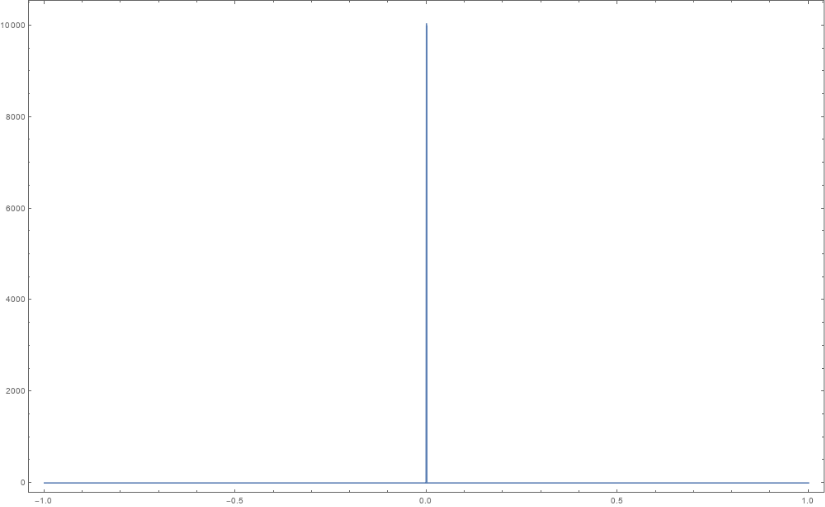
\includegraphics[scale=0.5]{Figures/delta-distribution.png}
	\caption{A Plot of $\delta(x)$}
\end{figure}
We can interpret \ref{del2} as saying "the area of the delta distribution is always 1".
\begin{equation}
f(x)\delta(x - a ) = f(a)
\end{equation}
We can combine these to get,
\begin{equation}
\int_{- \infty}^{+ \infty} \delta(x-a) f(x) dx = f(a)
\end{equation}
\subsubsection{A few interesting properties}
\begin{equation}
\delta(kx) = \frac{1}{|k|}\delta(x)
\end{equation}
\begin{equation}
\frac{d}{dx}(\delta(x)) = -\delta(x)
\end{equation}
where k is a constant
\begin{equation}
\frac{d \theta}{dx} = \delta(x)
\end{equation}
Where $\theta$ is the step function defined as,
\begin{equation}
\theta(x)= 
\begin{cases}
1, & \text{if } x > 0\\
o,              & \text{if } x \leq 0
\end{cases}
\end{equation}

\subsection{The Three-Dimensional Dirac Delta Function}
We generalize (\ref{deltadef}) to three dimensions,
\begin{equation}
\delta^{3}(\vec{r} - \vec{a}) = \delta(x-a_{x})\delta(y-a_{y})\delta(z-a_{z})
\end{equation}
\begin{equation}
\int_{- \infty}^{+ \infty} \delta^{3}(\vec{r} - \vec{a}) dV = 1
\end{equation}
We can also define the three-dimensional delta function as
\begin{equation}
\delta^{3}(\boldscriptr) = \frac{1}{4 \pi} \left[\nabla \cdot \left( \frac{\hat{\boldscriptr}}{{\scriptr	}^{2}}\right)\right]
\end{equation}
Since,
$$\nabla \left(\frac{1}{\scriptr}\right) = -\frac{\hat{\boldscriptr}}{\scriptr^{2}}$$
We can rewrite as,
\begin{equation}
\delta^{3}(\boldscriptr) = -\frac{1}{4 \pi} \left[\nabla^{2}  \left( \frac{1}{\scriptr}\right)\right]
\end{equation}
\subsection{Integral representation}
We have the relationship for the Fourrier transform,
\begin{equation}
F(x) = \int f(t) e^{-ixt} dt
\end{equation}
and it's inverese
\begin{equation}
f(t) = \frac{1}{2 \pi} \int F(x) e^{ixt} dx
\end{equation}
Plugging in Eq. into Eq. we find that 
\begin{equation}
	F(y) = \frac{1}{2 \pi} \int_{-\infty}^{\infty} F(x) dx \int_{-\infty}^{\infty}e^{i(x-y)t} dt
\end{equation}	
Now, invoking the definig property of the Delta function,
\begin{equation}
F(y) = \int_{-\infty}^{\infty} F(x) \delta(x-y) dx
\end{equation}
Comparing and we find that,
\begin{tcolorbox}
\begin{equation}
\delta(x-y) = \frac{1}{2 \pi} \int_{-\infty}^{\infty} e^{i(x-y)t} dt
\end{equation}
\end{tcolorbox}

\section{ Algebra}
\label{ap:algebra}
\subsection{Fields}
A field is a set along with two operations which follow a bunch of axioms/rules. But for our case, we can simply assume that a field $\mathcal{F}$ is either $\mathbb{R}$ or $\mathbb{C}$
\subsection{Vector Spaces}
A linear vector space or simply a vector space $\mathbb{V}$ is a set along with the multiplication $(.)$ and addition $(+)$ operations over a field $\mathcal{F}$, such that the following axioms hold\footnote{Here, $\alpha , \beta \in \mathcal{F}$ and $\ket{u}, \ket{v} $ and $\ket{w} \in \mathbb{V}$}:
\begin{itemize}
	\item \textbf{Commutativity:} $\ket{u} + \ket{v} = \ket{v} + \ket{u}$
	\item \textbf{Associativity:} $(\ket{u} + \ket{v}) + \ket{w} = \ket{v} + (\ket{u} + \ket{w})$
	\item \textbf{Additive Identity:} 
	$\exists \  \ket{0} \in \mathbb{V} \ | \ \ket{v} + \ket{0} = \ket{0} + \ket{v} = \ket{v}$
	\item \textbf{Additive Inverse:} $\forall \ \ket{v} \ \exists \ \ket{v^{-1}} \ | \ \ket{v} + \ket{v^{-1}} = 0$
	\item \textbf{Multiplicative identity:} $\exists \ 1 \in \mathbb{V} \ | \ 1 .\ket{v} = \ket{v}$
	\item \textbf{Multiplicative Associativity:}  $(\alpha \beta) \ket{v} = \alpha (\beta \ket{v})$
	\item \textbf{Distributive Properties:} 
	\begin{itemize}
		\item $(\alpha + \beta) \ket{u} = \alpha \ket{u} + \beta \ket{u}$
		\item $\alpha (\ket{u} + \ket{v}) = \alpha \ket{u} + \alpha \ket{v}$
	\end{itemize}
\end{itemize}
Some examples of vector spaces:
\begin{itemize}
    \item The set of all $n \times n$ invertible matrices with complex entries: $M_{n}(\mathbb{C})$
    \item The set of all $n \times n$ Hermitian i.e. $A = A^{\dagger} = {(A^{T})}^{*}$ matrices with complex entries: $H_{n}(\mathbb{C})$
    \item The set of all square-integrable complex-valued functions on an internval $[a,b]$: $L^{2}([a,b])$
\end{itemize}

\subsection{Subspaces}
Given a vector space $\mathbb{V}$, a subset of its elements that form a vector space among themselves is called a subspace. We will denote a particular subspace $i$ of dimensionality $n_{i}$ by $\mathbb{V}^{n_{i}}_{i}$.\\
   Given two subspaces, and , we define their sum $\mathbb{V}^{n_{i}}_{i} \oplus \mathbb{V}^{m_{i}}_{i} = \mathbb{V}^{l_{i}}_{i}$ as the set containing:
\begin{enumerate}
\item All the elements of $\mathbb{V}^{n_{i}}_{i}$
\item All the elements of $\mathbb{V}^{m_{j}}_{j}$
\item And all possible linear combinations of the above
\end{enumerate} 
However for the elements of (3), closure is lost. The dimensionality of such a subspace is $n + m$.
\subsection{Bases, Span and Linear Independence}
\begin{itemize}
    \item If $S = \{\ket{v}_{1},\ket{v}_{1},...,\ket{v}_{k}\} \subset \mathbb{V}$ is a set of $k$ vectors in $\mathbb{V}$, then the span of $S$, denoted $Span \{\ket{v}_{1},\ket{v}_{2},...,\ket{v}_{k} \}$ or Span S, is defined to be just the set of all vectors of the form $\{c^{1}\ket{v}_{1} + c^{2}\ket{v}_{2} + .... + c^{k}\ket{v}_{k} \}$
    \item Such vectors are known as linear combinations of the $v_i$, so Span $S$ is just the set of all linear combinations of the vectors in $S$
    \item A basis for a vector space $\mathbb{V}$ is a linearly independent set $\mathcal{B} \subset \mathbb{V}$ whose span is all of $\mathbb{V}$
    \item The dimension of a vector space $\mathbb{V}$, denoted $dim \ \mathbb{V}$ , is the number of
elements of any finite basis
\item If no finite basis exists, then we say that $\mathbb{V}$ is infinite dimensional.
\item Components are simply the scalar coefficients with respect to a specific basis
\item Vectors exist independently of any chosen basis
\item Vectors transform (contravairant) in the opposite way (the inverse of the original transformation matrix) to which it's basis transforms (covariant)
\end{itemize}

\subsection{Linear Maps}
A linear map/transformation is simply transformation $\hat{L}$ that
		\begin{itemize}
				\item Adds inputs or outputs, $\hat{L}(\ket{v} + \ket{w}) = \hat{L}(\ket{v}) + \hat{L}(\ket{w})$
			\item Scale the inputs or outputs, $\hat{L}(\alpha \ket{v}) = \alpha \hat{L}(\ket{v})$
		\end{itemize}
		Here, $\alpha  \in \mathcal{F}$ and $\ket{v} $ and $\ket{w} \in \mathbb{V}$
\subsection{Hermitian Forms}
Every vector space $\mathbb{V}$ has a dual space $\mathbb{V}^{*}$
\begin{itemize}
\item $\forall \ \ket{v} \ \exists \ \bra{w} := \ket{v} \rightarrow \mathbb{R}$
\item Much like a vector space, one can assign the dual space a Basis set $e^{i}$
\item It is common to set the basis up in a way that $$e^{i}(e_{j}) = \delta^{i}_{j} = \begin{cases}            1, &         \text{if } i=j,\\
            0, &         \text{if } i\neq j.
    \end{cases}$$
\end{itemize}
A non-degenerate Hermitian form on a vector space $\mathbb{V}$ is a function
$\langle \cdot | \cdot \rangle$ which assigns to an ordered pair of vectors $\ket{v}, \ket{w} \in \mathbb{V}$ a scalar, denoted $\braket{v}{w}$,
having the following properties:
\begin{itemize}
    \item \textbf{Linearity for the vectors:} $\bra{U}(\alpha\ket{V}+\beta\ket{W}) = \bra{U}\alpha\ket{V} + \bra{U}\beta\ket{W} = \alpha\braket{U}{V} + \beta\braket{V}{W}$
    \item \textbf{Hermicity/Skew-symmetry:} $\braket{V}{W} = {(\braket{W}{V})}^{*}$
    \item \textbf{Non-degeneracy:} For each $\ket{v} \neq 0 \in \mathbb{V}$, there exists $w \in \mathbb{V}$ such that $\braket{v}{w} \neq 0$
    \item \textbf{Positive-Definiteness:} $\braket{V}{V} > 0$, for all $\ket{V} \neq \ket{0}$
\end{itemize}
\begin{itemize}
    \item There exists a symmetric bilinear function $g$ that maps Vectors to Duals i.e. $g : = \ket{v} \rightarrow \bra{v}$
    \item $\bra{v}$ is termed the metric dual
\end{itemize}

\subsection{Kernels}
For any linear map $\hat{T}$, a Kernel is a set of all vectors whose image is the zero vector. We often denote this space as $Ker(\hat{T})$.

%\subsection{Inner Product}
%A (sesquilinear i.e. half-linear) inner product is a generalization of the dot product that we are familiar with. It is defined as follows, the operation $\langle . | . \rangle$
%\begin{itemize}
 %   \item \textbf{Skew-symmetry:} $\langle V | W \rangle = { \langle W | V \rangle}^{*}$
  %  \item \textbf{Positive semidefiniteness:} $\langle V | V \rangle \geq 0$,* unless and until *$| V \rangle = | 0 \rangle$
   % \item \textbf{Linearity for the vectors:} $\langle U | (\alpha | V \rangle+\beta | W \rangle) = \langle U | \alpha | V \rangle + \langle U | \beta | W \rangle = \alpha \langle U |  V \rangle+ \beta \langle V |  W \rangle$*
%\end{itemize}
%Where, $\alpha \in \mathbb{C}$ and $| U \rangle,| V \rangle,| W \rangle \in \mathbb{V}$ and $\langle U| ,\langle V |, \langle W| \in \mathbb{V}^{*}$

\subsection{Hilbert Spaces}
A Hilbert space is an inner product vector space $\mathcal{H}$ that
\begin{itemize}
    \item has an norm i.e. length defined as $||V|| =  \sqrt{\langle V | V\rangle}$
    \item  is complete i.e. all of it's Cauchy sequences converge
\end{itemize}
A Cauchy sequence is simply a sequence of numbers whose succeeding term is smaller than the preceding one and when taken to a limit it converges. That is if you have a sequence One can visualize this as the plot of a dampened oscillator.

\subsection{Tensors}
A tensor is defined as a multilinear (i.e. linear in every argument) map $T(r,s)$ of the form
\begin{equation}
    \underbrace{V \times V \times V \times ...}_\text{r-times} \times \underbrace{V^{*} \time V^{*} \time V^{*} \times ...}_\text{s-times} \rightarrow \mathbb{R}
\end{equation}
\subsection{The Tensor Product}
A tensor product operation of two vectors $V \otimes W$ is defined as a bilinear function that maps $V^{*} \times W^{*}$ to the underlying field whose action is defined as
\begin{equation}
    (v \otimes w)(h,g) = v(h)w(g) \ \forall \ h \in V^{*}, g \in W^{*}
\end{equation}
Often times, a tensor is simply the set of all coefficients put in a matrix for such a map.
\subsection{A few interesting tensors}
\subsubsection{Kronecker delta}
It simply has the ‘function’ of ‘renaming’ an index:
$$\delta^{\mu}_{\nu} x^{\nu} = x^{\mu}$$
it is in a sense simply the identity matrix.
\subsubsection{Levi-Civita Pseudotensor}
\label{Levi}
The Levi-Civita Pseudotensor i.e. Tensor density is a completely anti-symmetric i.e. $\epsilon_{ijk} = -\epsilon_{jik} = -\epsilon_{ikj} = -\epsilon_{kji}$, we define it as:
\begin{equation}
\epsilon_{ijk} = \begin{cases}
1 \ \text{if } ijk \text{ is an even permuation of } 123\\
-1 \ \text{if } ijk \text{ is an odd permuation of } 123\\
0  \text{ if two indices are equal}\\
\end{cases}
\end{equation}
We have the identity
\begin{equation}
\epsilon_{\alpha \beta \nu}\epsilon_{\alpha \beta \sigma} = \delta_{\mu \rho} \delta_{\nu \sigma} - \delta_{\mu \sigma}\delta_{\nu \rho}
\end{equation}
From this it follows that,
\begin{equation}
\epsilon_{\alpha \beta \nu}\epsilon_{\alpha \beta \sigma} = 2\delta_{\nu \sigma}
\end{equation}
and
\begin{equation}
\epsilon_{\alpha \beta \gamma}\epsilon_{\alpha \beta \gamma} = 6
\end{equation}
Using these identities and the definition we can rewrite the cross-product of two vectors as,
\begin{equation}
\vec{a} = \vec{a} \cross \vec{b}  = \epsilon_{ijk}a_{j}b_{k}
\end{equation}
Thus the expressions in vector product notation can be changed to index notation for example,
$$
c = \nabla.(\nabla \cross \vec{a}) = \nabla_{i}(\epsilon_{ijk}\nabla_{j}a_{k}) = \epsilon_{ijk}\partial_{i}\partial_{j}a_{k}
$$
because,
$$\nabla_{i} = \frac{\partial}{\partial x_{i}} := \partial_{i}$$


\section{Complex Analysis}
\label{appendix_c}
\subsection{Analytic Functions}
A complex valued function, 
\begin{equation}
    f(z) = u(x,y) + iv(x,y)
\end{equation}
for $z = x + iy$ is said to be analytic in a region close to a point $z$, then it has a derivative at every point in that region i.e. neighbourhood. We define it's derivative as:
\begin{equation}
   f^{'}(z)  = \frac{df}{dz} = \lim_{\delta z  \rightarrow 0}\frac{\delta f(z + \delta z) - f(z)}{\delta z}
\end{equation}
An important point here is that $f^{'}(z)$ should not depend on the way $\delta z$ is selected. An alternate way to state this is to mandate that the Cauchy-Riemann relations,
\begin{equation}
    \begin{aligned}
    \frac{\partial u}{\partial x} = \frac{\partial v}{\partial y} \\
    \frac{\partial v}{\partial x} = - \frac{\partial u}{\partial y}
    \end{aligned}
\end{equation}
hold for $f(z)$.
\subsection{Poles}
A pole is a type of singularity i.e. a point where a mathematical object is not defined
. Think of the function $1/ z^{n}$ at $z = 0$. Let's suppose a function $f(z)$ is analytic between $C_{1}$ and $C_{2}$. In the region between them we can expand out $f(z)$ about a point $z_{0}$ as a Laurent series
\begin{equation}
    f(z) = a_{0} + a_{1} {(z- z_{0})} + a_{2} {(z- z_{0})}^{2} + ... + \frac{b_{1}}{{(z- z_{0})}} + \frac{b_{1}}{{(z- z_{0})}^{2}} + ...
\end{equation}
The part of the series with the b coefficients is termed as the principal part of the series. From this we can draw a few conclusions:
\begin{itemize}
    \item If all $b_{i}$'s are zero then $f(z_{0})$ is analytical at $z = z_{0}$
    \item If all $b_{i}$'s (termed the residue of $f(z)$ at $z = z_i$) after $b_{n}$ are zero then we can say that we have a pole of order $n$ at $z = z_0$ (if $n = 1$, then we say we have a simple pole)
    
\end{itemize}
\subsection{Contour Integrals}
A contour $C$ is a closed path in $\mathbb{C}$ with a finite number of corners that doesn't cross itself. We will now review interesting things about integrals around such contours as, often we want to do difficult integrals over real variables. These may
be turned into easier integrals if we form a contour in the complex plane
which includes the original domain of integration which turn out to be much more tractable. The art is in choosing the best contour to do the integral
\subsubsection{Cauchy's Theorem}
If $f(z)$ is analytic on and inside $C$, then
\begin{equation}
    \oint_{C} dz \ f(z) = 0
\end{equation}
\subsubsection{Cauchy's Integral Formula}
If $f(z)$ is analytic on and inside a simple closed curve $C$ and a point a inside the curve, then 
\begin{equation}
    f(a) = \frac{1}{2 \pi i} \oint_{C} dz \frac{f(z)}{z-a}
\end{equation}
\subsubsection{Residue Theorem}
If $f(z)$ has singularities at points $z_{i}$, then for a contour $C$ that encloses them we have
\begin{equation}
    \oint_{C}dz \ f(z) = 2 \pi i \sum_{i} \text{Residue} \ \text{at} \ f(z_{i}) \ \text{inside} \ C
\end{equation}
wherein the integral is evaluated anti-clockwise i.e. we do it clockwise and simply invert the sign
\subsection{Branch Cuts}
Due to the multivaluedness of functions in $\mathbb{C}$, we need to set "limits" to where our contours can be drawn and where they cannot. A \textbf{branch cut} along a curve essentially states that the analytic function is discontinuous along it/we aren't interested in that region and thus implies that a contour cannot be taken along that path.
\begin{figure}
	\centering
	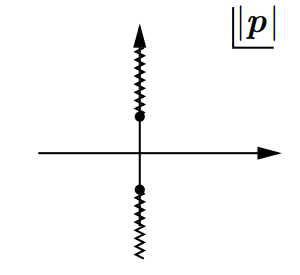
\includegraphics[scale=0.5]{Figures/branc.png}
	\caption{The branch cuts for the integral $\frac{-i}{{(2 \pi)}^{2}|x|}\int_{-\infty}^{\infty}d|p||p|e^{i|p||x|}.e^{-it\sqrt{{|p|}^{2}+{m}^{2}}}$}
\end{figure}
We term the points where the function is multivalued as branch points. Note: the starting/ending points of branch cuts needn't be branch points.

\subsection{Cauchy's Principal Value Method}
For an integral
\begin{equation}
    \int^{c}_{a} dz \ f(z)
\end{equation}
Let us suppose there exists a pole at b where $a < b < c$. How would we evaluate this? This is where we take the "principal value" $\mathcal{P}$ of the integral
\begin{equation}
    \mathcal{P} \int^{c}_{a} dz \ f(z) = \lim_{\epsilon \rightarrow 0^{+}} \left[  \int^{b- \epsilon}_{a} dz \ f(z) + \int^{c}_{b + \epsilon} dz \ f(z) \right]
\end{equation}
to obtain an unambiguous value. When we consider integrals of the form
\begin{equation}
    \int^{b}_{a} dz \ \frac{f(z)}{z + i \epsilon}
\end{equation}
where $f(z): \mathbb{C} \rightarrow \mathbb{C}$ and $a < 0 < b \in \mathbb{R}$, we use the identity
\begin{equation}
    \lim_{\epsilon \rightarrow 0^{+}} \int^{b}_{a} dz \ \frac{f(z)}{z \pm i \epsilon}  = \mathcal{P} \int^{b}_{a} dz \ \frac{f(z)}{z} \mp f(0)
\end{equation}
We then take $f(z - z_{0}) = \delta (z - z_{0})$ to obtain
\begin{equation}
    \frac{1}{z_{0} \pm i \epsilon} = \frac{\mathcal{P}}{z_{0}} \mp i \pi \delta(z_{0})
\end{equation}
\section{Group Theory}
\label{appendix_d}
\subsection{Preliminaries}
\subsubsection{Definition of a Group}
A Group is an algebraic structure i.e. a set with an operation $(G, \circ)$ which follows the axioms:
\begin{itemize}
    \item The operation is well-defined: $\forall \ a,b,c,d \in G \text{ if } a = d: a \circ b = c \implies d \circ b = c$
    \item Closure: $\forall \ a,b \in G: a \circ b \in G$
    \item Associativity: $\forall \ a,b,c \in G: a \circ (b \circ c) = (a \circ b) \circ c$	
    \item Existence of a unique Identity: $\exists \ e \in G : \forall \ a \in G: a \circ e = e \circ a =
    a$	
    \item Existence of an unique Inverse for each element: $\forall \ a \in G: \exists \  a^{-1} \in G: a \circ a^{-1} = a^{-1} \circ a = e$	
\end{itemize}
A group which displays commutativity is termed abelian and it's oppsite is called non-abelian.
\begin{figure}
	\centering
	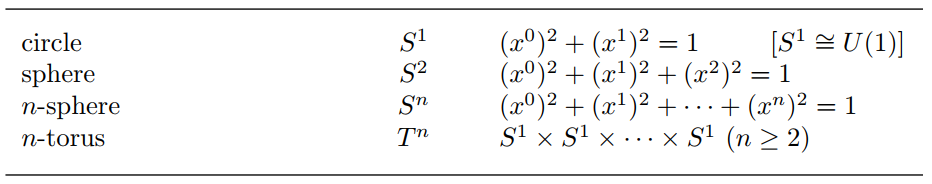
\includegraphics[scale=0.5]{Figures/Groups.png}
	\caption{Some examples of groups}
\end{figure}

\subsubsection{Subgroup}
For a group $(G, *)$, a subgroup $H \subseteq G$ is defined as a group with the same composition binary operator. The notation $H \leq G$ is often used to indicate that $H$ is a subgroup of $G$

\subsubsection{Cosets}
If $G$ is a group and $H \leq G$, then $\forall g \in G, h \in H$:
\begin{itemize}
    \item The set $g*H = {g*h}$ is termed the left coset of $H$ in $G$
    \item The set $H*g = {h*g}$ is termed the left coset of $H$ in $G$
\end{itemize}
\subsubsection{Normal Subgroup}
A subgroup $N \leq G$ whose left and right cosets are equal is termed a \textbf{normal subgroup}, denoted by $N \trianglelefteq G $
\subsubsection{Quotient Group}
For a group $G$ and a normal subgroup $N$ of $G$, the \textbf{quotient group} of $N$ in $G$, written $G/N$ and read "$G$ modulo $N$", is the set of cosets of $N$ in $G$.

\subsubsection{Morphisms}
A \textbf{group homomorphism} $\phi : G \rightarrow H$ is a map between two groups $G(G, *)$ and $H(H, +)$ that preserves the group structure i.e.
\begin{equation}
    \phi(a * b) = \phi(a) + \phi(b) \ \forall \  a,b \in G
\end{equation}
This preserves the group structure because:
\begin{itemize}
    \item This maps identity elements to identity elements i.e. $\phi(e_G) = e_{H}$
    \item $\phi(g^{-1}) = {\phi(g)}^{-1}$
\end{itemize}
The \textbf{Kernel} of a group homorphism $\phi : G \rightarrow H$ is the set of all elements of $G$ that are sent to the identity of $H$ i.e. $ker\phi = \{ g \in G | \phi(g) = e_{G}\}$
\begin{tcolorbox}
\textbf{Proposition:} A group homomorphism $\phi: G \rightarrow H$ is injective if and only if it's Kernel is trivial i.e. $ker\phi = \{ e_{G} \}$
\end{tcolorbox}
Two groups $G$ and $H$ are said to be \textbf{isomorphic} i.e. $G \cong H$ if there exists an invertible group homomorphism $\phi : G \rightarrow H$ i.e. an \textbf{isomorphism}
\begin{tcolorbox}
    \textbf{Isomorphism Theorem}\\
    Let $\phi: G \righarrow H$ be a group homomorphism. Then:
    \begin{itemize}
        \item $Im(\phi) \leq H$
        \item $Ker(\phi) \trianglelefteq G$
        \item $Im(\phi) \cong G/Ker(\phi)$
    \end{itemize}
\end{tcolorbox}
\subsection{Lie Groups}
A matrix Lie group is essentially a closed \footnote{Closed w.r.t to a topology induced from $M_{n}(\mathbb{C})$} using the operator norm\footnote{$||A|| = sup \{ \frac{||A||}{||X||} | \ X \in \mathbb{C}^{n} \textbackslash \{0\} \}$} subgroup of the general linear group\footnote{$GL(n, \mathbb{C}) = \{ A \in M_{n}(\mathbb{C}) \ | \ det(A) \neq 0\}$ i.e. the set of all linear transformations on a vector space over $\mathbb{C}$ } $G \leq GL(n, \mathbb{C})$ for some $n \in \mathbb{N}$ where, 
\begin{figure}
	\centering
	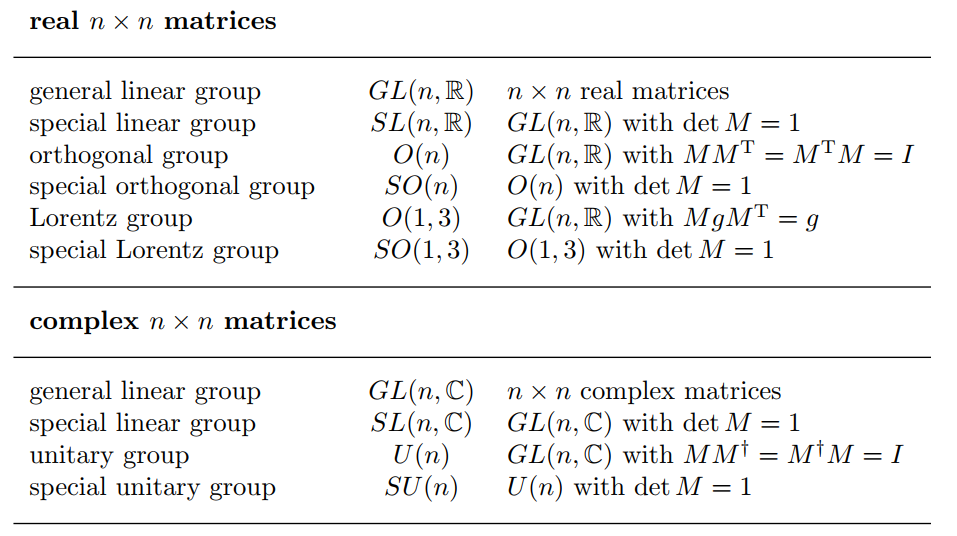
\includegraphics[scale=0.5]{Figures/Lie-Groups.png}
	\caption{Some examples of Lie groups}
\end{figure}
Some of these groups have interesting relations between them
\begin{figure}
	\centering
	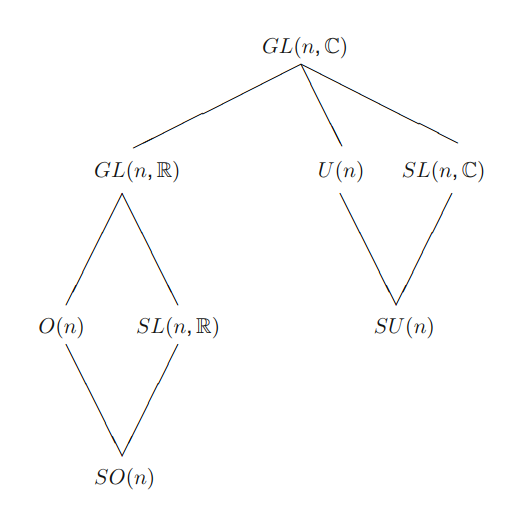
\includegraphics[scale=0.5]{Figures/cat-diag.png}
	\caption{Relationships between interesting Lie groups}
\end{figure}
\subsubsection{Generators}
We can parameterize all group elements in a form
\begin{equation}
    \left g(\alpha_{i}) \right \vert_{\alpha_{i} = 0} = e
\end{equation}
and we can consider a matrix group representation of this as
\begin{equation}
   \left  D_{n}(g(\alpha_{i})) \right \vert_{\alpha_{i} = 0} = \mathbb{I}
\end{equation}
Where we term $D_{n}$ the \textbf{representation} (we will define this clearly in the following sections) and $\mathbb{I}$ as the $n \times n$ identity matrix. Now let's take a $\delta \alpha_{i} << 1$. We can then taylor expand $D_{n}$ as,
\begin{equation}
    D_{n}(g(\delta \alpha_{i})) = \mathbb{I} + \delta \alpha_{i} \left \frac{\partial D_{n}(g(\alpha_{i}))}{\alpha_{i}} \right \vert_{\alpha_{i} = 0} + ...
\end{equation}
The leading order term is so important that we give it a label of the form
\begin{equation}
    X_{i} = -i\left \frac{\partial D_{n}(g(\alpha_{i}))}{\alpha_{i}} \right \vert_{\alpha_{i} = 0}
\end{equation}
Where $X_{i} \in M_{n}$ and the $-i \ $ has been included to ensure hermicity. Thus, we have the form \footnote{We have switched notation here, $D_{n}(g(\delta \alpha_{i})) = D_{n}(\delta \alpha_{i})$ for brevity}
\begin{equation}
    D_{n}(\delta \alpha_{i}) = \mathbb{I} + i \delta \alpha_{i} X_{i} + ...  
\end{equation}
Now if we want to consider finite transformations such as those parameterized by $alpha_{i}$, we can say that it can be constructed out of an infinite number of infinitesimal transformations
\begin{equation}
    \alpha_{i} = \lim_{N \rightarrow \infty} N \delta \alpha_{i}
\end{equation}
Thus we can rewrite in terms of our taylor expansion as\footnote{}
\begin{equation}
    \lim_{N \rightarrow \infty}{(\mathbb{I} + i \delta \alpha_{i}X_{i})}^{N} = \lim_{N \rightarrow \infty}{(\left \mathbb{I} + i \frac{\alpha_{i}}{N}X_{i} \right)}^{N}
\end{equation}
If we expand this out for several values of $N$, we will see that
\begin{equation}
    \lim_{N \rightarrow \infty}{(\left \mathbb{I} + i \frac{\alpha_{i}}{N}X_{i} \right)}^{N} = e^{i \alpha_{i}X_{i}}
\end{equation}
We call the $X_{i}$'s the \textbf{generators} of the group, which are related to the group elements through the exponential map. The number of generators of a group is termed the group's \textbf{dimension}.
\subsubsection{The Matrix exponential}
The matrix exponential is defined as,
\begin{equation}
    exp: M_{n}(\mathbb{C}) \rightarrow GL(n, \mathbb{C})
\end{equation}
for example,
\begin{equation}
    x \rightarrow \sum^{\infty}_{k=0} \frac{x^{k}}{k!}
\end{equation}
this converges for all $x$. Some interesting things about the matrix exponential:
\begin{itemize}
    \item $exp$ is surjective
    \item $e^{A. X.A^{-1}} = A e^{X}A^{-1} \ \forall \ A \in GL(n,\mathbb{C})$
    \item $det(e^{X}) = e^{tr(X)}$
    \item $e^{0} = \mathbb{I}$
    \item ${(e^{X})}^{*} = e^{X^{*}}$
    \item ${(e^{X})}^{T} = e^{X^{T}}$
    \item ${(e^{X})}^{-1} = e^{X^{-1}}$
    \item $e^{(\alpha + \beta)X} = e^{\alpha X}e^{\beta X} \ \forall \ \alpha, \beta \in \mathbb{C}$
    \item If $XY = YX$ then $e^{X + Y} = e^{X}.e^{Y} = e^{Y}.e^{X}$
    \item In general, $e^{X + Y} = \lim_{k \rightarrow \infty} (e^{X/k}.e^{Y/k})$. This is called the Lie product formula
    \item $\frac{d}{d \epsilon} e^{\epsilon X} = X e^{\epsilon X} = e^{\epsilon X} X\ \forall \epsilon \in \mathbb{R}$
    \item $\left \frac{d}{d \epsilon}  \right \vert_{\epsilon = 0 } e^{\epsilon X} = X $
    \item $e^{\epsilon X} = e^{\epsilon Y} \ \forall \ \epsilon \in \mathbb{R} \leftrightarrow X = Y$
\end{itemize}

\subsubsection{Lie Algebra}
A Lie Algebra $\mathfrak{g}$ is a vector space over some field $\mathcal{F}$ together with a binary operation $\left[,\right] := \mathfrak{g} \times \mathfrak{g} \rightarrow \mathfrak{g}$ called the Lie bracket satisfying the following axioms $\forall \ x, y,z \in \mathfrak{g} ; \forall \ a,b \in \mathcal{F}$:
\begin{itemize}
    \item \textbf{Bilinearity}
    \begin{itemize}
        \item $\left[ ax + by, z \right] = a\left[x,z\right] + b	\left[y,z\right]$
			\item $\left[ z, ax + by \right] = a\left[z,x\right] + b	\left[z,y\right]$
    \end{itemize}
    \item \textbf{Alternativity:} $\left[ x, x \right] = 0$	
    \item \textbf{Jacobi Identity:} $\left[ x, \left[ y,z \right] \right] + \left[ z, \left[ x, y \right] \right] + \left[ y, \left[ z,x \right] \right] = 0$
    \item \textbf{Anticommutativity:} $ \left[ x,y \right] = -\left[ y,x \right]$	
\end{itemize}

\subsubsection{Single-Parameter Lie groups}
A one-parameter group or one-parameter subgroup usually means a continuous group homomorphism from the real line $\mathbb{R}$ as an additive group i.e. where the group composition is addition to some other topological group G . If $\phi$ is injective then $\phi(\mathbb{R})$, the image, will be a subgroup of $G$ that is isomorphic to $\mathbb{R}$ as an additive group.
\begin{equation}
    \phi : \mathbb{R} \rightarrow G 
\end{equation}
This is how infinitesimal transformations were defined by Lie: "an infinitesimal transformation is an infinitely small transformation of the one-parameter group that it generates"

\subsubsection{Interesting things about Lie groups}
\begin{itemize}
    \item $G \leq GL(n,\mathbb{R})$ are termed compact if it is closed and bounded w.r.t. $M_{n}(\mathbb{C})$
    \item We term $G$ to be connected if for every $g \in G$ there is continuous path connecting it to the identity
    \item $G$ is termed simply connected if every loop can be shrunk to a single point i.e. no holes
    \item If $X \in \mathfrak{g}$ then $\{e^{\epsilon X} | \epsilon \in \mathbb{R}\}$ is a one parameter subgroup of $G$
    \item In fact every smooth i.e. continuous one-parameter subgroup of $G$ is of this form
    \item If $G$ is connected then every group element can be written down as an exponential map where the generators are elements of the Lie algebra
    \item All homomorphisms and isomorphisms are continuous
\end{itemize}
\subsection{Representation Theory}
A group homomorphism $\pi$ is a representation if it's domain is $GL(V)$ for some vector space $V$ 
\begin{equation}
    \pi: G \rightarrow GL(V)
\end{equation}
For all $g \in G$, two representations $\pi_{1}(g) \rightarrow V_{1}$ and $\pi_{2}(g) \rightarrow V_{2}$ are considered \textbf{equivalent} if there is a matrix $A: V \rightarrow V$ such that
\begin{equation}
    \pi_{1}(g) = A^{-1} \pi_{2}(g) A
\end{equation}
 Here, $A$ is termed a \textbf{similarity transform}. Let's say we have two representations $\pi_{1}: G \rightarrow V_{1}$ and $\pi_{2}: G \rightarrow V_{2}$, we can then define a new representation $\pi$ of the form
\begin{equation}
    (\pi_{1}\oplus\pi_{2})(g) = \pi_{1}(g)\oplus\pi_{2}(g) = \begin{pmatrix}
\pi_{1}(g) & 0 \\
0 & \pi_{2}(g)
\end{pmatrix}
\end{equation}
This matrix form is often called the block-diagonal form. In the above example and are called the sub-representations of $\pi$. An \textbf{irreducible representation} (often called an “irrep”) is a representation with no sub-representations (except for the trivial one and itself).
%\subsection{Important Theorems}
%\subsubsection{Lagrange's Theorem}
%\begin{tcolorbox}
 %   For any finite group G, the order (number of elements) of every subgroup of G is  equal to the number of of left cosets of $H$ in $G$
%\end{tcolorbox}
%\subsubsection{Cayleys's Theorem}
%\begin{tcolorbox}
 %   Every group $G$ is isomorphic to a subgroup of the symmetric group acting on $G$
%\end{tcolorbox}
%\subsubsection{Schur's Lemma}
%\begin{tcolorbox}
    
%\end{tcolorbox}
\section{Variational Calculus}
\subsection{A Lemma}
If,
\begin{equation}
    \int_{a}^{b}A(t)\eta(t)dt =0
\end{equation}
where,
\begin{itemize}
    \item $\eta(a) = \eta(b) = 0$
    \item $A(t)$ and $\eta(t)$ are both twice differentiable in the closed interval $[a,b]$ 
\end{itemize}
then,
\begin{tcolorbox}
$A(t) = 0$ throughout $[a,b]$
\end{tcolorbox}
\subsubsection{Proof by Contradiction}
Suppose that there exists $A(c) \neq 0$ for some $a < c < b$. For definiteness let's also suppose that $A(c) > 0$. Due to the continuity of $A(t)$, an interval $[t_{1},t_{2}]$ about c but within $[a,b]$ exists on which A(t) > 0. However under these conditions we can construct a $\eta(t)$ that leads to the integral being non-zero. For example,
\begin{equation} \label{deltadef}
\eta(t) =  
\begin{cases}
{(t-t_{1})}^{3}{(t_{2}-t)}^{3}, & \text{for } t_{1} < t < t_{2}\\
0, & \text{for } t < t_{1} \text{ and } t > t_{2}
\end{cases}
\end{equation}
this $\eta(t)$ has continuous second derivative throughout $[a,b]$ and meets the stated boudary conditions , however the integral does not vanish contrary to the statement. To prevent this thus, it must be $A(t)$ that must vanish throughout $[a,b]$.

\subsection{Deriving the Euler-Lagrange Equations}
The goal here is to find the extremal of the functional
\begin{equation}
			J(\alpha) = \int_{x_{2}}^{x_{1}}f\{y(\alpha , x),y^{'}(\alpha , x);x \} dx
		\end{equation}
		That is $\forall \ \eta(x)$, we want to find
		\begin{equation}
		\left. \frac{\partial J}{\partial \alpha} \right |_{\alpha = 0}  = 0
		\end{equation}
		Where $\alpha$ is a parameter.We thus start by, parameterizing $y$ as,
		\begin{equation} \label{increment}
		    y(x) = y(0) + \alpha \eta(x)
		\end{equation}
\begin{figure}
	\centering
	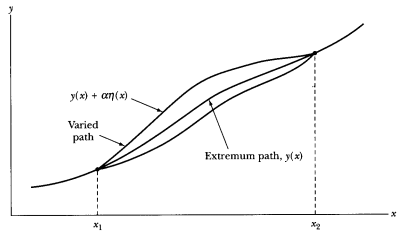
\includegraphics[scale=0.8]{Figures/var.png}
	\caption{We can think of this as trying to find the extremized path from a perturbed one}
\end{figure}
	We can now take the derivative
\begin{equation}
\frac{\partial J}{\partial \alpha} = \frac{\partial}{\partial \alpha}\int_{x_{2}}^{x_{1}}f\{y(\alpha , x),y^{'}(\alpha , x);x \} dx
\end{equation}
\begin{equation} \label{eq-varpar}
    \frac{\partial J}{\partial \alpha} = \int_{x_{2}}^{x_{1}} \left(\frac{\partial f}{\partial y}\frac{\partial y}{\partial \alpha} + \frac{\partial f}{\partial y^{'}}\frac{\partial y^{'}}{\partial \alpha} \right) dx
\end{equation}
From Equation (\ref{increment}) we have
\begin{align}
\frac{\partial y}{\partial \alpha} = \eta(x) \ ; \  & \frac{\partial y^{'}}{\partial \alpha} = \frac{d \eta}{d x}
\end{align}
Plugging this back in to equation (\ref{eq-varpar})
	$$\frac{\partial J}{\partial \alpha} = \int_{x_{2}}^{x_{1}} \left(\frac{\partial f}{\partial y}\eta(x) + \frac{\partial f}{\partial y^{'}}\frac{\partial \eta}{\partial x} \right) dx$$	
	The second term in the integrand can be integrated by parts:
	$$\int_{x_{1}}^{x_{2}} \frac{\partial f}{\partial y^{'}}\frac{d \eta}{dx} dx = \left \frac{\partial f}{\partial y^{'}} \eta(x) \right |^{x_{2}}_{x_{1}} -\int_{x_{1}}^{x_{2}} \frac{d}{dx} \left(\frac{\partial f}{\partial y^{'}}\right)\eta(x) dx $$
	$$\frac{\partial J}{\partial \alpha} = \int_{x_{1}}^{x_{2}} \left(\frac{\partial f}{\partial y} - \frac{d}{dx}\frac{\partial f}{\partial y^{'}} \right) \eta(x) dx$$
	\begin{tcolorbox}
		\begin{equation}
		\frac{\partial f}{\partial y} - \frac{d}{dx}\frac{\partial f}{\partial y^{'}} = 0
		\end{equation}
	\end{tcolorbox}
\subsection{Special Notation}
	We have the equation
\begin{equation}
\frac{\partial J}{\partial \alpha} d\alpha = \int_{x_{1}}^{x_{2}} \left(\frac{\partial f}{\partial y} - \frac{d}{dx}\frac{\partial f}{\partial y^{'}} \right) \frac{\partial y}{\partial \alpha} d \alpha dx = 0
\end{equation}
It can be written as 
\begin{equation}
\delta J = \int_{x_{1}}^{x_{2}} \left(\frac{\partial f}{\partial y} - \frac{d}{dx}\frac{\partial f}{\partial y^{'}} \right) \delta y \ dx = 0
    \end{equation}
where
\begin{equation}
\begin{cases}
\frac{\partial J}{\partial \alpha} d\alpha = \delta J\\
\frac{\partial y}{\partial \alpha} d\alpha = \delta y
\end{cases}
\end{equation}
The condition of extremum then becomes,
\begin{equation}
\delta J = \delta \int_{x_{1}}^{x_{2}} f\{y, y^{'}; x\} dx = 0
\end{equation}
Sometimes we term this the functional derivative i.e. the Frechet derivative
\begin{equation}
    \frac{\delta J}{\delta y} = \frac{\partial f}{\partial y} - \frac{d}{dx}\frac{\partial f}{\partial y^{'}}
\end{equation}

\subsection{The Legendre Transform}
The Legendre transform is way of renaming the dependent variables of a functional. For example, consider the following function $f(x,y)$ whose total derivative is
\begin{equation}
    df = \frac{\partial f}{\partial x}dx + \frac{\partial f}{\partial y}dy 
\end{equation}
Now let's define a new function $g(x,y,u)$, whose total derivative looks like
\begin{equation}
    dg = d(ux) - df = udx + xdu - \frac{\partial f}{\partial x}dx - \frac{\partial f}{\partial y}dy
\end{equation}
However if we define,
\begin{equation}
    u(x,y) = \frac{\partial f}{\partial x}
\end{equation}
Then the term proportional to $dx$ vanishes i.e. we get
\begin{equation}
    dg = xdu - \frac{\partial f}{\partial y}dy
\end{equation}
We can thus consider $g$ as simply a function of  $u$ and $y$ by defining $x := x (u,y)$ that is
\begin{equation}
    g(u,y) = ux(u,y) - f(x(u,y),y)
\end{equation}
This is called the Legendre transform. It takes one function to another by renaming one of it's dependent variable's derivatives. However we haven't lost any information about the original function, as from the identities
\begin{equation}
    \begin{align}
        \left \frac{\partial g}{\partial u} \right |_{y} = x(u,y) \ \ \text{and} \ \ \left \frac{\partial g}{\partial y} \right |_{u} =  -\frac{\partial f}{\partial y}
    \end{align}
\end{equation}
we can get back the original function through the inverse Legendre transform $f = (\partial g/ \partial u)u - g$
\section{Probability Distributions}
\subsection{Discrete Distributions}
Suppose we have a frequency distribution 
\begin{equation}
N = \sum_{j=0}^{\infty} N(j)
\end{equation}
The probability of an event $N_{j}$ is defined as,
\begin{equation}
P(j) = \frac{N(j)}{N}
\end{equation}
In probability theory, the sum of all probabilities is 1,
\begin{equation}
\sum_{j = 0}^{\infty}P(j) = \sum_{j = 0}^{\infty}\frac{N(j)}{N} = 1
\end{equation}
The average/mean/expectation value of a value $j$ is given by the formula:
\begin{equation}
	\expval{j} = \frac{\sum j N(j)}{N} = \sum_{j =0 }^{\infty} j P(j)
\end{equation}
and in general, the average of some function of $j$, is given by,
\begin{equation}
\expval{f(j)} = \sum_{j =0 }^{\infty} f(j) P(j)
\end{equation}
The spread of a variable's value from it's mean is called it's variance, written as
\begin{equation}
\sigma^{2} = \expval{{(\Delta j)}^{2}}
\end{equation}
where,
$$\Delta j = j - \expval{j}$$
It's square root is called the standard deviation,
\begin{equation}
\sigma = \sqrt{\expval{{(\Delta j)}^{2}}} =  \sqrt{\expval{j^{2}} - \expval{j}^{2}}
\end{equation}
Which comes from a theorem on variances that we'll find useful later on:
$$\sigma^{2} = \expval{{(\Delta j)}^{2}} = \sum {(\Delta j)}^{2} P(j) = \sum {(j- \expval{j})}^{2} P(j)$$
$$ = \sum (j^{2} - 2j \expval{j} + \expval{j}^{2}) P(j)$$
$$ = \sum j^{2}P(j) - 2 \expval{j} \sum jP(j) + \expval{j}^{2}\sum P(j)$$
$$ = \expval{j^{2}} - 2 \expval{j}\expval{j} + \expval{j}^{2} = \expval{j^{2}} - \expval{j}^{2}$$
\subsection{Continuous Distributions}
We now move to a continuous probability distribution, we'll create continuous analogs of all the quantities we just introduced. Let's start with probability, the probability of that $x$ lies between $a$ and $b$
\begin{equation}
	P_{ab} = \int_{a}^{b} \rho(x) dx
\end{equation}
where $\rho(x)$ is the called the probability density i.e. the probability of getting $x$, or more concretely,
$$\rho(x)dx = \text{Probability that an individual is chosend at random lies between } x \text{ and } x + dx$$
Now supposing the rules we held for discrete variables hold, the continuous analogs look like this:
\begin{equation}
	1 = \int_{- \infty}^{\infty} \rho(x) dx
\end{equation}
\begin{equation}
	\expval{x} = \int_{- \infty}^{\infty} x \rho(x) dx
\end{equation}
\begin{equation}
	\expval{f(x)} = \int_{- \infty}^{\infty} f(x) \rho(x) dx
\end{equation}
\begin{equation}
	\sigma^{2} := \expval{(\Delta x)^{2}} = \expval{x^{2}} - {\expval{x}}^{2}
\end{equation}
%\section{Expectation Values}
%In this section we'll explore how we express the expectation values of a few opeartors. Let's start with the position opeartor in the position representation (i.e. position basis):
%\begin{equation} \label{posex}
	%\expval{x} = \int_{- \infty}^{\infty} x \abs{\psi(\vec{x}, t)}^{2} dx
%\end{equation}
%We can differentiate \ref{posex} with respect to time to find the expectation value for "velocity":
%$$\frac{d \expval{x}}{dt} = $$
%Throwing away 
%\begin{equation}
%	\expval{v} = \frac{d \expval{x}}{dt} = -\frac{i \hbar}{m} \int \psi^{*} \frac{\partial \psi}{\partial x} dx
%\end{equation}
%Therefore we can write the expectation value of momentum as,
%\begin{equation}
%	\expval{p} = m \frac{d \expval{x}}{dt} =  -i \hbar \int \left(\psi^{*} \frac{\partial \psi}{\partial x} \right) dx
%\end{equation}
%In general, every observable is a function of position and momentum, thus for an observable %$\hat{O}(x,p)$, the expectation value is given by,
%\begin{equation}
%	\expval{\hat{O}(x,p)} = \int \psi^{*} \hat{O}(x,-i \hbar \nabla) \psi dx
%\end{equation}
%For example, the expectation value of kinetic energy is,
%\begin{equation}
%\expval{T} = -\frac{\hbar^{2}}{2m} \int \psi^{*} \frac{\partial^{2} \psi}{\partial x^{2}} dx
%\end{equation}
%Or to sum it up in Dirac notation,
%\begin{equation}
%	\expval{\hat{O}} = \expval{\hat{O}}{\psi}
%\end{equation}

\section{Covariant Derivative}
A connection is a tool that allows us to compare prices or phases at different locations since
it keeps track of how the local coordinate systems are defined and encodes information about
the structure of the space we are moving in.
As already mentioned above, there are two situations where it’s necessary to introduce
connections. One the one hand, we need connections to allow arbitrary local coordinate
systems. Here the connection keeps track of these local coordinate systems and lets us
compare prices or phases defined according to different local conventions. On the other
hand, connections are essential whenever the space we are interested in is curved.
The prototypical example of a curved space is a sphere. To compare vectors at two different
points on a sphere (e.g. to calculate a derivative), we need a procedure to move one vector
to the location of the second one consistently.
The needed procedure is known as parallel transport. To understand it imagine we can
imagine that we are walking on the sphere while holding a stick in your hand. While we are
walking we our best to keep the stick straight. If we do this, we are parallel transporting
the stick.
Mathematically, the infinitesimal parallel transport of a vector Vα(x) is defined as
\begin{equation}
V_{\alpha}(x + dx) = V_{\alpha}(x) - \Gamma^{\alpha}_{\beta \gamma}(x)V^{\beta}(x)dx^{\gamma}
\end{equation}
    where $\Gamma^{i}_{jk}$ denotes the corresponding connection.
An important observation is that if the space we are moving in is curved, it’s possible
the stick does not end up in its starting position if we move along a closed curve.
\begin{figure}[!ht]
	\centering
	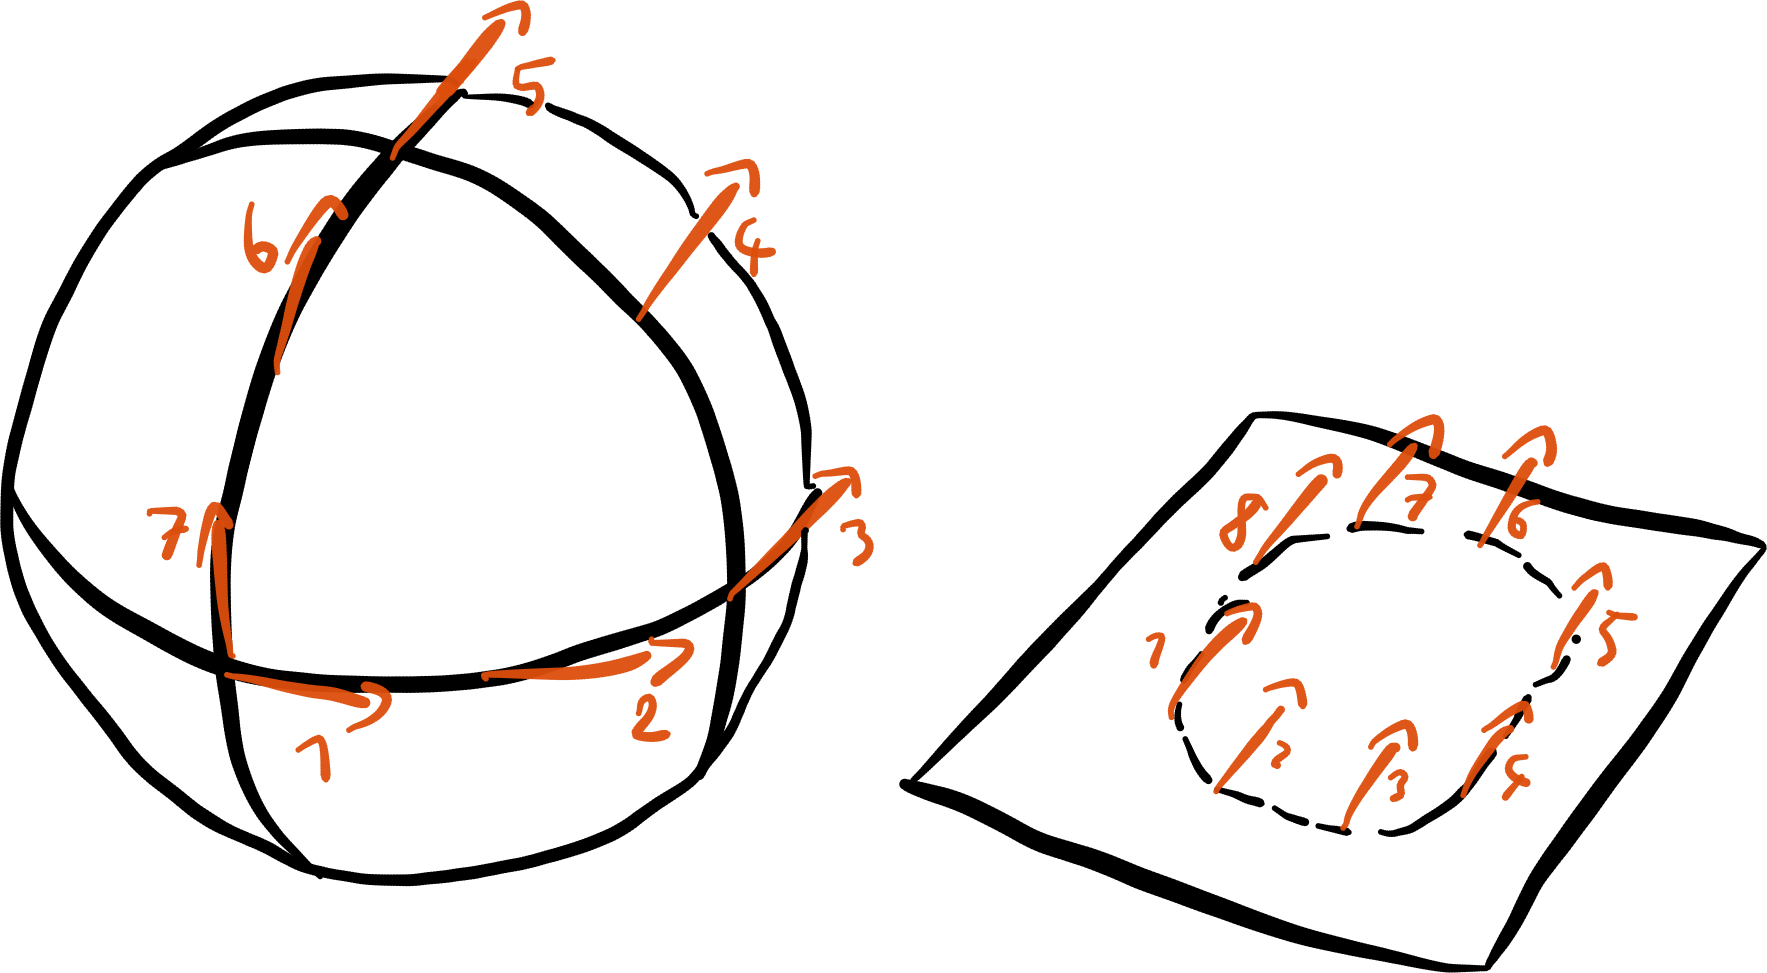
\includegraphics[scale=0.2]{Figures/23-2.png}
	\caption{A pictorial representation of Parallel Transport}
\end{figure}
Hence, the difference between the original vector and the vector which was parallel transported along an infinitesimal closed curve encodes information about the local curvature.
Therefore, to define curvature we imagine that our vector moves from A to B via two different paths.
\begin{figure}[!ht]
	\centering
	
\includegraphics[scale=0.5]{Figures/curvatureloop.png}
	\caption{A pictorial representation of taking two different paths}
\end{figure}
Taken together these two paths yield a closed curve and we can calculate
\begin{equation}
    V_{\alpha}(A \rightarrow C \rightarrow B)  - V_{\alpha}(A \rightarrow D \rightarrow B) = R^{\gamma}_{\alpha \beta \mu}V^{\beta}dx^{\mu}dx^{\nu}
\end{equation}
where $R^{\nu}_{\alpha \beta \mu}$
denotes the corresponding (Riemann) curvature tensor
\begin{equation}
    R^{\nu}_{\alpha \beta \mu} =  \partial_{\alpha}\Gamma^{\mu}_{\beta \nu} - \partial_{\beta}\Gamma^{\mu}_{\alpha \nu} + \Gamma^{\mu}_{\alpha \kappa}\Gamma^{\kapa}_{\beta \nu} - \Gamma^{\mu}_{\beta \kappa}\Gamma^{\kappa}_{\alpha \nu}
\end{equation}
\subsection{The Formalism}
The covariant derivative of a vector field $v^{\mu}$ is defined as,
\begin{equation}
\nabla_{\mu} v^{\alpha} = v^{\alpha}_{ \  ; \mu} = \partial_{\mu} v^{\alpha} + \Gamma^{\alpha}_{\mu \nu} v^{\nu}
\end{equation}
 It is worth noting that the connection i.e. theChristoffel symbol is not a tensor because it contains all the information about the curvature of the coordinate system and can therefore be transformed entirely to zero if the coordinates are straightened. Nevertheless we treat it as any ordinary tensor in terms of the index notation. It can be defined in terms for derivatives as:
\begin{equation}
\Gamma^{k}_{ij}\vec{e}_{k} = \frac{\partial \vec{e}_{i}}{\partial x^{j}}
\end{equation}
Where, the index $i$ specifies the basis vector for which the derivative is being
taken, the index $j$ denotes the coordinate being varied to induce this change
in the $i$th basis vector, and the index $k$ identifies the direction in which this
component of the derivative points. We define the Christoffel symbol in terms of the metric $g_{\mu \nu}$ and it's inverse $g^{\alpha \beta}$ as\footnote{The connection coefficients defined here are of the Levi-Civita Connection. It a unique connection (covariant derivative) that is Torsion-Free and has Metric Compatibility},
\begin{equation}
\Gamma^{\alpha}_{\ \mu \nu} = \frac{1}{2} g^{\alpha \beta} \left(\frac{\partial g_{\beta \nu}}{\partial x^{\mu}} + \frac{\partial g_{\beta \mu}}{\partial x^{\nu}} - \frac{\partial g_{\mu \nu}}{\partial x^{\beta}}\right) = \frac{1}{2}g^{\alpha \beta} \left(g_{\beta \nu, \mu} + g_{\beta \mu, \nu} - g_{\mu \nu, \beta}\right)
\end{equation}
We can then define the covariant derivative of a covector as,
\begin{equation}
\nabla_{\mu} w_{\alpha} = w^{\alpha}_{ \  ; \mu} = \partial_{\mu} w_{\alpha} + \Gamma^{\alpha}_{\mu \nu} w_{\nu}
\end{equation}
The covariant derivative of a tensor $t^{\alpha\beta}$ is then,
\begin{equation}
\nabla_{\mu}t^{\alpha \beta} = \partial_{\mu} t^{\alpha \beta} + \Gamma^{\alpha}_{\mu \sigma}t^{\sigma \beta} + \Gamma^{\beta}_{\mu \sigma}t^{\alpha \sigma }
\end{equation}
and of a tensor $t^{\alpha}_{\beta}$,
\begin{equation}
\nabla_{\mu}t^{\alpha}_{\beta} = \partial_{\mu} t^{\alpha}_{\beta} + \Gamma^{\alpha}_{\mu \sigma}t^{\sigma}_{\beta} + \Gamma^{\beta}_{\mu \sigma}t^{\alpha}_{\sigma}
\end{equation}

\pagestyle{plain} 

% References
\newpage
%\printbibliography
%\addcontentsline{toc}{chapter}{Bibliography}
%\ifUseGermanVersion
%	\bibliographystyle{fhstp-apalike}
%\else
%    \bibliographystyle{apa-good}
%\fi

%\bibliography{Bibliography.bib}

% Figures
\newpage
\listoffigures
\addcontentsline{toc}{chapter}{List of Figures}
% Tables
\newpage
\listoftables
\addcontentsline{toc}{chapter}{List of Tables}
% Listings
\newpage
\lstlistoflistings
\addcontentsline{toc}{chapter}{List of Listings}
\newpage

% ============================================



%\printbibliography
\begin{thebibliography}{9}
    \bibitem {} Goldstein, H., Safko, J., &amp; Poole, C. P. (2014). Classical mechanics. Harlow: Pearson.
    
    \bibitem {} David Tong, Notes on Classical Mechanics
    	
	\bibitem {p} Neuenschwander, D. E. (2017). Emmy Noether's wonderful theorem. Baltimore: Johns Hopkins Univ. Press.
	
	\bibitem{p} Griffiths, D. J. (2018). Introduction to electrodynamics. Cambridge, United Kingdom: Cambridge University Press.
	
	\bibitem {p} Lancaster, T., \& Blundell, S. (2018). Quantum field theory for the gifted amateur. Oxford: Oxford University Press.
	
	\bibitem{p1} Griffiths, D. J. (2005). Introduction to quantum mechanics. Upper Saddle River, NJ: Pearson/Prentice Hall 
	
	\bibitem{p2} Shankar, R (1994). Principles of quantum mechanics. New York: Springer
	
	\bibitem {p12} Larkoski, A. J. (2019). Elementary particle physics: An intuitive introduction. Cambridge University Press 
	\bibitem {p13} Peskin, M. (2018). Concepts of Elementary Particle Physics. Oxford Higher Education 
	
	\bibitem {} Halmos, P. R. (1987). Naive set theory. Berlin u.a.: Springer.
	
	\bibitem {} Stone, M., &amp; Goldbart, P. M. (2010). Mathematics for physics: A guided tour for graduate students. Cambridge: Cambridge University Press.
	
	 \bibitem {p14} Arfken, G., Weber, H. J., \& Harris, F. E. (2013). Mathematical methods for physicists. Amsterdam: Elsevier Academic Press.
	
	\bibitem {p15} Riley, K. F., \& Hobson, M. P. (2008). Mathematical methods for physics and engineering a comprehensive guide. Cambridge: Cambridge University Press.
	
	\bibitem {p16} Artin, M (2018). Algebra.NY, NY: Pearson
	
	\bibitem {p17} Fleisch, D. A. (2018). A student's guide to vectors and tensors. Cambridge: Cambridge University Press
	
	\bibitem {p18} Jeevanjee, N. (2015). An introduction to tensors and group theory for physicists: Nadir Jeevanjee. Cham: Birkhauser.
	
	\bibitem {p19} Das, A. J. (2007). Tensors: The Mathematics of Relativity Theory and Continuum Mechanics. New York: Springer Science Business Media, LLC
	
	 \bibitem {p20} Kees Dullemond \& Kasper Peeters (1991), Introduction to Tensor Calculus 
		
	\bibitem {p21} Nakahara, M. (2017). Geometry, Topology and Physics. Boca Raton, FL: CRC Press.
	
	\bibitem {p22} Neuenschwander, D. E. (2015). Tensor Calculus for Physics: A Concise Guide. Baltimore, MD: JOHNS HOPKINS University Press.
	
	 \bibitem {p23} Oppenheim, A. V., Willsky, A. S., \& Nawab, S. H. (2015). Signals \& systems. Second edition.: Pearson.
    
    \bibitem {p6} Schwichtenberg, J. (2018). Physics from Symmetry. Cham: Springer International Publishing.
    
    \bibitem{} Robinson Matthew. (2011). Symmetry and the standard model: Mathematics and particle physics. New York: Springer.
     
    \bibitem {p33} Needham, T. (2012). Visual complex analysis. Oxford: Clarendon Press.
     
    \bibitem {p} Aivazis, M., \& Tung, W. (2006). Group theory in physics. Singapore: World Scientific.
	
    \bibitem{} Axler, S. (2017). Linear algebra done right. Springer.
    
    \bibitem{} Schwichtenberg, J (2019). Demystifying Gauge Symmetry. History and Philosophy of Physics, arXiv
    
    \bibitem{} Max Planck (1968). Scientific Autobiography and Other Papers. Philosophical Library

    \bibitem{} F. Bloch (1976). Heisenberg and the early days of quantum mechanics. Physics Today, December
    
    
    \bibitem {} Ron Y. Donagi (1997). Seiberg-Witten integrable systems. arXiv:alg-geom/9705010
    
    \bibitem {} Christopher A. Martin (2003).  On continuous symmetries and the foundations of modern physics, Symmetries in Physics, Philosophical Reflections. Cambridge University Press
\end{thebibliography}
% ============================================

\end{document}























